\documentclass[11pt]{article}
\usepackage[T1]{fontenc}
\usepackage[utf8]{inputenc}
\usepackage{lmodern}
\usepackage[letterpaper,margin=0.92in]{geometry}
\usepackage{amsmath,amssymb,mathtools}
\usepackage{adjustbox}
\usepackage{needspace}
\usepackage{microtype}
\usepackage{enumitem}
\usepackage[numbers,sort&compress]{natbib}
\usepackage{tikz}
\usetikzlibrary{arrows.meta,positioning,calc,fit,shapes.geometric,decorations.pathreplacing,angles,quotes}
\usepackage[hidelinks,unicode]{hyperref}
\usepackage{bookmark}

\hypersetup{
  pdftitle={Observer-Rooted Asymmetry},
  pdfauthor={Ray-Scott Miller},
  pdfsubject={A Closure-First Derivation of Charged-Lepton Mass Ratios with Independent Koide Validation}
}
\setcounter{secnumdepth}{2}
\setcounter{tocdepth}{2}
\setlength{\parindent}{1.2em}
\setlength{\parskip}{0.24em}
\setlist{nosep,leftmargin=2em}
\emergencystretch=3em
\allowdisplaybreaks[2]

\begin{document}
\begin{center}
{\LARGE\bfseries Observer-Rooted Asymmetry\par}
\vspace{0.7em}
{\large\itshape A Closure-First Derivation of Charged-Lepton Mass Ratios with Independent Koide Validation\par}
\vspace{0.7em}
{\normalsize\bfseries Ray-Scott Miller\par}
\vspace{0.2em}
{\small Independent Researcher\par}
{\small Prosper, Texas, USA\par}
{\small Corresponding author: \href{mailto:Rayscottmiller@gmail.com}{Rayscottmiller@gmail.com}\par}
\end{center}
\vspace{0.7em}

\begin{abstract}
This paper develops a relational foundation from one physical axiom: existence is relational distinguishability. The resulting strictly positive count-and-transfer arithmetic admits no internal object for absence and requires every operation to preserve relational accountability. Persistence and conserving closure then constrain a presentation by the face-centered-cubic lattice and its rhombic-dodecahedral Voronoi cell. Geometry is not primitive background structure in the construction; it is a downstream exact presentation of completed relational records.

A single designated cell supplies the observer/reference role. The observer does not add consciousness, create orientation, or generate the registered structure. It reads distinctions already carried by the relational record. The rooted two-active/one-idle projector on the three-state carrier has normalized valuation \(2/3\). Its completed action fixes the phase from which six \(D_3\)-related presentations descend to one intrinsic unordered three-amplitude spectrum. The same rational value also occurs in a separately derived four-cell flow count, but that numerical equality does not identify the two objects or their derivations.

The counting adjoint and complete retained incidence book force a quadratic-support law with the single coefficient \(m=1/(2\pi)\). Exact bounds place the intrinsic middle-to-minimum ratio strictly between \(206\) and \(207\). A recoverable one-event/two-preserved-face record then supports two \(206\)-element sets with a common three-root carrier; their free pushout has \(409\) classes. The resulting regular-screen factor acts once on the already formed middle quadratic support.

These steps determine two exact charged-lepton mass ratios before any muon or tau measurement is admitted. One recorded electron mass-energy equivalent supplies the sole conventional scale, producing a complete relative three-entry report. The result is not an absolute prediction of the electron mass, and the middle construction is not presented as a blind held-out prediction because it was developed after exposure to muon data.

Only after the mass-ratio derivation closes is the scale-free Koide functional evaluated. The derived three-entry shape lies approximately \(1.35\) parts per million from the conventional \(2/3\) benchmark. Koide is therefore used here as an independent downstream consistency check, not as an input, fitting condition, or claimed exact identity.

\textbf{Keywords:} relational foundations; discrete geometry; observer asymmetry; charged leptons; mass ratios; Koide relation


\end{abstract}

\section*{Introduction}
\addcontentsline{toc}{section}{Introduction}
The three charged leptons have identical electric charge and spin but sharply different masses. Their mass ratios are accurately reported, yet the origin of the hierarchy is not fixed by those reports themselves. Contemporary particle data organize the electron, muon, and tau as a three-member charged-lepton family \cite{PDG2024}, while precision constants provide conventional comparison standards for their masses and ratios \cite{CODATA2022}. The question addressed here is whether a definite three-rank mass structure can be obtained from a more primitive relational construction without using the measured muon or tau mass as an algebraic input.

The strategy is closure-first. The paper begins with relational distinguishability and a positive count-and-transfer discipline. Persistence, closure, and their bookkeeping consequences are developed before geometric, observer, or empirical language is admitted. A face-centered-cubic presentation with rhombic-dodecahedral cells is then obtained as a downstream relational realization. The matrices used in this development are organizational displays: independently established quantities are placed into typed rows and columns after derivation. Their rectangular arrangement does not generate a scientific relation, and no matrix algebra is used to obtain the charged-lepton result.

Within the resulting geometry, one completed cell is designated as the observer/reference role. \textbf{Observer-rooted asymmetry is the dependence of a lawful report on the observer's rooted ancestry and betweenness position, while the underlying unordered intrinsic spectrum remains presentation invariant.} The observer therefore does not change an intrinsic mass or select a preferred spectral value. Its rooted occurrence fixes the lawful presentation data, and its unique interior ancestry position determines which already formed rank receives the later finite-screen rendering.

The principal mathematical contributions are a single connected derivational sequence. A rooted two-active/one-idle occurrence fixes both a normalized radius and an action aperture. The action supplies the phase of six presentation-equivalent Hermitian operators and hence one intrinsic unordered three-amplitude spectrum. A construction-derived adjoint forces quadratic support with coefficient \(m=1/(2\pi)\). Exact rational bounds then place the middle-to-minimum intrinsic ratio strictly between \(206\) and \(207\). A recoverable one-event/two-preserved-face record supports two \(206\)-element sets sharing one three-root carrier; their free pushout has \(409\) elements. The corresponding regular-screen factor acts only on the rank selected by observer-rooted betweenness. These steps determine the two dimensionless charged-lepton mass ratios. Figure \(\ref{fig:derivation-architecture}\) records this dependency order without adding an inference.

The distinction between derivation and calibration is strict. The spectrum, rank ordering, quadratic-support law, \(206\), \(409\), finite-screen factor, and both dimensionless ratios are derived before any dimensional standard is introduced. The electron supplies the sole conventional reporting scale. Neither a measured muon value nor a measured tau value appears as an algebraic operand. The resulting muon and tau mass-energy equivalents are therefore downstream outputs relative to the electron standard, not independent absolute-mass derivations.

The development history also matters for claim strength. The \(409\) construction was developed after exposure to the muon result. The paper does not present the middle output as a blind held-out prediction, even though the measured muon value is absent from the algebra and no continuous numerical parameter is fitted. A post-derivation comparison with the CODATA recommended adjusted muon-to-electron ratio is reported transparently on that basis.

Koide's charged-lepton relation \cite{KOIDE1983} is likewise not a construction input. It is evaluated only after the mass-ratio report has closed. The word \emph{independent} in the subtitle therefore denotes logical independence from the construction inputs: Koide's relation is not used to choose the phase, radius, rank assignment, integer counts, finite-screen factor, or reporting scale. It does not assert algebraic independence from the derived radius and quadratic-support law.

The paper is organized as follows. Sections 1 and 2 establish relational admission and positive transfer arithmetic. Sections 3--7 develop closure, bookkeeping, geometry, and registration while keeping presentation distinct from authority. Sections 8--11 establish the observer, readout, and one-event/two-face recovery record. Section 12 derives the intrinsic three-rank spectrum and quadratic-support law. Section 13 proves the exact \(206\) interval, constructs \(409\), and establishes observer-rooted middle placement. Section 14 forms the charged-lepton ratios and attaches the electron reporting standard before making the disclosed post-exposure muon comparison. Section 15 evaluates the exact intrinsic and finite-screened Koide quotients as downstream consistency checks.


% ALT TEXT: A forward-only roadmap runs from relational existence through closure, derived FCC/RD geometry, rooted radius and phase, the intrinsic spectrum, quadratic support, 206, 409, the electron reporting standard, charged-lepton mass ratios, and finally the downstream Koide check. Construction nodes, the reporting-standard node, and the validation node have distinct styles.
\begin{figure}[t]
\centering
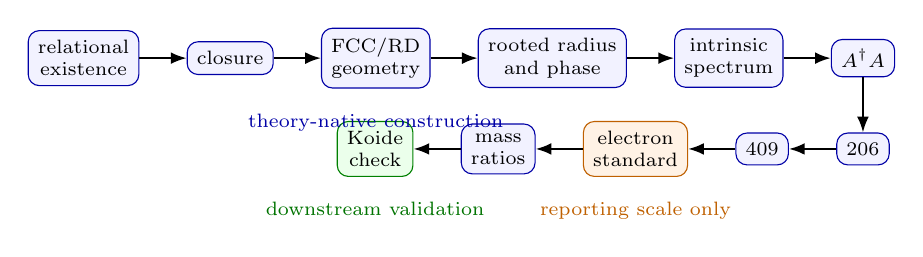
\begin{tikzpicture}[
  node distance=5.5mm and 6mm,
  native/.style={draw=blue!65!black, fill=blue!5, rounded corners,
    align=center, inner sep=3.5pt, font=\scriptsize},
  standard/.style={draw=orange!75!black, fill=orange!10, rounded corners,
    align=center, inner sep=3.5pt, font=\scriptsize},
  validation/.style={draw=green!50!black, fill=green!8, rounded corners,
    align=center, inner sep=3.5pt, font=\scriptsize},
  arrow/.style={-{Latex[length=2mm]}, thick}
]
\node[native] (existence) {relational\\existence};
\node[native, right=of existence] (closure) {closure};
\node[native, right=of closure] (geometry) {FCC/RD\\geometry};
\node[native, right=of geometry] (radius) {rooted radius\\and phase};
\node[native, right=of radius] (spectrum) {intrinsic\\spectrum};
\node[native, right=of spectrum] (support) {\(A^\dagger A\)};
\node[native, below=7mm of support] (n206) {\(206\)};
\node[native, left=of n206] (n409) {\(409\)};
\node[standard, left=of n409] (electron) {electron\\standard};
\node[native, left=of electron] (ratios) {mass\\ratios};
\node[validation, left=of ratios] (koide) {Koide\\check};
\draw[arrow] (existence) -- (closure);
\draw[arrow] (closure) -- (geometry);
\draw[arrow] (geometry) -- (radius);
\draw[arrow] (radius) -- (spectrum);
\draw[arrow] (spectrum) -- (support);
\draw[arrow] (support) -- (n206);
\draw[arrow] (n206) -- (n409);
\draw[arrow] (n409) -- (electron);
\draw[arrow] (electron) -- (ratios);
\draw[arrow] (ratios) -- (koide);
\node[font=\scriptsize, below=2mm of geometry, text=blue!65!black]
  {theory-native construction};
\node[font=\scriptsize, below=2mm of electron, text=orange!75!black]
  {reporting scale only};
\node[font=\scriptsize, below=2mm of koide, text=green!45!black]
  {downstream validation};
\end{tikzpicture}
\caption{Derivation architecture.  Blue nodes belong to the theory-native
construction, the orange electron node supplies only the reporting scale, and
the green Koide node is downstream validation.  Every arrow points forward;
no empirical standard or validation result feeds back into the construction.}
\label{fig:derivation-architecture}
\end{figure}

\Needspace{7\baselineskip}
\section{Relational Existence: The Foundational Axiom}
\label{sec:01}
Section 1 begins with the simplest possible starting point:

\begin{quote}
\textbf{There is something rather than nothing.}
\end{quote}
At first glance, this appears almost trivial. The central claim of this paper is that this starting point, once stated in its precise relational form, is strong enough to force a large amount of structure. The paper does not begin by assuming a manifold, a metric, a field, a background clock, or an external observer. It begins by asking what must be true before any of those notions can even be discussed.

The purpose of this section is therefore not to introduce physics directly. It establishes the admission rules that any later physics must satisfy. At the most fundamental level, no later observer is allowed to stand outside the relational system with access to arbitrary abstractions. Any later observer must be treated as part of the relational system it reads. Before continuous measurement, coordinate systems, or calibrated units, the primitive operation available at this layer is distinguishability: to separate one admitted content from what it is not, and to count what has been admitted.

\Needspace{5\baselineskip}
\subsection{The Existence Axiom}
The most basic question is simply:

\begin{quote}
\textbf{Is there something, or is there nothing?}
\end{quote}
If there is truly nothing, then there is nothing to describe, no distinction to make, no theory to construct, and no standpoint from which even the denial could be stated. A physical theory can only concern what exists. This leaves a boundary and an entry:

\begin{itemize}
\item \(0\): nothing exists. This is the boundary case. It admits no description and no theory.
\item \(1\): something exists. At least one distinction can be made.
\end{itemize}
Only the second case can carry a theory. But "something exists" already contains a distinction. To say that something exists is to distinguish it: from nothing, and from what it is not. Existence never arrives as a bare object to which distinguishability is later added. It arrives, if it arrives at all, as distinguishability within a relation. The paper therefore takes as its single physical axiom:

\begin{quote}
\textbf{Axiom 1 (relational existence).} Existence is relational distinguishability.
\end{quote}
The first number of the theory is not a second assumption. One primitive act of distinguishability is one binary cut, and only the admitted side of that cut enters the theory. The first admitted content is therefore exactly one distinction, with count

\begin{equation*}
\begin{adjustbox}{max width=\linewidth,center}
$\displaystyle
I = 1 .
$
\end{adjustbox}
\end{equation*}
Here \(I\) denotes the first existence count. This is not yet a statement about particles, space, time, fields, or geometry. It is the minimal assertion that there is something rather than nothing, made precise as distinguishability. That precision is what gives the rest of the theory something to build from.

\Needspace{5\baselineskip}
\subsection{Consequences of the Existence Axiom}
Once the first count \(I=1\) is admitted, the unit itself has a special status. It is not composed of smaller units of the same kind inside the theory, because then those smaller units would be the true primitives. The first unit of existence is therefore indivisible within this admission layer, and \(1\) is the natural primitive count.

Larger internal quantities arise only by counting further admitted units:

\begin{equation*}
\begin{adjustbox}{max width=\linewidth,center}
$\displaystyle
1,\ 2,\ 3,\ \dots
$
\end{adjustbox}
\end{equation*}
This is an ontological statement before it is a statement about numerical technique. The theory begins with admitted positive counts. Fractions, decimals, limits, and other numerical representations are not introduced here as new primitive existents. They may enter later as comparison reports, scale choices, limiting descriptions, or licensed mathematical language, but they are not the starting ontology of the theory.

This restriction concerns primitive admission, not the symbols available after a quantity has been derived. For an already established quantity, number class alone neither grants nor denies admissibility. An exact rational, irrational, algebraic, or transcendental expression remains a downstream representation of its typed object; it does not add another primitive relation-token. Its scientific warrant comes from the owning derivation, domain, and guards, not from the notation by itself.

Zero has a different status. It does not represent an existing object or quantity. It marks absence. Since the theory begins from the admitted case that there is something rather than nothing, zero is never treated as a primitive element of the ontology. It may be useful as an external boundary label or inside a controlled formal statement, but it is not an admitted object, primitive internal value, or held quantity. The bookkeeping keeps this distinction sharp: if no transfer occurred, the theory records that no transfer occurred, not a transfer of size zero; if a register is absent, it records absence, not a hidden holding of zero. A detector that did not fire and a detector that fired and read zero are different physical situations. Internally, presence is positive by type:

\begin{equation*}
\begin{adjustbox}{max width=\linewidth,center}
$\displaystyle
q \in \mathcal{D}_+ .
$
\end{adjustbox}
\end{equation*}
The same discipline applies to negative quantities. A negative sign is not interpreted as the existence of negative objects. It is a relational or oriented bookkeeping descriptor applied to positive content. If Alice has three apples and Bob receives two of them, nothing negative has been created. The relationship has changed: Alice now has one apple, Bob has two, and the transfer has an orientation. The internal formalism represents such orientation without turning negative objects into ontology.

A natural worry is that forbidding primitive negative quantities cripples the algebra physicists rely on, especially cancellation. It does not. Within a fixed kind of quantity, cancellation is not assumed as an additional physical axiom; it is a theorem:

\begin{equation*}
\begin{adjustbox}{max width=\linewidth,center}
$\displaystyle
a+q=b+q \Longrightarrow a=b .
$
\end{adjustbox}
\end{equation*}
The reason is simple. In the positive domain, adding something is never adding nothing. The order says that one quantity exceeds another when it differs by a strictly positive gap, and like quantities are comparable. If \(a+q=b+q\) but \(a\neq b\), one side must exceed the other by a positive gap. Adding the same \(q\) to both would then make a sum strictly exceed itself, which positivity forbids. The gap, when it exists, is unique. The theory therefore has the restricted subtraction it needs: not by introducing inverse elements or signed completion, but by reading subtraction as the unique positive gap exhibited by the order.

The result is a root discipline: the theory owns positive admitted content. Zero is absence, and negative signs are relational descriptors rather than primitive objects.

\Needspace{5\baselineskip}
\subsection{No External Background}
An important consequence of the existence axiom is that there can be no independently existing background against which reality is measured.

% LAYOUT_ONLY_GUARD:FIRST_COUNT_BACKGROUND
\Needspace{8\baselineskip}
If the primitive content of the theory is a single admitted distinction, the first count

\begin{equation*}
\begin{adjustbox}{max width=\linewidth,center}
$\displaystyle
I = 1 ,
$
\end{adjustbox}
\end{equation*}
then that admitted distinction is all that is available at the fundamental level. Nothing external to it can be assumed. An independently existing coordinate grid, background space, or absolute reference frame cannot be introduced as an additional primitive, because doing so would add structure beyond the original axiom.

Consequently, geometry, measurement, distance, orientation, and reference may enter only as later relational constructions that preserve the primitive admission discipline. Nothing may be borrowed from an external framework.

This is stronger than saying that the theory merely chooses not to assume a background coordinate system. Within this framework, such a background cannot be introduced as a theory-native primitive: any coordinate system or measurement convention must be introduced as an admitted relational construction from the primitive admission of \(I=1\).

In other words, if one distinction is all that fundamentally exists, then later mathematical and physical structures must earn their place through that relational foundation. Nothing can be assumed to exist outside it.

\Needspace{5\baselineskip}
\subsection{Measurement as Relational Comparison}
The same relational discipline applies to measurement.

The numerical values that appear in physics - integers, decimals, coefficients, and constants - are often treated as intrinsic properties of physical systems. In this framework they are read differently. A measured value is a relational readout: a comparison between admitted content and an admitted reference standard.

A unit of measurement is therefore not fundamental. It is a convention that selects a comparison standard. A gram, for example, is not a primitive physical object. When a report says that an object has a mass of ten grams, the report is comparing that object to a chosen standard about ten times over. The reference standard serves as the counting unit within that measurement convention.

The theory states this before any observer or apparatus has been constructed inside it. Which relation functions as the observer, readout locus, registration relation, or clockhood standard is built later, especially in Section 8. Section 1 fixes only the prior admissibility condition any later measurement report must satisfy. Let \(\operatorname{Adm}(x)\) mean that \(x\) is admitted as a distinguishable relation, let \(L\) denote a future readout context, let \(s\) denote the comparison standard, and let \(\operatorname{Cmp}_L(x,s)\) denote the licensed comparison relation. Then a measurement report is well defined exactly when its full comparison structure is present:

\begin{equation*}
\begin{adjustbox}{max width=\linewidth,center}
$\displaystyle
\operatorname{Meas}_L(x;s)\downarrow
\Longleftrightarrow
\operatorname{Adm}(x)
\wedge
\operatorname{Std}_L(s)
\wedge
\operatorname{Cmp}_L(x,s).
$
\end{adjustbox}
\end{equation*}
The standard itself must be admitted:

\begin{equation*}
\begin{adjustbox}{max width=\linewidth,center}
$\displaystyle
\operatorname{Std}_L(s) \Longrightarrow \operatorname{Adm}(s).
$
\end{adjustbox}
\end{equation*}
The excluded alternative is the primitive scalar: a measured value of a thing alone, belonging to no comparison.

\begin{equation*}
\begin{adjustbox}{max width=\linewidth,center}
$\displaystyle
\neg \exists q\,
\left(
\operatorname{PrimitiveScalar}(q)
\wedge
q=\operatorname{Meas}_L(x)
\right).
$
\end{adjustbox}
\end{equation*}
% LAYOUT_ONLY_GUARD:UNIT_DEFINITION
\Needspace{8\baselineskip}
A reading taken against no standard is not an imprecise measurement. It is not a measurement at all. A unit is a selected admitted standard,

\begin{equation*}
\begin{adjustbox}{max width=\linewidth,center}
$\displaystyle
\operatorname{Unit}_L(s) :=
\operatorname{Adm}(s)\wedge \operatorname{Std}_L(s),
$
\end{adjustbox}
\end{equation*}
and a reported value has the form

\begin{equation*}
\begin{adjustbox}{max width=\linewidth,center}
$\displaystyle
\operatorname{Report}_L(x;s)=q_s(x) ,
$
\end{adjustbox}
\end{equation*}
defined only when the object, the unit role, and the comparison relation are all present. This separates fundamental existence from measurement conventions. SI units and other human-scale units can communicate observer-scale reports consistently, but they are not fundamental ingredients of the internal theory. They enter only when the theory is translated into observer-scale quantities for comparison, especially in Sections 8 and 14.

\Needspace{5\baselineskip}
\subsection{Why Geometry}
The relational foundation also motivates the mathematical language used later.

Geometry is natural for a relational theory because geometry is about relations: position, orientation, adjacency, separation, order, and comparison. A point alone says almost nothing. It becomes meaningful only inside a structure that gives it relations. Geometry is therefore licensed here as relational mathematics, not as primitive ontology. The paper may use geometric language when that language preserves the admitted relations it claims to represent.

This distinction matters. The license does not say that a geometric object is primitive reality, and it does not introduce a lattice, continuum, coordinate system, metric, or physical realization at Section 1. It says that when later sections use geometry, they must use it as a faithful relational presentation rather than as an external background imposed on the theory.

The bookkeeping analogy is useful but only as an analogy. In double-entry accounting, no entry is meaningful in isolation; each posting exists through its relationship to the rest of the books. The present theory has a similar discipline, but it does not import signed ledger arithmetic. Its internal form is strictly positive transfer read through oriented sides. Relationship is the constraint; isolated quantity is not the primitive.

Maintaining that discipline keeps later mathematics from smoothing away the discrete counting basis from which the theory begins. A formalism can be internally consistent and still fail to represent the physical structure if it imports a background or treats a reporting convention as primitive content.

\Needspace{5\baselineskip}
\subsection{The Overall Program}
The program of this paper is to begin with the minimal existence axiom and develop, through forced relational constructions, the geometry later read by an embedded observer.

Many mathematical objects used in physics - negative values, fractional values, irrational quantities, imaginary quantities, and other abstractions - are not taken here as primitive features of the ontology. They may enter as mathematical language, relational structure, comparison structure, or observer-scale report, but not as starting assumptions. The starting operation is simpler:

\textbf{The starting operation is to count admitted distinctions.}

Every later scientific object must be constructed from or typed against that relational ground. This requirement does not force every exact downstream representation to be an integer.

As the theory develops, ledger closure becomes a persistence condition, and later forced relational geometry selects a definite FCC/RD realization. Observer readout and bridge comparison enter only after their own obligations have been stated and checked. The closing sections compare the count structure those later constructions force against measured physics under explicit comparison criteria.

Because the paper ends at such comparisons, its construction discipline is part of its physical content. Nothing in what follows is derived from structure introduced later than it. A numerical success found downstream is never cited as the reason an earlier rule holds. Junction, readout, bridge, and prediction constructions enter only when their obligations have been stated and checked. Naming an obligation is not discharging it.

This foundation can also lose, and it says how. Exhibit an admitted existent with no relational distinguishability - a primitive bare existence apart from any distinction - and Axiom 1 falls. Exhibit a physical measurement that is genuinely a primitive scalar, reducible to no comparison against an admitted standard, and the measurement rule falls. Exhibit a quantity domain with the stated positive-domain properties in which cancellation fails on a concrete triple, and the cancellation theorem fails. Each failure mode is specific and checkable.

The purpose of Section 1 is simply to establish this foundational ontology and mathematical discipline. Everything derived in the remainder of the paper stands on it.


\Needspace{7\baselineskip}
\section{Relational Arithmetic: Formalizing the Relational Ledger}
\label{sec:02}
Section 2 takes the conceptual ideas introduced in Section 1 and begins expressing them in formal mathematics. It gives the arithmetic the theory is allowed to use once a distinction has been admitted, but before metric geometry, observer-local measurement, calibration, or empirical comparison are available. This arithmetic is not a copy of ordinary signed algebra. It is a bookkeeping language for relations.

The central idea is that, at any formal state, the theory maintains a ledger recording which relationships currently contain admitted content. This ledger represents the current admitted state of existence within the relational system.

\Needspace{5\baselineskip}
\subsection{The Holding State}
To formalize the ledger, let \(R\) be a finite set of relationship registers. A holdings state is a partial map

\begin{equation*}
\begin{adjustbox}{max width=\linewidth,center}
$\displaystyle
h:\operatorname{supp}(h)\to \mathcal{D}_+,\qquad
\operatorname{supp}(h)\subseteq R ,
$
\end{adjustbox}
\end{equation*}
assigning to each held register a strictly positive quantity. The quantity domain \(\mathcal{D}_+\) is the positive domain of Section 1: it has no internal zero object, no subtraction operation, and no additive inverses, and adding something is never adding nothing:

\begin{equation*}
\begin{adjustbox}{max width=\linewidth,center}
$\displaystyle
\forall x,y\in\mathcal{D}_+,\qquad x+y\neq x .
$
\end{adjustbox}
\end{equation*}
% LAYOUT_ONLY_GUARD:ABSENCE_DEFINITION
\Needspace{8\baselineskip}
The important point is that this is more than simply saying that zero represents absence. The structure of the ledger itself distinguishes between a relationship that holds content and a relationship that is not part of the holding state at all. An empty register does not contain the value zero. It is absent from the current holding state altogether:

\begin{equation*}
\begin{adjustbox}{max width=\linewidth,center}
$\displaystyle
\operatorname{absent}_h(r)\Longleftrightarrow r\notin\operatorname{supp}(h).
$
\end{adjustbox}
\end{equation*}
The distinction is structural, not numerical. No formula \(h(r)=0\) is even available inside the active quantity language. If absence were a held value, a non-event would have been admitted as a ledger object, exactly what Section 1 ruled out. After a transfer, a relationship that no longer contains admitted content is removed from the holding state rather than remaining in the ledger with a stored value of zero. The ledger records only active holdings.

Within one kind of quantity, comparison is the positive-gap order of Section 1: \(a\succeq b\) exactly when \(a=b\) or some strictly positive gap \(d\) satisfies \(b+d=a\), and any two amounts of one kind are comparable. Section 1 proved that cancellation follows from these properties as a theorem. The same theorem gives one immediately needed fact: when a strict gap exists, it is unique,

\begin{equation*}
\begin{adjustbox}{max width=\linewidth,center}
$\displaystyle
\big(b+d=a\big)\wedge\big(b+d'=a\big)\Longrightarrow d=d' .
$
\end{adjustbox}
\end{equation*}
That uniqueness is what lets the next step, transfer, be a definition rather than an ambiguous operation.

\Needspace{5\baselineskip}
\subsection{Transfer as the Primitive Operation}
In ordinary mathematics, change is often expressed through subtraction. In the relational mathematics developed here, subtraction is not fundamental. Transfer is the primitive operation.

Within a transfer, nothing is destroyed and nothing is created. Admitted existence is redistributed between relationships.

Consider Alice and Bob holding apples. If Alice transfers apples to Bob, Alice simply holds fewer apples and Bob holds more. At no point does Alice possess a negative number of apples. Suppose Charlie initially holds nothing. Charlie does not appear in the holding ledger, because no admitted content is associated with Charlie's relationship. If apples are transferred to Charlie, Charlie appears in the holding ledger. And if Alice transfers away every apple she possesses, Alice is not assigned the value zero. Her relationship is simply removed from the holding ledger, because it no longer contains admitted content.

Formally, for distinct registers \(A,B\in R\) and a quantity \(q\in\mathcal{D}_+\), the transfer

\begin{equation*}
\begin{adjustbox}{max width=\linewidth,center}
$\displaystyle
T(A\to B;q)
$
\end{adjustbox}
\end{equation*}
is admissible at a holding state \(h\) exactly when the source is in the book and has enough:

\begin{equation*}
\begin{adjustbox}{max width=\linewidth,center}
$\displaystyle
A\in\operatorname{supp}(h)\ \wedge\ h(A)\succeq q .
$
\end{adjustbox}
\end{equation*}
% LAYOUT_ONLY_GUARD:TRANSFER_TARGET_UPDATE
\Needspace{13\baselineskip}
If the transfer is admissible, the target joins the ledger or grows,

\begin{equation*}
\begin{adjustbox}{max width=\linewidth,center}
$\displaystyle
B\notin\operatorname{supp}(h)\Longrightarrow h'(B)=q,
\qquad
B\in\operatorname{supp}(h)\Longrightarrow h'(B)=h(B)+q ,
$
\end{adjustbox}
\end{equation*}
and the source is handled by the two branches of the order: in the exact case \(h(A)=q\), the source leaves the holding state; in the strict case, the source remains with the unique positive remainder \(d\) satisfying \(d+q=h(A)\). Every bystander register is unchanged.

Transfer also replaces the conventional ideas of overdrafts, debt, and negative balances. If a requested transfer exceeds the available admitted content, the transfer is simply inadmissible. Nothing changes. The ledger remains exactly as it was. There is no post-state.

This has an important consequence. Every lawful transfer in this layer preserves a complete accounting of admitted existence. Whenever the ledger changes, it is always meaningful to ask:

\begin{itemize}
\item Where did this admitted content come from?
\item Where did it go?
\end{itemize}
The answer is always another relationship within the ledger. Nothing appears from nowhere. Nothing disappears into nowhere. Everything moves through relationships.

Section 1 argues that negative quantities are not fundamental. Section 2 demonstrates something stronger: negative quantities are unnecessary. Instead of saying

\begin{quote}
"Subtract two."
\end{quote}
the relational theory says

\begin{quote}
"Transfer two."
\end{quote}
When an externally described signed object does have to enter the internal language - a debit from ordinary bookkeeping, a signed component from ordinary algebra - its sign is never stored as a signed quantity. It is decomposed at the door into an orientation label and a strictly positive amount,

\begin{equation*}
\begin{adjustbox}{max width=\linewidth,center}
$\displaystyle
x\mapsto (\sigma, |x|),\qquad
\sigma\in\Sigma_{\mathrm{rel}},\quad |x|\in\mathcal{D}_+ ,
$
\end{adjustbox}
\end{equation*}
the same one-transfer-read-from-two-oriented-sides bookkeeping as the apples. Signed zero is outside the entry rule and books nothing. And the labels are labels only: the theory attaches no sign algebra to them, no internal multiplication, addition, or parity action on \(\sigma\).

Change itself is fundamentally relational. The system is not performing arithmetic on isolated numbers. It redistributes admitted existence among relationships through lawful transfer. This becomes one of the conceptual pillars of the paper. Section 1 answers what is permitted to exist. This part of Section 2 answers how permitted existence is allowed to change.

A further consequence, developed in later sections, is that a record can leave a later readout surface without being destroyed. Section 2 does not yet define observer readout or genealogical time. It only supplies the ledger discipline that later lets the paper distinguish not currently observable from erased.

\Needspace{5\baselineskip}
\subsection{Transfer Preserves Admitted Content}
% LAYOUT_ONLY_GUARD:TRANSFER_CONSERVATION
\Needspace{12\baselineskip}
Moving admitted existence from one relationship to another must never change how much admitted existence there is. Every lawful transfer satisfies this property: the total admitted content before a transfer is exactly equal to the total admitted content afterward,

\begin{equation*}
\begin{adjustbox}{max width=\linewidth,center}
$\displaystyle
\sum_{r\in\operatorname{supp}(h')} h'(r)
=
\sum_{r\in\operatorname{supp}(h)} h(r),
$
\end{adjustbox}
\end{equation*}
and the same equality holds across any finite sequence of admissible transfers.

The mathematics formalizes an intuitive statement: rearranging existence is not the same as creating or destroying existence.

The relational ledger cannot leak. Nothing can accidentally disappear. Nothing can spontaneously appear. Whether a transfer involves one relationship or a finite chain of relationships, the bookkeeping remains exact. The system may rearrange itself completely, but it never loses track of what exists. In this specific ledger sense, existence is conserved under relational change.

Relationships may change. Ownership may change. Location may change. Connections may change. Almost every structural aspect of the relational network may change. But admitted existence remains completely accounted for.

This resembles familiar conservation laws such as energy or momentum, but those belong to later observer-scale physics involving clocks, units, and comparative measurements. Those are not fundamental here. The present statement is more primitive: it is honesty of the books, not yet a law of observer-scale physics. Before physics can be reported, the bookkeeping must already be internally honest. If existence is admitted, every lawful relational change must preserve total admitted existence.

\Needspace{5\baselineskip}
\subsection{The Law of Symmetry Conservation}
Conservation is not assumed independently. It follows from a deeper structural requirement: relational symmetry. A preliminary statement of the law:

\begin{quote}
An admissible operation may transform a relational record only by preserving its paired balance structure. No admissible operation may erase one side of a recorded relation without simultaneously producing its complementary accounting relation.
\end{quote}
Every lawful transfer possesses two inseparable relational descriptions, and the ledger must record both. If Alice transfers two apples to Bob, there are two equally valid descriptions of the same event:

\begin{itemize}
\item Two apples left Alice.
\item Two apples arrived at Bob.
\end{itemize}
Neither description is more fundamental. They are two relational readings of the same event. This is why the formal law is called the Law of Symmetry Conservation.

Formally, the pairing is a declared involution, a map \(\iota\) with

\begin{equation*}
\begin{adjustbox}{max width=\linewidth,center}
$\displaystyle
\iota(\iota(x))=x
$
\end{adjustbox}
\end{equation*}
whose relevant instance here swaps the two readings of one transfer event: the source-side reading and the target-side reading. A finite family of records is kept, as always, with absence meaning absence from support rather than zero copies. Balance means that partnered records are present together and in matched number:

\begin{equation*}
\begin{adjustbox}{max width=\linewidth,center}
$\displaystyle
x\in\operatorname{supp}(X)
\Longleftrightarrow
\iota(x)\in\operatorname{supp}(X),
\qquad
\operatorname{mult}_X(x)=\operatorname{mult}_X(\iota(x)) .
$
\end{adjustbox}
\end{equation*}
If one side exists, the other must also exist. If one appears once, its partner appears once. If one appears five times, its partner appears five times. Their counts must remain equal. These record counts are bookkeeping counts of present records. They are not physical quantities, and they are not the observer-depth or occupancy index counts of later sections.

This is stronger than conservation alone. Conservation guarantees only that the total amount remains unchanged. It does not guarantee that every individual transfer has been properly recorded. A ledger could conserve totals while still failing to account correctly for individual events. Symmetry conservation prevents this: balance is pairwise, not merely summed. Every lawful transfer is represented by a matched pair of inseparable records, one from the source and one from the destination, never by a single record. And because every removal is paired with a corresponding admission, conservation of totals follows automatically.

Section 1 establishes that existence is relational. Section 2 now establishes that every lawful change is relational.

\Needspace{5\baselineskip}
\subsection{Reachability Implies Balance: The 2N Theorem}
The next result establishes an important structural theorem: every ledger state that can be reached through lawful operations is automatically balanced. This is the role of the 2N Theorem.

If a ledger state can actually be produced by admissible operations, then it necessarily satisfies the Law of Symmetry Conservation. No repair mechanism is required. No corrective process is required. The lawful operations themselves preserve relational symmetry: each executed transfer contributes exactly one record and its co-reading, while refused attempts contribute nothing. Every admissible operation preserves paired balance; therefore every sequence of admissible operations also preserves paired balance:

\begin{equation*}
\begin{adjustbox}{max width=\linewidth,center}
$\displaystyle
\operatorname{Adm}(X)\Longrightarrow
X\text{ is }\iota_{\mathrm{or}}\text{-balanced},
$
\end{adjustbox}
\end{equation*}
and a lawful generation of length \(n\) has exact record count

\begin{equation*}
\begin{adjustbox}{max width=\linewidth,center}
$\displaystyle
|X_n|=2n
$
\end{adjustbox}
\end{equation*}
\begin{itemize}
\item \(n\) transfers, \(2n\) records, whence the theorem's name. For the transfers-only operation set of this section, the converse also holds within the recorded scope: the balanced states are exactly the reachable ones.
\end{itemize}
Consequently,

\begin{quote}
\textbf{Every reachable ledger state is relationally balanced.}
\end{quote}
Symmetry conservation is therefore closed under lawful generation. If the ledger begins in a symmetric state and every subsequent operation is lawful, the system can never generate an unbalanced record state.

This completes an important progression. Section 1 establishes: existence is fundamentally relational. Section 2 first establishes: every lawful change is fundamentally relational. The 2N Theorem completes the progression: every reachable ledger state is relationally balanced.

Balance is never repaired. It is preserved continuously, because every lawful operation already respects the relational structure of the ledger. If a later construction ever appears to violate this law, the suspect is the operation or its missing accounting structure. The violation is never absorbed by quietly changing what balance means. Later sections distinguish this ledger balance from observer-induced readout asymmetry. The underlying relational system remains balanced throughout its lawful generation.

\Needspace{5\baselineskip}
\subsection{Persistent Closure: From Bookkeeping to Structure}
This is the transition where the paper moves from bookkeeping to structure. Everything before this point establishes bookkeeping. Now the theory begins asking a different question:

\begin{quote}
\textbf{Which relational structures persist?}
\end{quote}
Persistence introduces a new criterion. A lawful process is not necessarily one that leaves behind a lasting relational object.

Consider drawing a path from A to B and immediately retracing the same path back to A. The traversal has undone itself. No persistent relational structure remains. Now consider drawing a path from A to B to C and finally back to A. This does not merely retrace itself. It encloses a genuine relational cycle. The completed path leaves behind a distinguishable relational structure.

The ledger fixes exactly one erasure rule to capture this, and it is deliberately narrow: a whole walk followed by its exact reversal is identified with the empty walk,

\begin{equation*}
\begin{adjustbox}{max width=\linewidth,center}
$\displaystyle
w\cdot \overline{w}\equiv \varepsilon .
$
\end{adjustbox}
\end{equation*}
Only exact out-and-back retracings erase; the rule installs no free-group reduction, no context erasure, no topology, no dynamics. Under it, a closed walk \(u\) leaves a persistent ledger-closure record exactly when it is neither empty nor an exact retracing:

\begin{equation*}
\begin{adjustbox}{max width=\linewidth,center}
$\displaystyle
u\text{ persists}
\Longleftrightarrow
u\neq \varepsilon
\ \wedge\
\neg\exists w\,\big(u=w\cdot\overline{w}\big).
$
\end{adjustbox}
\end{equation*}
The essential distinction is therefore: not every completed journey leaves behind a persistent relational object. Some closures disappear because they consist only of exact retracing. Others persist because they create genuine relational structure.

This question is fundamentally different from relational symmetry. Relational symmetry asks: was the bookkeeping correct? Persistent closure asks: did the process leave behind something real? These are independent questions. A process may satisfy every bookkeeping requirement while still failing to generate persistent relational structure.

This is the first place the paper transitions from bookkeeping toward geometry. The theory is no longer merely describing how admitted existence is counted and transferred. It is identifying which relational patterns become stable. Geometry is therefore not assumed as an independent background. Stable geometric structure emerges from the persistence properties of lawful relational closures.

\Needspace{5\baselineskip}
\subsection{The Three-Register Threshold}
The next result establishes the minimum relational complexity required for persistence: persistent closure cannot occur with fewer than three relational registers.

With one register, nothing happens: no relational change is possible. With two registers, every completed path is fundamentally reversible; every traversal simply retraces itself, and no distinguishable persistent relational structure can remain. Only when a third register is introduced does the system possess sufficient relational complexity for a closure that is not merely an exact retracing. At that point, persistent relational structures become possible:

\begin{equation*}
\begin{adjustbox}{max width=\linewidth,center}
$\displaystyle
\exists u\,(u\text{ persists})\Longleftrightarrow |R|\ge 3 .
$
\end{adjustbox}
\end{equation*}
Section 1 establishes what may exist. Section 2 establishes how admitted existence changes, how those changes remain balanced, and how persistent structures arise. The Three-Register Threshold answers the next question - what is the minimum relational complexity required for persistence? - and the answer is: three relational registers constitute the smallest system capable of supporting persistent closure.

This theorem should not be interpreted as a statement about physical space. It does not claim that space is fundamentally three-dimensional. It is a ledger statement, not yet a spatial dimension, a cell count, or a physical channel claim. The theory assumes no pre-existing geometric background and no independent coordinate grid. Any geometry that eventually appears must emerge from the relational structure descending from the first admitted unit,

\begin{equation*}
\begin{adjustbox}{max width=\linewidth,center}
$\displaystyle
I = 1 ,
$
\end{adjustbox}
\end{equation*}
rather than being assumed from the beginning. The Three-Register Threshold identifies the minimum bookkeeping complexity required for persistence, while leaving the emergence of geometry to the later development of the theory.

\Needspace{5\baselineskip}
\subsection{The Persistence of the First Unit}
The same ledger discipline now returns to the first admitted unit itself and asks what its persistence requires.

For the unit \(I=1\) to persist as itself, it must be re-identified: recognized as the same unit across an interval. That re-identification is relational: it is a same-as relation across two ends, and the two-endedness of that relation is itself a second degree of freedom, in the Section 1 sense. This step does not divide the unit, and it imports no metric plane. It says that an indivisible unit cannot furnish a second degree of freedom individually; it does so only by relation.

The companion statement is the non-erasure face of the same discipline. An admitted counted unit cannot pass from present to no-record except through a lawful relation. Positive face: it remains accountable until a lawful relation closes it. Negative face: it cannot silently vanish into no-entry. This is the ledger-level fact behind the earlier remark that a record may leave a later readout surface without being destroyed: the ledger has no operation by which admitted existence simply stops being accounted for.

With persistence and non-erasure in place, one complete orientation-preserving closure of the persisting unit has a definite, dimensionless angular extent. At the value level, this reads

\begin{equation*}
\begin{adjustbox}{max width=\linewidth,center}
$\displaystyle
t_{\mathrm{base}}=2\pi .
$
\end{adjustbox}
\end{equation*}
The coefficient \(2\pi\) is the angular extent of a static closure, the total turning of one complete orientation-preserving cycle. It is not a circumference, not a choice of radius, not a temporal rotation, and not a metric length; no clock and no ruler exist yet at this layer. It is an exact downstream representation of already established closure, not a new primitive existent. The active support coefficient used by the later book and charged-lepton construction is introduced in its own typed setting.

\Needspace{5\baselineskip}
\subsection{Boundaries, and What Would Break This Section}
Two boundary statements from Section 1 remain visible here, as fences for later sections rather than as machinery used now. Location, in the foundational sense, is relational: a thing's location is its distinguishing relations, not a coordinate in a background container. And a measurement report remains inadmissible unless it compares an admitted target against an admitted comparison standard, exactly as fixed by Section 1's admission rule. Nothing in this section licenses observer readout, SI calibration, or physical comparison; those enter only in the observer and bridge sections, and only by preserving the arithmetic built here.

Section 2 has now supplied the internal arithmetic the rest of the paper may use: positive holdings with structural absence, transfer without subtraction, exact accounting under transfer, pairwise balance, reachability-implies-balance, persistent closure, the three-register threshold, and the base closure extents. Later sections may add richer geometry, observer-local readout, and empirical comparison only by preserving this arithmetic, never by reintroducing hidden zeroes, signed quantities, or background coordinates.

This layer can also lose, and says how. Exhibit a single admissible transfer that changes the tag-wise total, and the conservation lemma falls. Exhibit a lawfully generated record state containing a record whose count differs from its partner's, and the symmetry law falls. Exhibit a persisting closure candidate over only two registers, or show the three-register cycle erasing to the empty walk, and the threshold falls. Exhibit a complete orientation-preserving closure whose angular extent is not \(2\pi\), or whose extent varies with an external reporting scale, and the base extent falls. Each is specific and checkable.


\Needspace{7\baselineskip}
\section{The Base Book and Base Matrix}
\label{sec:03}
Section 2 supplied the internal ledger arithmetic: structural absence rather than held zero, transfer without subtraction, exact accounting under transfer, pairwise balance under the Law of Symmetry Conservation, and the three-register threshold for persistent closure. Section 3 now asks what has to be booked once persistent closure is available. The answer is not yet a metric space and not yet an observer-scale measurement table. It is a source-local book: a small exact ledger whose entries record unit distinction, closure traversal, closure service, the connectivity-channel count, channel distribution, and closure bookkeeping.

The first bookkeeping object is the existence column. One completed closure traversal carries the forced closure extent

\begin{equation*}
\begin{adjustbox}{max width=\linewidth,center}
$\displaystyle
\tau = 2\pi .
$
\end{adjustbox}
\end{equation*}
% LAYOUT_ONLY_GUARD:BASE_SERVICE_ENTRY
\Needspace{11\baselineskip}
Here \(\tau\) is the base-book label for a full closure traversal and its cycle-quantity class. It is not measured time, not a clock reading, and not a temporal coordinate. Section 1 has already fixed the unit distinction as \(I=1\), so the corresponding service entry \(m\) is fixed by the requirement that one traversal services that unit:

\begin{equation*}
\begin{adjustbox}{max width=\linewidth,center}
$\displaystyle
m\tau = I,\qquad I=1,\qquad
m=\frac{I}{\tau}=\frac{1}{2\pi}.
$
\end{adjustbox}
\end{equation*}
This is the first place where the paper uses a mass-like symbol, but the status is deliberately pre-calibration. In this section \(m\) is the book's closure-service support for the unit over one closure traversal. Later sections may ask how such support is rendered by an observer as mass; Section 3 only fixes the exact source-local entry and the identity it satisfies.

The symbols \(2\pi\) and \(1/(2\pi)\) here are exact representations of these already established active quantities. They remain downstream typed values, not additional primitive relation-tokens. Their warrant comes from the closure derivation and the identity \(m\tau=I\), not from their number-theoretic class or their later placement in a display.

The existence column is therefore

\begin{equation*}
\begin{adjustbox}{max width=\linewidth,center}
$\displaystyle
M_{\mathrm{exist}}
=
\begin{pmatrix}
I\\[2pt]
\tau\\[2pt]
m
\end{pmatrix}
=
\begin{pmatrix}
1\\[2pt]
2\pi\\[2pt]
\dfrac{1}{2\pi}
\end{pmatrix},
\qquad
m\tau=I .
$
\end{adjustbox}
\end{equation*}
The next datum is \(c\), the connectivity-channel count. This is where the Section 2 threshold is used, but the two readings must not be collapsed. Section 2 gives the minimal register-position count required for a persisting closure. The directed connections witness that closure; they are not the primitive being counted. At the base-book layer, that minimal register-position count is read as the number of connectivity channels:

\begin{equation*}
\begin{adjustbox}{max width=\linewidth,center}
$\displaystyle
c=3 .
$
\end{adjustbox}
\end{equation*}
The theorem-level content gives \(c\) no speed semantics and does not make space already three-dimensional. It says that the minimal register-position count admitting a non-vacuous persisting closure is three: no persisting closure exists for \(|R|\leq 2\), while the three-cycle persists. Read in the single-cell bookkeeping account, those three required positions are the three connectivity channels. The symmetric channel realization is fair because the relabeling-and-orientation group acts transitively on the channel set:

\begin{equation*}
\begin{adjustbox}{max width=\linewidth,center}
$\displaystyle
G_3 \cong S_3 \ltimes (\mathbb{Z}_2)^3,
\qquad
|G_3|=3!\,2^3=48 .
$
\end{adjustbox}
\end{equation*}
Any book-layer rule whose channel dependence is only through the channel count \(c\) and symmetric distribution across the whole channel set cannot distinguish one channel label from another. That is the fairness result. It is not a metric-axis result, and it is not a count of arrows or connections.

Once \(c\) has this channel role, the base book's channel capacity is forced as the minimal fair closure account. The register-walk formalism already admits rooted closure records and licenses no cyclic-rotation or unrooted-triangle quotient; fairness forbids choosing one root as canonical, and non-erasure forbids collapsing the admitted rooted records after the fact. The capacity is therefore the rooted-position incidence count: the value of that incidence account, not an independent product posited as input.

\begin{equation*}
\begin{adjustbox}{max width=\linewidth,center}
$\displaystyle
\operatorname{Cap}
=\#\{(\text{root},\text{position})\}
=c\,c
=3\cdot 3
=9 .
$
\end{adjustbox}
\end{equation*}
% LAYOUT_ONLY_GUARD:DISTRIBUTION_ENTRY
\Needspace{7\baselineskip}
The distribution entry is then

\begin{equation*}
\begin{adjustbox}{max width=\linewidth,center}
$\displaystyle
E:=m\,\operatorname{Cap}=3\cdot 3\,m
=\frac{9}{2\pi}.
$
\end{adjustbox}
\end{equation*}
This is the book-level channel-distribution total: the support \(m\) distributed across the \(3\)-by-\(3\) channel capacity. It is the object that later readout language may compare with energy, but Section 3 does not identify it with SI energy, a laboratory measured quantity, or the familiar mass-energy formula.

The only remaining base-book entry is the closure-bookkeeping role \(G\).

Let \(C\) denote the three retained register positions in the capacity account and let \(J=C\times C\), so \(|J|=\operatorname{Cap}=9\). The established \(E=\operatorname{Cap}m\) account contains exactly one \(m\)-side posting for each \(j\in J\). Its total retains the independently established scalar accounting identity:

\begin{equation*}
\begin{adjustbox}{max width=\linewidth,center}
$\displaystyle
E\tau=\operatorname{Cap}.
$
\end{adjustbox}
\end{equation*}
The promoted pointwise co-reading acts on \(J\times\{m\text{-side},\tau\text{-side}\}\). For every \(j\), it preserves \(j\) and exchanges the two typed sides with multiplicity one. The complete matched \(\tau\)-side family is the unique closure-side completion, and the already-defined value-free closure office identifies that family as \(G\). No row, column, adjacency, target value, or division by \(m\) supplies this identification. Its exact scalar consequence is

\begin{equation*}
\begin{adjustbox}{max width=\linewidth,center}
$\displaystyle
Gm=\operatorname{Cap}=9 .
$
\end{adjustbox}
\end{equation*}
There is one closure account. The nine members of \(J\) are retained bookkeeping data inside it, not nine closure events, executed transfers, or runtime ticks. The construction establishes \(G=\operatorname{Cap}\tau\). Using \(m\tau=I\), the following equality chain remains exact; its quotient term is only a later algebraic rearrangement and neither defines \(G\) nor selects its partner:

\begin{equation*}
\begin{adjustbox}{max width=\linewidth,center}
$\displaystyle
G=\frac{\operatorname{Cap}}{m}
=\operatorname{Cap}\,\tau
=9\cdot 2\pi
=18\pi .
$
\end{adjustbox}
\end{equation*}
With every entry fixed, Section 3's base matrix is

\begin{equation*}
\begin{adjustbox}{max width=\linewidth,center}
$\displaystyle
M_{\mathrm{base}}
=
\begin{pmatrix}
I & c\\[2pt]
\tau & E\\[2pt]
m & G
\end{pmatrix}
=
\begin{pmatrix}
1 & 3\\[2pt]
2\pi & \dfrac{9}{2\pi}\\[2pt]
\dfrac{1}{2\pi} & 18\pi
\end{pmatrix}.
$
\end{adjustbox}
\end{equation*}
For readability, the display groups \(I\) and \(c\) above the active quantities and uses the familiar invariant, service, and support headings. That rectangular placement is organizational. It neither establishes a scientific role nor licenses matrix algebra. Any scientific role or relation used by the argument must stand on independent authority; placement supplies none. The display makes the account legible without serving as a proof premise.

The value \(G=18\pi\) is the source-local gravity-role value in the paper's accounting sense: the count-indexed \(\tau\)-side aggregate of the retained capacity account. It is not Newton's constant, not SI gravity, not an empirical coupling, and not an input from a later geometric or observer-scale bridge. Its ground is the promoted pointwise pairing construction and the pre-existing value-free closure office, not its displayed position.

This layer can also lose, and says how. Exhibit a completed closure traversal whose forced extent is not \(2\pi\), and the \(\tau\) entry falls. Exhibit a persisting closure candidate over one or two registers, or show the three-register cycle erasing, and the \(c=3\) count falls. Exhibit a licensed cyclic-rotation or unrooted-triangle quotient that collapses the rooted closure records, and \(\operatorname{Cap}=9\) falls. For the paired completion, exhibit a retained \(j\) with unequal \(m\)- and \(\tau\)-side multiplicities; a co-reading that changes \(j\), has a fixed point, or fails to exchange the two sides; or a complete matched \(\tau\)-family that is not the established \(G\) closure office. If a row, column, adjacency, division, or target value is needed as a proof premise, the presentation-independence fence fails. If a member of \(J\) is retyped as another event, transfer, or tick, the single-account interpretation fails. Each failure mode is specific and checkable.


\Needspace{7\baselineskip}
\section{Relational Geometry: The FCC/RD Cell}
\label{sec:04}
Figure \(\ref{fig:fcc-rd-cell}\) gives a coordinate presentation of the derived cell geometry and its centered maximal inball.  The diagram is a bookkeeping aid: the relational derivation precedes the drawing, and neither the drawing nor a background lattice supplies scientific authority.

Section 3 closed the base book. It fixed the unit, the closure traversal, the closure-service support, the connectivity-channel count, the channel distribution, and the closure-bookkeeping value. Section 4 asks how that closed book can be represented geometrically without importing a background space as an additional primitive.

The answer is a specific relational geometry: the face-centered-cubic lattice and its rhombic-dodecahedral cell. The claim is not that physical space has been assumed to be a lattice. The claim is that, once the relational bookkeeping has three connectivity channels and a two-channel transfer edge, the allowed two-active, one-idle orbit determines a twelve-edge relational shell. The integer lattice generated by that shell is the FCC presentation, and its Voronoi cell is the rhombic dodecahedron.

\Needspace{5\baselineskip}
\subsection{Presentation, Not Background}
The coordinate triples used in this section are a presentation layer. They let the paper compute exactly, but they are not an observer-independent stage on which existence is placed. The three coordinate slots are tied to the three connectivity channels by the seam theorem: the channel-coupling action and the FCC-shell action are the same transitive relational action. The coordinate picture is therefore a drawing of the relational structure, not an added physical grid.

This matters because the same numeral can appear for different reasons. The symbol \(c\) denotes the connectivity-channel count, \(c=3\). It is not silently identified with spatial dimension. When a three-coordinate model appears here, it appears under the geometry presentation license, and every norm, radius, volume, and cell construction remains internal to the presentation until a later bridge gives it physical-unit interpretation.

A coordinate component written \(0\) in this section is not a zero quantity and is not a held value. It marks channel absence in the presentation tuple: the signed-entry rule is applied only to nonzero components, so no \((\sigma,0)\) pair and no zero magnitude is admitted. Thus tuples such as \((\pm1,\pm1,0)\), \((0,1,1)\), and labels such as \(\operatorname{Vor}(0)\) use \(0\) only as presentation notation or a reference label, never as an object in the positive quantity domain.

% LAYOUT_ONLY_GUARD:GEOMETRY_FORCING_CHAIN
\Needspace{17\baselineskip}
In this section, "forced" has a precise local meaning: determined up to channel relabeling, sign convention, and uniform normalization by the allowed two-active, one-idle transfer orbit. The chain is:

\begin{equation*}
\begin{adjustbox}{max width=\linewidth,center}
$\displaystyle
\text{three channels}
\rightarrow
\text{two-active/one-idle transfer edge}
\rightarrow
\text{closure under relabeling/sign}
\rightarrow
\text{unique twelve-vector orbit}
\rightarrow
\text{lattice generated by that orbit}
\rightarrow
\text{even-sum integer lattice}
\rightarrow
\text{FCC presentation}
\rightarrow
\text{RD Voronoi cell}.
$
\end{adjustbox}
\end{equation*}
The FCC lattice is therefore not chosen as a background lattice. It is the forced integer lattice generated by the required twelve-edge orbit.

% LAYOUT_ONLY_GUARD:EDGE_COORDINATE_SENTENCE
\Needspace{7\baselineskip}
The seam result also fixes what an edge is in this geometry. A transfer requires two distinct registers: a source and a target. With three channels available, an edge couples two channels while the third is idle. The unique size-twelve orbit of the model relabeling group is exactly the two-active, one-idle pattern. In coordinates this is the \((\pm 1,\pm 1,0)\)-type orbit, but that coordinate form is the presentation of the relational fact: an edge is the minimal two-channel coupling.

The three-active \((a,a,a)\)-type orbit is therefore not an edge candidate: it is the closure/cycle object, so the eight-direction BCC shell is excluded on transfer-typing grounds, not by a norm choice.

\Needspace{5\baselineskip}
\subsection{The FCC Lattice and Its Minimal Shell}
The integer lattice generated by that required twelve-edge orbit is

\begin{equation*}
\begin{adjustbox}{max width=\linewidth,center}
$\displaystyle
\Lambda_{\mathrm{FCC}}
:=
\operatorname{span}_{\mathbb Z}\{(0,1,1),(1,0,1),(1,1,0)\}
=
\{(x,y,z)\in\mathbb Z^3:\ x+y+z\ \text{is even}\}.
$
\end{adjustbox}
\end{equation*}
The two descriptions agree exactly. Each generator has even coordinate sum, and every even-sum integer triple can be written in the generator basis by

\begin{equation*}
\begin{adjustbox}{max width=\linewidth,center}
$\displaystyle
n_1=\frac{-x+y+z}{2},\qquad
n_2=\frac{x-y+z}{2},\qquad
n_3=\frac{x+y-z}{2}.
$
\end{adjustbox}
\end{equation*}
% LAYOUT_ONLY_GUARD:STANDALONE_THUS
\Needspace{7\baselineskip}
Thus

\begin{equation*}
\begin{adjustbox}{max width=\linewidth,center}
$\displaystyle
(x,y,z)=n_1(0,1,1)+n_2(1,0,1)+n_3(1,1,0).
$
\end{adjustbox}
\end{equation*}
The generator determinant has absolute value \(2\), so this is a rank-three sublattice of index \(2\) and covolume \(2\). This display identifies the generated presentation object exactly; it does not turn the lattice into a background space.

% LAYOUT_ONLY_GUARD:FCC_MINIMAL_SHELL
\Needspace{12\baselineskip}
Descriptively, once the two-active orbit has already forced the shell, that same shell is the minimal shell of the FCC lattice. The native geometry top-invariant theorem identifies \(\eta\) as the geometry column's top invariant. Every nonzero vector in \(\Lambda_{\mathrm{FCC}}\) has squared norm at least \(2\), and equality occurs exactly for the twelve vectors with two coordinates \(\pm 1\) and one coordinate \(0\):

\begin{equation*}
\begin{adjustbox}{max width=\linewidth,center}
$\displaystyle
S_{12}
=
\{v\in\Lambda_{\mathrm{FCC}}:\|v\|^2=2\}
=
\{\text{permutations and sign patterns of }(1,1,0)\},
\qquad |S_{12}|=12 .
$
\end{adjustbox}
\end{equation*}
The nearest-neighbor edge invariant is

\begin{equation*}
\begin{adjustbox}{max width=\linewidth,center}
$\displaystyle
\eta=\sqrt{2}.
$
\end{adjustbox}
\end{equation*}
Thus \(\eta\) plays in the geometry column the role that \(I\) and \(c\) play in the first two columns: by the Section 3 invariant theorem, \(I\) and \(c\) are the booked-to top entries of \(M_{\mathrm{base}}\); by the geometry top-invariant theorem, \(\eta\) is the geometry column's top invariant. It singles out no channel and no absolute scale, with the lower entries carrying it through the cell-volume trace.

This value is not assigned. It is the minimal nonzero norm of the required twelve-edge orbit in the identified FCC presentation. The \(\sqrt{2}\) that later appears in the cell volume, filled share, and residual share is this same edge invariant carried through the geometry, not a new constant and not a power law.

This is the same primitive-versus-representation distinction already met by the closure quantities. The exact forms \(2\pi\), \(1/(2\pi)\), and \(\sqrt2\) belong to established closure, support, and norm objects. Their appearance in the displayed arrays does not enlarge the primitive ontology, and it does not license arbitrary exact expressions without their own derivation and typing.

\Needspace{5\baselineskip}
\subsection{The Rhombic-Dodecahedral Cell}
The cell is built from the twelve minimal shell directions. For a normalization parameter \(u>0\), define

\begin{equation*}
\begin{adjustbox}{max width=\linewidth,center}
$\displaystyle
C_u
=
\bigcap_{n\in S_{12}}\{p\in\mathbb R^3:\ n\cdot p\le 2u\}
=
\{(x,y,z): |x\pm y|\le 2u,\ |x\pm z|\le 2u,\ |y\pm z|\le 2u\}.
$
\end{adjustbox}
\end{equation*}
Volume enters here only after the relational shell has forced a coordinate presentation. All volumes in this section are presentation volumes induced by the licensed coordinate model. They compare derived objects inside the same relational presentation: the FCC/RD cell, the lattice covolume, and the inradius ball. They are not physical volumes and carry no physical-unit interpretation.

Solving this finite half-space system gives the complete cell census. The cell has exactly twelve congruent rhombic facets, one for each shell direction; fourteen vertices, split as

\begin{equation*}
\begin{adjustbox}{max width=\linewidth,center}
$\displaystyle
V_3=\{(\pm u,\pm u,\pm u)\},\qquad
V_4=\{(\pm 2u,0,0),(0,\pm 2u,0),(0,0,\pm 2u)\};
$
\end{adjustbox}
\end{equation*}
six antipodal facet pairs; and exact model-internal volume

\begin{equation*}
\begin{adjustbox}{max width=\linewidth,center}
$\displaystyle
\operatorname{Vol}(C_u)=16u^3.
$
\end{adjustbox}
\end{equation*}
This polytope is the rhombic dodecahedron. The name is conventional; the proof does not rely on the name. The shape is obtained by enumerating the constraints and vertices directly.

The same cell is also the Voronoi cell of \(\Lambda_{\mathrm{FCC}}\). Farther lattice vectors do not cut the cell: vectors of squared norm \(4\) only touch at the axis vertices, and all larger shells are slack. Consequently

\begin{equation*}
\begin{adjustbox}{max width=\linewidth,center}
$\displaystyle
\operatorname{Vor}_{\Lambda_{\mathrm{FCC}}}(0)=C_{1/2},
$
\end{adjustbox}
\end{equation*}
% LAYOUT_ONLY_GUARD:CELL_VOLUME
\Needspace{9\baselineskip}
and the translates \(\xi+C_{1/2}\), \(\xi\in\Lambda_{\mathrm{FCC}}\), tile the presentation space with disjoint interiors. For \(C_{1/2}\), the Voronoi cell volume is the lattice covolume, \(2\). In inradius form, with \(r\) the model-internal distance from the cell center to a facet,

\begin{equation*}
\begin{adjustbox}{max width=\linewidth,center}
$\displaystyle
\operatorname{Vol}(\operatorname{Cell}(r))=4\sqrt{2}\,r^3 .
$
\end{adjustbox}
\end{equation*}
The proof uses two agreeing routes: the lattice covolume route and the direct \(16u^3\) route. Both are exact and symbolic.

\Needspace{5\baselineskip}
\subsection{Filled Share and Residual Share}
Place the inradius ball \(B(r)\) inside each cell. It touches all twelve facet planes, and neighboring inradius balls are tangent along the face-neighbor directions. The filled share of the cell is then the ball volume divided by the cell volume:

\begin{equation*}
\begin{adjustbox}{max width=\linewidth,center}
$\displaystyle
D
=
\frac{\operatorname{Vol}(B(r))}{\operatorname{Vol}(\operatorname{Cell}(r))}
=
\frac{\tfrac{4}{3}\pi r^3}{4\sqrt{2}\,r^3}
=
\frac{\pi}{3\sqrt{2}}.
$
\end{adjustbox}
\end{equation*}
The normalization cancels. No global packing theorem is used or needed. The value is the filled share of this cell configuration, not a claim about optimal sphere arrangements and not a physical matter-density claim.

\Needspace{5\baselineskip}
\subsection{Unique Centered Inball and Dual Geometric Share}
The centered inradius ball is not selected from arbitrary subregions. For a cell written as the intersection of antipodal supporting half-spaces

\begin{equation*}
\begin{adjustbox}{max width=\linewidth,center}
$\displaystyle
n\cdot p\le r,
\qquad
-n\cdot p\le r,
$
\end{adjustbox}
\end{equation*}
let a candidate inscribed ball have center \(z\) and radius \(R\). The two inequalities imply

\begin{equation*}
\begin{adjustbox}{max width=\linewidth,center}
$\displaystyle
n\cdot z+R\le r,
\qquad
-n\cdot z+R\le r.
$
\end{adjustbox}
\end{equation*}
Adding them gives \(R\le r\). Equality forces \(n\cdot z=0\) for every facet normal, and those normals span the presentation space, so \(z=0\). Thus the centered ball \(B(r)\) is the unique maximal inscribed ball.

Its boundary area and the cell boundary area are

\begin{equation*}
\begin{adjustbox}{max width=\linewidth,center}
$\displaystyle
\operatorname{Area}(\partial B(r))=4\pi r^2,
\qquad
\operatorname{Area}(\partial\operatorname{Cell}(r))
=12\sqrt2\,r^2.
$
\end{adjustbox}
\end{equation*}
Consequently the volume and boundary-area ratios agree exactly:

\begin{equation*}
\begin{adjustbox}{max width=\linewidth,center}
$\displaystyle
\boxed{
\frac{\operatorname{Vol}(B(r))}
{\operatorname{Vol}(\operatorname{Cell}(r))}
=
\frac{\operatorname{Area}(\partial B(r))}
{\operatorname{Area}(\partial\operatorname{Cell}(r))}
=
\frac{\pi}{3\sqrt2}
=D.
}
$
\end{adjustbox}
\end{equation*}
The equality follows from the common tangential-polytope identity \(V=rA/3\). It makes \(D\) a scale-free geometric invariant of the centered-inball/full-cell relation. It does not make the inball boundary a subset of the cell boundary, and the complementary scalar \(\Omega=I-D\) is not a boundary patch or substance.

The complementary cell share is recorded in transfer form:

\begin{equation*}
\begin{adjustbox}{max width=\linewidth,center}
$\displaystyle
D+\Omega=I,
\qquad
\Omega=1-\frac{\pi}{3\sqrt{2}},
\qquad
0<\Omega<1.
$
\end{adjustbox}
\end{equation*}
The residual is a positive booked share of the same cell unit. It is not dark matter, not mass, and not a measured physical density. If a later section assigns additional physical meaning to \(\Omega\), it must do so through its own bridge or identity claim. Section 4 only supplies the exact geometry and the exact residual bookkeeping.

\Needspace{5\baselineskip}
\subsection{The Cell Matrix}
For a compact presentation, Section 4 appends one column to the base display of Section 3. The grouped geometry entries are

\begin{equation*}
\begin{adjustbox}{max width=\linewidth,center}
$\displaystyle
\begin{pmatrix}
\eta\\[2pt]
D\\[2pt]
\Omega
\end{pmatrix}
=
\begin{pmatrix}
\sqrt{2}\\[2pt]
\dfrac{\pi}{3\sqrt{2}}\\[2pt]
1-\dfrac{\pi}{3\sqrt{2}}
\end{pmatrix}.
$
\end{adjustbox}
\end{equation*}
The top entry \(\eta\) is the edge invariant, just as \(c\) is the fair connectivity-channel invariant in the second column. The entries \(D\) and \(\Omega\) carry that same edge through the cell-volume trace. This is an identification by provenance, not a functional law \(D=f(\eta)\). The geometry has one forced edge invariant and two exact shares carrying it.

Thus the cell matrix is

\begin{equation*}
\begin{adjustbox}{max width=\linewidth,center}
$\displaystyle
M_{\mathrm{cell}}
=
\begin{pmatrix}
I & c & \eta\\[2pt]
\tau & E & D\\[2pt]
m & G & \Omega
\end{pmatrix}
=
\begin{pmatrix}
1 & 3 & \sqrt{2}\\[2pt]
2\pi & \dfrac{9}{2\pi} & \dfrac{\pi}{3\sqrt{2}}\\[2pt]
\dfrac{1}{2\pi} & 18\pi & 1-\dfrac{\pi}{3\sqrt{2}}
\end{pmatrix}.
$
\end{adjustbox}
\end{equation*}
The display appends this third column while preserving every base entry. The arrangement records their independently established provenance; it does not derive the values or license matrix algebra.

\Needspace{5\baselineskip}
\subsection{Static Cell Referent}
The tiling also gives a static referent for later use. Each lattice site \(\xi\) determines exactly one cell, and the cell determines its site:

\begin{equation*}
\begin{adjustbox}{max width=\linewidth,center}
$\displaystyle
\operatorname{REF}(\xi):=(\xi,\xi+C_{1/2}).
$
\end{adjustbox}
\end{equation*}
This is only a site-cell referent supplied by the geometry. Runtime questions about posting, ordering, and rates belong to the later growth construction.

Section 4 therefore completes the displayed geometry group without crossing the bridge to physical units. It gives the FCC/RD relational realization, the exact cell, the exact filled and residual shares, and the cell matrix.

It has licensed only the static site-cell referent and the geometry results collected in \(M_{\mathrm{cell}}\). Thus \(M_{\mathrm{cell}}\) closes only the static relational geometry: the FCC/RD presentation, the cell, the edge invariant, and the filled/residual shares. It does not install a background grid, does not make cells into observer systems, and does not introduce observer orientation, observer distinguishability, posting order, or runtime growth. At this stage no cell has been typed as an observer system, no observer-orientation or observer-distinguishability structure has been introduced, and no posting dynamics have begun. Those are later constructions, not hidden assumptions inside \(M_{\mathrm{cell}}\). It does not promote FCC/RD to ontology, does not treat model-internal distances as measured lengths, does not derive SI units, does not read \(\Omega\) as mass, and does not turn geometry counts into earlier bookkeeping reasons.

This layer can also lose, and says how. Exhibit an admissible two-active, one-idle transfer orbit that does not force the twelve-member \((a,a,0)\) shell, and the forced FCC/RD route falls. Exhibit a vector in that shell with odd coordinate sum, or an even-sum FCC generator not reached by the shell, and the lattice identification falls. Exhibit a lattice vector outside the minimal shell that cuts \(\operatorname{Vor}_{\Lambda_{\mathrm{FCC}}}(0)\), and the rhombic-dodecahedral cell claim falls. Exhibit a dependence of \(D\) or \(\Omega\) on the normalization \(r\), and the filled/residual share bookkeeping falls. Exhibit a coordinate \(0\) that enters as a zero quantity rather than channel absence in the presentation tuple, and the presentation discipline falls. Each failure mode is specific and checkable.


% ALT TEXT: A schematic coordinate projection of one rhombic-dodecahedral cell contains a smaller centered circle representing its inscribed sphere. Four marked tangency points lie on the sphere and representative face planes, showing that the sphere touches the cell only at tangencies and does not coincide with its boundary. Labels record eta equals square root of 2, D equals pi over 3 square root of 2, Omega equals one minus D, and D plus Omega equals I.
\begin{figure}[t]
\centering
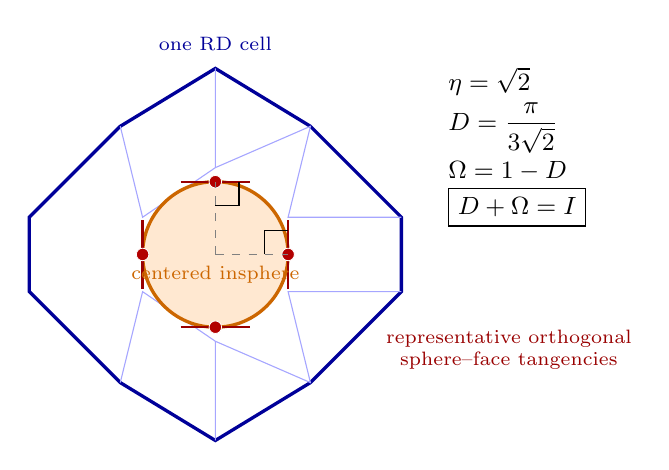
\begin{tikzpicture}[
  scale=1.05,
  every node/.style={font=\small},
  contact/.style={fill=red!70!black, draw=white, line width=.3pt}
]
\coordinate (O) at (0,0);
\coordinate (Ttop) at (0,.88);
\coordinate (TtopR) at (.42,.88);
\coordinate (Tright) at (.88,0);
\coordinate (TrightT) at (.88,.42);
\draw[very thick, blue!60!black]
  (0,2.25)--(1.15,1.55)--(2.25,.45)--(2.25,-.45)--
  (1.15,-1.55)--(0,-2.25)--(-1.15,-1.55)--(-2.25,-.45)--
  (-2.25,.45)--(-1.15,1.55)--cycle;
\draw[blue!35]
  (0,2.25)--(0,1.05)--(1.15,1.55)--(.88,.45)--(2.25,.45)
  (0,1.05)--(-.88,.45)--(-1.15,1.55)
  (0,-2.25)--(0,-1.05)--(1.15,-1.55)--(.88,-.45)--(2.25,-.45)
  (0,-1.05)--(-.88,-.45)--(-1.15,-1.55);
\fill[orange!18] (O) circle (.88);
\draw[very thick, orange!80!black] (O) circle (.88);
% Representative projected face planes tangent to the insphere.
\draw[red!60!black, thick] (-.42,.88)--(.42,.88);
\draw[red!60!black, thick] (-.42,-.88)--(.42,-.88);
\draw[red!60!black, thick] (.88,-.42)--(.88,.42);
\draw[red!60!black, thick] (-.88,-.42)--(-.88,.42);
\foreach \p in {(0,.88),(0,-.88),(.88,0),(-.88,0)}
  \node[contact,circle,inner sep=1.6pt] at \p {};
\draw[dashed, gray] (O)--(0,.88);
\draw[dashed, gray] (O)--(.88,0);
\draw pic[draw,angle radius=3mm] {right angle = O--Ttop--TtopR};
\draw pic[draw,angle radius=3mm] {right angle = O--Tright--TrightT};
\node[align=left, anchor=west] at (2.7,1.3)
  {\(\eta=\sqrt2\)\\[2pt]
   \(D=\dfrac{\pi}{3\sqrt2}\)\\[2pt]
   \(\Omega=1-D\)\\[2pt]
   \(\boxed{D+\Omega=I}\)};
\node[font=\scriptsize, text=orange!80!black] at (0,-.25)
  {centered insphere};
\node[font=\scriptsize, text=blue!60!black] at (0,2.55)
  {one RD cell};
\node[font=\scriptsize, text=red!60!black, align=center] at (3.55,-1.15)
  {representative orthogonal\\sphere--face tangencies};
\end{tikzpicture}
\caption{Coordinate presentation of the derived FCC/rhombic-dodecahedral
cell, its centered inscribed sphere, and representative orthogonal tangencies.
The sphere and cell boundary are distinct except at the tangency points.  The
drawing presents derived relational geometry; it is not a primitive external
lattice or background space.}
\label{fig:fcc-rd-cell}
\end{figure}

\Needspace{7\baselineskip}
\section{Runtime Accounting: Tick, Escapement, and Residual Growth}
\label{sec:05}
Section 4 supplied the static cell: the FCC/RD presentation, the filled share \(D\), the residual share \(\Omega\), and the static referent \(\operatorname{REF}(\xi)\). Section 5 asks what happens when that residual share is allowed to run.

The answer is not physical time yet. It is not a clock reading, not a rate in seconds, and not a dynamics in a background space. It is an internal accounting process: a residual register receives the same strictly positive share each cycle, carries the leftover forward, and posts a completed unit only when the account reaches one whole unit.

% LAYOUT_ONLY_GUARD:RUNTIME_IRRATIONALITY_LEADIN
\Needspace{14\baselineskip}
The running of the account is not an added iteration rule. Admitted existence has no licensed terminal book, and its book of licensed entries has no last entry; while admitted content stands, there must be a next closure-attempt in the order. At the base runtime layer, before any scheduling, physical-time, or observer-readout structure has been introduced, that renewed attempt has exactly one licensed representation: the base tick. The attempts therefore recur. There is no last tick. This recurrence does not depend on the irrationality of \(\Omega\) and would still hold even if a discharge settled exactly. The irrationality of

\begin{equation*}
\begin{adjustbox}{max width=\linewidth,center}
$\displaystyle
1-\frac{\pi}{3\sqrt{2}}
$
\end{adjustbox}
\end{equation*}
sharpens the internal runtime for the exact residual value used here. Recurrence is already forced by the no-terminal/no-last account and the tick-uniqueness result; irrationality does not make ticks recur. What irrationality adds is stricter: the internal residual account never settles exactly, so each recurring tick is a re-attempt at the same standing account, and the present residual determines the ledger tick history, in principle from an exact residual reading, rather than storing an archive.

That distinction matters. The paper now separates three things that ordinary language can easily blur:

\begin{itemize}
\item a \textbf{tick}, the base runtime event;
\item an \textbf{escapement}, the threshold-crossing event caused by some ticks but not all ticks;
\item a \textbf{cell}, the relational co-end created when an escapement posts a completed unit.
\end{itemize}
One cell is created per escapement, never per tick.

\Needspace{5\baselineskip}
\subsection{The Residual Register}
The runtime layer needs a place where the uncompleted share can be held. That object is the residual register \(S_{\mathrm{res}}\). It is a partial holding: when present, it holds a strictly positive residual; when no residual remains, the register is absent from the book. It is never a register containing zero.

The core runtime state is therefore minimal:

\begin{equation*}
\begin{adjustbox}{max width=\linewidth,center}
$\displaystyle
\operatorname{State}_{\mathrm{rt}}(k)
=
\big(S_{\mathrm{res}}(k)\big).
$
\end{adjustbox}
\end{equation*}
Here \(k\) is the update index of the running account. It is not physical time. The event index and physical-time index are kept distinct from it. In this section, the runtime book is only an internal account whose state can change; the bridge to measured time belongs later.

The residual is read against the unit account \(I=1\). If a current residual is present, its account ratio is

\begin{equation*}
\begin{adjustbox}{max width=\linewidth,center}
$\displaystyle
R_{\mathrm{acc}}
=
\frac{S_{\mathrm{res}}}{I}
=
S_{\mathrm{res}}
\qquad (I=1).
$
\end{adjustbox}
\end{equation*}
The equality on the right is numerical because the unit threshold is \(1\), but the meaning is not "a free decimal value." It is a unit-relative account standing: below one, exactly one, or above one. A sub-unit residual is not yet completed existence. A completed unit is the threshold at which the book must post.

\Needspace{5\baselineskip}
\subsection{The Cell Increment}
The residual share from Section 4 becomes the per-tick runtime increment:

\begin{equation*}
\begin{adjustbox}{max width=\linewidth,center}
$\displaystyle
\Omega_{\mathrm{cell}}^{\mathrm{slot}}
=
\omega_{\mathrm{cell}}
=
\Omega_{\mathrm{geom}}
=
\Omega_{\mathrm{pack}}
=
1-\frac{\pi}{3\sqrt{2}} .
$
\end{adjustbox}
\end{equation*}
% LAYOUT_ONLY_GUARD:RUNTIME_TYPED_ROLE_PARAGRAPH
\Needspace{11\baselineskip}
This equality carries one fixed value across two typed roles. The symbol \(\Omega_{\mathrm{geom}}\) names the normalized geometric residual share, while \(\omega_{\mathrm{cell}}\) names the equal feed supplied at each serviced tick. Neither symbol is the live state \(S_{\mathrm{res}}(K)\), which changes with \(K\). The identity is the licensed handoff from the static cell to the runtime register; it does not make \(\Omega\) a mass, a physical density, a measured unit, or an accumulated state.

The feed into the runtime register is an admission, not a transfer from another register. The cell-side residual share and the register-side entry in \(S_{\mathrm{res}}\) are two readings of one admitted share. No source register exists and nothing moves, so the transfer-conservation law is not being bypassed. On the static cell side, \(\Omega\) names the share not occupied by the filled portion of the cell. On the runtime side, repeated feeds of that fixed share change the live register state \(S_{\mathrm{res}}(K)\) toward the unit threshold; \(\Omega\) itself does not accumulate or vary with \(K\). When an escapement occurs, the completed unit posts. If the crossing overshoots the unit, the runtime residual is the positive carry beyond that posted unit; if the crossing is exact, the residual register is absent.

For a strictly positive cycle count \(x\), the accumulated input is

\begin{equation*}
\begin{adjustbox}{max width=\linewidth,center}
$\displaystyle
u_{\mathrm{tick}}(x)=x\Omega .
$
\end{adjustbox}
\end{equation*}
The notation

\begin{equation*}
\begin{adjustbox}{max width=\linewidth,center}
$\displaystyle
N_{\mathrm{tick}}(x)=\lfloor x\Omega\rfloor
$
\end{adjustbox}
\end{equation*}
must be read with care. Despite the glyph, it counts completed unit-account crossings: escapements. It is not the number of base ticks. If no crossing has occurred, the report is the absence of a posted event, not a held zero count.

\Needspace{5\baselineskip}
\subsection{Tick and Escapement}
A tick is the base runtime event. Each tick advances the residual account by \(\omega_{\mathrm{cell}}=\Omega\). Since \(0<\Omega<1\), one tick contributes less than the unit account \(I=1\) by itself. It completes a unit only when the standing residual already puts the updated account at or past the threshold.

An escapement is different. It occurs exactly when the updated residual reaches the unit threshold:

\begin{equation*}
\begin{adjustbox}{max width=\linewidth,center}
$\displaystyle
S_{\mathrm{res}}(k)\oplus\omega_{\mathrm{cell}}\succeq 1 .
$
\end{adjustbox}
\end{equation*}
The symbol \(\oplus\) here is the positive accumulation operation of the ledger, and \(\succeq\) is the positive-gap order against the unit account. The condition is a crossing condition, not a hidden equality-to-zero construction and not signed subtraction.

When the crossing occurs, one unit of existence has completed. Non-erasure then leaves no option for that completed unit to disappear as a non-entry. The book must post it, and because exactly one whole unit has completed, the posting is exactly

\begin{equation*}
\begin{adjustbox}{max width=\linewidth,center}
$\displaystyle
\Delta I=1 .
$
\end{adjustbox}
\end{equation*}
This value is not stipulated. It follows from account completion: one completed unit of existence posts one completed unit-token.

\Needspace{5\baselineskip}
\subsection{The Update Rule}
Given the recurring attempts, each serviced update has the transfer-side accounting form

\begin{equation*}
\begin{adjustbox}{max width=\linewidth,center}
$\displaystyle
S_{\mathrm{res}}(k+1)
=
S_{\mathrm{res}}(k)\oplus\omega_{\mathrm{cell}}\ominus[\mathrm{posting}] .
$
\end{adjustbox}
\end{equation*}
The notation \(\ominus\) does not introduce signed subtraction. If no posting occurs, the residual simply grows by \(\omega_{\mathrm{cell}}\). If a posting occurs, one whole unit is posted from the residual account as the completed-unit event count. The next residual is the unique positive remainder whose sum with that posted unit restores the accumulated amount. In runtime language, residual means unposted accumulation before threshold and positive overrun carried forward after an escapement. If the crossing is exact, the residual register leaves the book.

Thus every branch preserves the Section 2 discipline. The register either holds a strictly positive leftover below the unit or is absent. It never stores zero, and no negative residual is introduced.

The real-arithmetic closed form of the accounting identity is

\begin{equation*}
\begin{adjustbox}{max width=\linewidth,center}
$\displaystyle
S_{\mathrm{res}}(0)+K\omega_{\mathrm{cell}}
=
S_{\mathrm{res}}(K)+T_{\mathrm{rt}}(K)\cdot 1 ,
$
\end{adjustbox}
\end{equation*}
where \(T_{\mathrm{rt}}(K)\) is the count of completed unit-accounts by cycle \(K\). Equivalently,

\begin{equation*}
\begin{adjustbox}{max width=\linewidth,center}
$\displaystyle
T_{\mathrm{rt}}(K)
=
\left\lfloor S_{\mathrm{res}}(0)+K\omega_{\mathrm{cell}}\right\rfloor ,
\qquad
S_{\mathrm{res}}(K)
=
\operatorname{frac}\!\left(S_{\mathrm{res}}(0)+K\omega_{\mathrm{cell}}\right).
$
\end{adjustbox}
\end{equation*}
The floor counts completed units. The fractional part is the unitized residual ratio that remains, when a residual remains. The arithmetic is exact, but the ontology is still account completion, not free-floating real-number floor math.

% LAYOUT_ONLY_GUARD:EMPTY_HISTORY_START
\Needspace{7\baselineskip}
At the empty-history start, this reduces to the inherited \(N_{\mathrm{tick}}\) form:

\begin{equation*}
\begin{adjustbox}{max width=\linewidth,center}
$\displaystyle
T_{\mathrm{rt}}(K)=N_{\mathrm{tick}}(K),
\qquad
S_{\mathrm{res}}(K)=\operatorname{frac}(K\Omega).
$
\end{adjustbox}
\end{equation*}
\Needspace{5\baselineskip}
\subsection{The Escapement Staircase}
Because \(\Omega=1-\pi/(3\sqrt{2})\), the first few completions are not arbitrary. The exact inequalities give

\begin{equation*}
\begin{adjustbox}{max width=\linewidth,center}
$\displaystyle
N_{\mathrm{tick}}(3)\ \text{has no posted event},
\qquad
N_{\mathrm{tick}}(4)=1 .
$
\end{adjustbox}
\end{equation*}
Equivalently,

\begin{equation*}
\begin{adjustbox}{max width=\linewidth,center}
$\displaystyle
4\Omega=1+\varepsilon_4 .
$
\end{adjustbox}
\end{equation*}
More generally, the gaps between successive single-cell completions are exactly a \(\{3,4\}\) staircase:

\begin{equation*}
\begin{adjustbox}{max width=\linewidth,center}
$\displaystyle
\text{gaps}\in\{3,4\}
\Longleftrightarrow
\frac14<\Omega<\frac13
\Longleftrightarrow
2\sqrt{2}<\pi<\frac{9\sqrt{2}}{4}.
$
\end{adjustbox}
\end{equation*}
This is a runtime count statement. It is not a physical clock, not seconds, not a frequency measurement, and not the slower four-cell pooled clock. The four-cell \(\{26,27\}\) reading is fenced as a separate object. The single-cell staircase is the exact escapement pattern of this runtime account.

The long-run completion rate is also exact:

\begin{equation*}
\begin{adjustbox}{max width=\linewidth,center}
$\displaystyle
\lim_{x\to\infty}\frac{N_{\mathrm{tick}}(x)}{x}
=
\Omega ,
\qquad
\Omega-\frac1x
<
\frac{N_{\mathrm{tick}}(x)}{x}
\le
\Omega .
$
\end{adjustbox}
\end{equation*}
This is the only rate statement made here, and it remains an internal completion rate: completed unit-accounts per cycle. The limiting argument genuinely uses real analysis: the ratio is trapped between \(\Omega\) and \(\Omega-1/x\), and the width of that interval closes as \(x\) grows. It does not convert \(k\), \(x\), or \(K\) into physical time.

\Needspace{5\baselineskip}
\subsection{Cells Completed by Escapement}
When an escapement posts \(\Delta I=1\), one cell is completed as the opposite-side reading of the same non-erased transfer. The source-side reading is the unit leaving the residual account; the co-end reading is the \(+1\) cell. These are not two detached creations. They are one paired relational event read from two sides.

Therefore the cell count follows the escapement count:

\begin{equation*}
\begin{adjustbox}{max width=\linewidth,center}
$\displaystyle
\#\mathrm{cells}
=
\#\mathrm{escapements}
=
\lfloor x\Omega\rfloor
<
x .
$
\end{adjustbox}
\end{equation*}
This is the main distinction the section needs. The runtime does not generate one cell per base tick. It generates one cell per threshold crossing. Most ticks are only residual advances.

Each cell may carry its own residual, and that does not create a second existence. The cells remain one existence because each child is relationally connected to its origin as the \(+1\) co-end of the transfer that produced it. An unconnected cell would be a second existence and is excluded. The binding here is relational connectedness, not gravity, not a background coordinate adjacency, and not a later observer frame.

The cross-cell connective is also unpreferred at this layer. Every reading must be paired, so dangling half-links are forbidden. But no global orientation has yet been supplied that could privilege one cross-cell path over another. That global orientation belongs to the later observer construction. Section 5 only gives the dangling-free, unpreferred runtime connective.

One exact first-jump consequence is available. Because the exact inequality \(\pi>15\sqrt{2}/7\) fixes the relevant second-gap branch, the origin's second escapement and the first child's first escapement land together at tick \(8\). The population therefore jumps

\begin{equation*}
\begin{adjustbox}{max width=\linewidth,center}
$\displaystyle
2\longrightarrow 4
$
\end{adjustbox}
\end{equation*}
and skips a stable \(3\) at the first jump. This is a first-jump result only. It does not claim a general growth law, does not decide whether the four-cell system later couples, and does not introduce readout, clockhood, mass, energy, or physical time.

\Needspace{5\baselineskip}
\subsection{Boundary of the Section}
Section 5 has converted the static residual share \(\Omega\) into runtime accounting. It has supplied the residual register, the recurring-attempt theorem, the per-tick increment, the feed-admission articulation, the tick/escapement distinction, the forced unit posting, the update rule, the floor-sum account reading, the \(\{3,4\}\) staircase, the internal completion rate, and the first relational growth consequence.

It has not built physical time. It has not built clockhood. It has not read \(\Omega\) as mass or energy. It has not used gravity as a binding mechanism. It has not installed a background lattice-growth process. It has not assigned observer orientation, measurement, aperture, SI units, or empirical comparison. Those are later questions, and they must preserve the runtime accounting established here.

The section can fail in concrete ways. Exhibit a final licensed tick while admitted content still stands, and the recurrence theorem falls. Exhibit a runtime state that stores a zero residual, and the strict-positivity fence falls. Exhibit a lawful update in which the residual exceeds the unit without posting, and the bounded-residual theorem falls. Exhibit a crossing that does not force \(\Delta I=1\), and account completion fails. Exhibit a stable first population \(3\) under the exact \(\Omega\) arithmetic, and the first-jump result fails. Exhibit one cell per base tick rather than one per escapement, and the growth identity fails.


\Needspace{7\baselineskip}
\section{Aperture and Resolution}
\label{sec:06}
Section 5 showed that the runtime account does not stop: the residual account is repeatedly serviced, ticks recur, and escapements post completed units when the standing account crosses the unit threshold. Section 6 asks a different question. Given two relational histories, when is their difference large enough to be read as a resolved distinction?

Inside the theory, the issue is a floor: an action gap smaller than one resolution unit posts no resolved distinction. At and above one unit, completed units can be counted. This manuscript uses only that internal action/count structure. Possible translations into calibrated physical action or externally normalized resolution belong to later bridge work and are not part of the present derivation.

The internal count remains a count of completed distinguishability units.

\Needspace{5\baselineskip}
\subsection{Relational Histories}
The objects compared by the aperture layer are histories. A history is not a path through a pre-existing space. It is an admissible relational walk from one distinguishability event to another:

\begin{equation*}
\begin{adjustbox}{max width=\linewidth,center}
$\displaystyle
\mathcal{H}(A,B)
:=
\{\,w:\; w \text{ is an admissible relational walk from } A \text{ to } B\,\}.
$
\end{adjustbox}
\end{equation*}
If \(\gamma_1\in\mathcal{H}(A,B)\) and \(\gamma_2\in\mathcal{H}(B,C)\), the two histories may be chained,

\begin{equation*}
\begin{adjustbox}{max width=\linewidth,center}
$\displaystyle
\gamma_1\circ\gamma_2\in\mathcal{H}(A,C).
$
\end{adjustbox}
\end{equation*}
The empty history is the empty walk \(\varepsilon\). It is a walk identity for concatenation, not a zero object. That distinction matters because the aperture layer continues the same no-zero discipline used in Sections 1 and 2: absence, no increment, no difference, and no resolved distinction are typed predicates, never stored zero quantities.

\Needspace{5\baselineskip}
\subsection{Internal Action}
Over these histories the theory defines an internal action functional:

\begin{equation*}
\begin{adjustbox}{max width=\linewidth,center}
$\displaystyle
\mathcal{S}_\Phi:\mathcal{H}(A,B)\longrightarrow \mathcal{D}^{+}_{\mathrm{act}} .
$
\end{adjustbox}
\end{equation*}
For a non-empty history, \(\mathcal{S}_\Phi[\gamma]\) is a strictly positive internal action holding. Its defining structural property is concatenation additivity:

\begin{equation*}
\begin{adjustbox}{max width=\linewidth,center}
$\displaystyle
\mathcal{S}_\Phi[\gamma_1\circ\gamma_2]
=
\mathcal{S}_\Phi[\gamma_1]\oplus \mathcal{S}_\Phi[\gamma_2].
$
\end{adjustbox}
\end{equation*}
The operation \(\oplus\) is the positive composition already licensed for the quantity domain. Nothing here requires signed subtraction. The action assigned to a history is a single internal readout of that history; the order and relational structure remain in the history itself. The empty-history case is again predicate-like: \(\mathcal{S}_\Phi[\varepsilon]\) contributes no action increment, but it is not represented as a stored zero action.

\Needspace{5\baselineskip}
\subsection{The Resolution Unit}
An action readout becomes distinguishability only after the theory fixes a resolution unit. That unit is

\begin{equation*}
\begin{adjustbox}{max width=\linewidth,center}
$\displaystyle
u_\Phi\in\mathcal{D}^{+}_{\mathrm{act}},
\qquad
u_\Phi>0.
$
\end{adjustbox}
\end{equation*}
It is the internal action difference corresponding to one completed unit of distinguishability:

\begin{equation*}
\begin{adjustbox}{max width=\linewidth,center}
$\displaystyle
\Delta(\mathcal{S}_\Phi/u_\Phi)=1
\Longleftrightarrow
\Delta I=1.
$
\end{adjustbox}
\end{equation*}
Thus \(u_\Phi\) is unit-relative. If the action readout and the internal resolution unit are rescaled together, the distinguishability count does not change. The invariant is the one-unit threshold, not the printed size of the unit. This is the same pattern already used in the runtime account: the account is measured by completed units, not by treating a reporting scale as an object of nature.

\Needspace{5\baselineskip}
\subsection{The Action Gap}
For two histories \(\gamma_1,\gamma_2\), the action gap is not a signed subtraction. The theory compares their internal action readouts by the positive-gap order. If one action strictly exceeds the other, there is a unique strictly positive excess \(e\) satisfying

\begin{equation*}
\begin{adjustbox}{max width=\linewidth,center}
$\displaystyle
\text{smaller}\oplus e=\text{larger}.
$
\end{adjustbox}
\end{equation*}
The gap is then recorded as a which-side tag together with a positive-excess readout:

\begin{equation*}
\begin{adjustbox}{max width=\linewidth,center}
$\displaystyle
g_\Phi(\gamma_1,\gamma_2):=(\sigma, |g_\Phi|),
\qquad
|g_\Phi|:=\frac{e}{u_\Phi}.
$
\end{adjustbox}
\end{equation*}
% LAYOUT_ONLY_GUARD:ACTION_GAP_TAG_PARAGRAPH
\Needspace{12\baselineskip}
The tag \(\sigma\) records only which history carries the larger action. It is a history-side tag in this comparison, not a four-cell observer standpoint, not spatial direction, and not the later observer-readout structure. At this layer, two histories give only a comparative side and a positive excess. The readout \(|g_\Phi|\) is that positive excess in \(u_\Phi\) units, taken only at coefficient readout; it is not a standalone primitive quantity or measured size. If the two action readouts match, the result is a paired-balance predicate: no excess exists. The theory does not store a zero-valued gap.

This is the aperture layer's basic comparison object. It is dimensionless, unit-relative, and internal. It is not a distance, not a coordinate, not a physical phase by itself, and not yet a comparison with experiment.

\Needspace{5\baselineskip}
\subsection{The Resolution Floor}
The floor is the first theorem of the section. A sub-unit gap does not post a resolved distinction:

\begin{equation*}
\begin{adjustbox}{max width=\linewidth,center}
$\displaystyle
|g_\Phi|<1
\Longrightarrow
\text{no resolved distinction is on record}.
$
\end{adjustbox}
\end{equation*}
That sentence should be read literally. Below the unit threshold there is an open account, not a zero count. Nothing has completed, so nothing posts. When the gap reaches one full unit, a unit of distinguishability has completed; by non-erasure it must be accounted, and the posting is forced:

\begin{equation*}
\begin{adjustbox}{max width=\linewidth,center}
$\displaystyle
\Delta I=1.
$
\end{adjustbox}
\end{equation*}
The resulting count is the number of completed unit crossings. The reason is purely discrete: the gap \(|g_\Phi|\) is the positive excess read in \(u_\Phi\)-units; only whole unit crossings are completed distinguishability units; and any remaining fractional part is still an open account. The account can therefore record exactly the largest whole number of completed crossings not exceeding \(|g_\Phi|\):

\begin{equation*}
\begin{adjustbox}{max width=\linewidth,center}
$\displaystyle
I(\gamma_1,\gamma_2)=\big\lfloor |g_\Phi| \big\rfloor .
$
\end{adjustbox}
\end{equation*}
The floor symbol is an external completed-crossing readout. Internally, the object is the standing gap and the account discipline around it. At base saturation, \(|g_\Phi|=1\), the same structure re-earns the first count:

\begin{equation*}
\begin{adjustbox}{max width=\linewidth,center}
$\displaystyle
I\big|_{|g_\Phi|=1}=1.
$
\end{adjustbox}
\end{equation*}
This does not ground the first count of Section 1. It reproduces it downstream at the aperture layer: one completed distinguishability unit reads as one.

\Needspace{5\baselineskip}
\subsection{Relative Phase}
The gap also supplies a relative coherence-phase record. Because \(g_\Phi\) is the ordered pair \((\sigma,|g_\Phi|)\), rather than a signed scalar, the record preserves the orientation tag and the phase magnitude as separate typed components:

\begin{equation*}
\begin{adjustbox}{max width=\linewidth,center}
$\displaystyle
\left(
\sigma,\;
\left[2\pi|g_\Phi|\right]_{2\pi}
\right).
$
\end{adjustbox}
\end{equation*}
The brackets denote the phase-magnitude class modulo \(2\pi\); they do not act on \(\sigma\).

% LAYOUT_ONLY_GUARD:RELATIVE_PHASE_FIREWALL
\Needspace{10\baselineskip}
Only relative phase is contentful here. The phase is a reading of a gap between histories, so an absolute phase of a single isolated history is not an admitted object. A uniform offset changes no action gap and no completed-crossing count. At this generic layer \(\sigma\) remains a non-arithmetic orientation tag: it is carried beside the phase magnitude and is neither multiplied nor treated as a signed holding.

The full turn \(2\pi\) is consumed from the earlier closure result. It is not re-derived in this section. Each completed \(2\pi\) closure corresponds to one completed distinguishability unit, so the closure count is again

\begin{equation*}
\begin{adjustbox}{max width=\linewidth,center}
$\displaystyle
I=\big\lfloor |g_\Phi|\big\rfloor .
$
\end{adjustbox}
\end{equation*}
This generic tag is distinct from the later lepton-specific orientation realization. In the promoted spectral theorem, orientation is explicitly realized as a numerical label \(\sigma\in\{+1,-1\}\); only there are expressions such as \(\exp(i\sigma\Phi_o)\) licensed. The later numerical realization does not retroactively turn the generic Section 6 tag into an arithmetic sign.

\Needspace{5\baselineskip}
\subsection{Boundary of the Section}
Section 6 supplies the internal resolution layer: relational histories, internal action, the internal resolution unit, the oriented action-gap record, the resolution floor, the completed-crossing count, and the relative-phase reading. It introduces no measured units and no external calibration.

The section can lose in concrete ways. Exhibit a persistent resolved distinction below the unit floor, and the floor fails. Exhibit a stored zero gap or zero count inside the resolution layer, and the no-zero discipline fails. Treat the generic orientation tag as an arithmetic sign, and the pair typing fails. Treat an absolute phase as contentful, and the relative-phase discipline fails.


\Needspace{7\baselineskip}
\section{Closure and Junction Contracts}
\label{sec:07}
Section 6 supplied the retained internal aperture layer: histories, internal action, the resolution unit, the action gap, the completed-crossing count, and the oriented relative-phase record. It ended at a seam. The gap has a discrete side, carried as a side or facing of a completed posting, while its generic phase reading keeps the non-arithmetic orientation tag separate from the phase magnitude.

Section 7 closes that seam at the internal level. The task is not yet physical time, physical energy, a calibrated observer report, or a prediction. The task is narrower: say how completed unit-accounts are counted, how completed closures are paired with those counts, how service cost is typed, and when the closure account is silent.

\Needspace{5\baselineskip}
\subsection{The Internal Completion Rate}
The runtime account already has a completed-unit counter:

\begin{equation*}
\begin{adjustbox}{max width=\linewidth,center}
$\displaystyle
N_{\mathrm{tick}}(x)=\lfloor x\Omega\rfloor .
$
\end{adjustbox}
\end{equation*}
% LAYOUT_ONLY_GUARD:INTERNAL_COMPLETION_RATE
\Needspace{12\baselineskip}
The name must be read with the Section 5 discipline intact. This is not the number of base ticks. It is the number of completed unit-account postings by cycle \(x\), each posting being a completed unit \(I=1\). For a window \([x_1,x_2]\) of the discrete update index, with \(x_1<x_2\), the internal completion-rate object is

\begin{equation*}
\begin{adjustbox}{max width=\linewidth,center}
$\displaystyle
r_{\mathrm{int}}(x_1,x_2)
=
\frac{N_{\mathrm{tick}}(x_2)\ominus N_{\mathrm{tick}}(x_1)}
{x_2\ominus x_1}.
$
\end{adjustbox}
\end{equation*}
The numerator is the completed-count increment in the window. It is not signed subtraction. It is the positive count of completed postings when completed postings are present, and the open-account predicate when no completed posting is present. The denominator is the positive cycle count of the window. Thus \(r_{\mathrm{int}}\) is a discrete completion density per update cycle, not a derivative and not a rate in physical time.

The long-run readout of this object is inherited from the runtime account:

\begin{equation*}
\begin{adjustbox}{max width=\linewidth,center}
$\displaystyle
\lim_{x\to\infty}\frac{N_{\mathrm{tick}}(x)}{x}=\Omega .
$
\end{adjustbox}
\end{equation*}
This limit is not re-proved here, and it is not used as a bridge calibration. It says only that the internal completed-unit density has the already established bounded long-run value \(\Omega\). Since each completed unit-account is also one completed \(2\pi\) closure, the same count can be read from the closure side. That still does not identify the internal count density with a physical phase rate.

\Needspace{5\baselineskip}
\subsection{The Junction Contract}
Before an identity can be claimed, the section has to separate the obligations. There are four internal obligations and one bridge boundary.

First, each forced completed-unit posting must correspond to the \(2\pi\) closure of that same completion. Second, the tick-side and closure-side counts must agree over the same window. Third, the completed closure must carry one service burden, not two. Fourth, the orientation carried by the gap must be the orientation carried by the posting; it cannot be recovered afterward from a continuous phase reading.

The bridge boundary is different. It concerns physical time, physical energy, calibration, prediction, and the later readout layer. None of those are built by the internal junction. The internal section may prove a count identity and a completion identity. It may not turn those into a physical-time law.

\Needspace{5\baselineskip}
\subsection{Orientation Before Continuous Readout}
The posting order is discrete. The internal structure first has oriented closures, then completed postings, and then the count or rate read from those postings. A continuous phase representation may later read that structure, but it is not an input to the posting order.

The orientation label \(\sigma\) therefore has a fixed role. It tells which side or facing of the paired posting is being read. It is not a signed internal quantity, not a negative amount, and not a scalar recovered from cost or phase. Two completions with the same magnitude but opposite facing can have the same continuous phase reading; the phase reading alone therefore cannot recover \(\sigma\).

This is why the bridge-facing phase account is constrained before it is used. Any later continuous representation must consume the discrete postings, counts, and carried orientation. It cannot replace them.

\Needspace{5\baselineskip}
\subsection{Ticks and Closures}
The first internal obligation is the tick-closure correspondence. A completed unit-account produces a forced posting; that same completed unit is read as a completed \(2\pi\) closure. The map is one-to-one because it is indexed by the same completed unit. A tick-side completion without a closure, or a closure without the corresponding completion, would break the account.

The second obligation follows by restricting that correspondence to a window. Over \([x_1,x_2]\),

\begin{equation*}
\begin{adjustbox}{max width=\linewidth,center}
$\displaystyle
\Delta N_{\mathrm{tick}}(x_1,x_2)
=
\Delta I_{\mathrm{closure}}(x_1,x_2).
$
\end{adjustbox}
\end{equation*}
Dividing both sides by the same positive cycle-window count gives the internal equality

\begin{equation*}
\begin{adjustbox}{max width=\linewidth,center}
$\displaystyle
r_{\mathrm{int}}(x_1,x_2)=r_{\mathrm{closure}}(x_1,x_2).
$
\end{adjustbox}
\end{equation*}
The equality is exact at the internal count level. It is not obtained from the long-run value \(\Omega\), not from a physical-time calibration, and not from an external phase-rate law. The count equality comes first; any calibrated bridge reading must come later and preserve that dependency order.

\Needspace{5\baselineskip}
\subsection{Service Cost}
The third obligation is service. A completed closure carries one service/completion burden. For a distinction \(\gamma\),

\begin{equation*}
\begin{adjustbox}{max width=\linewidth,center}
$\displaystyle
\operatorname{cost}[\gamma]\in \mathcal{D}_{+},
\qquad
\operatorname{cost}[\gamma]
=
\text{one per-unit service burden per completed closure of }\gamma .
$
\end{adjustbox}
\end{equation*}
The cost is indexed by the completed closure count \(I(\gamma)\) and measured against the internal unit \(u_\Phi\). It types the burden of completion. It is not merely the count itself, and it is not physical energy.

The cost is strictly positive when a completion has occurred. If no completion has occurred, no service has been posted; that is the open-account predicate, not a stored value \(0\). The carried orientation remains separate. The value of the service burden is blind to \(\sigma\), but \(\sigma\) is not erased and not recovered from the service value.

\Needspace{5\baselineskip}
\subsection{From Narrowing to Identity}
The forced posting and the \(2\pi\) closure are already tied to the same completed unit. That establishes a narrowing: the completion is not two independently completing processes, and not two independently serviced processes. There is one forced completed unit, one count increment, one service burden, and the orientation is carried through both readings.

That narrowing is not yet the identity. It still permits a weaker rival description: two relations that always co-complete, always share one count, and always share one service. Section 7 has to rule out that rival description without assuming the answer.

The identity proof has two steps.

% LAYOUT_ONLY_GUARD:CLOSURE_STATE_UPDATE_PARAGRAPH
\Needspace{14\baselineskip}
First, the completion has two statement positions. On the result side, the residual is resolved into the forced completed-unit output. On the state side, the accumulated completion state is updated. The tick-closure correspondence articulates these two positions: the forced result is carried into the closure-side state update. The result is singular, the state update is singular, and the service burden is singular. Therefore any account that tries to make a second process by adding a second result, a second state update, a second service burden, or a third statement position has no licensed role left to occupy.

Second, the only remaining rival is weaker still. It claims two relations while sharing all roles and registering no second result, no second state update, no second service, no different orientation facing, no different paired record, no different licensed operation, and no later formal consequence. In this framework, that is not a hidden second relation. Existence is admitted only as relational distinguishability. A second admitted token must have an admitted relational difference. If every admitted mark is the same, the supposed second token is duplicate naming of one relation.

Thus the update-side completion and the closure-side completion are one internal completion relation-token read two ways. The theorem proves only this internal, pre-readout identity. It does not prove physical time, physical energy, prediction, or any calibrated bridge claim.

The resulting status is correspondingly narrow. The internal identity is established; the bridge-facing layer remains deferred. Physical time, physical energy, calibration, prediction, and the later observer-system reading remain outside this section.

\Needspace{5\baselineskip}
\subsection{The G-Operation and Complete Closure}
The section can now state the closure operation. The symbol \(G\) is used here by role, not by value. It is the system-level bookkeeping operation that reconciles what remains unpaired in the system account. The residual register is consumed here only as a typed category. The rule for its quantitative content is not derived here.

The \(G\)-operation pairs the unpaired records under the balance discipline. Complete system closure, or \(G\)-silence, is the condition in which no unpaired system-level residue remains:

\begin{equation*}
\begin{adjustbox}{max width=\linewidth,center}
$\displaystyle
G\vert_{\mathrm{self\text{-}coupled}}=0.
$
\end{adjustbox}
\end{equation*}
The displayed \(0\) is an absence marker: nothing is left for \(G\) to book. It is not the value \(I=0\), not a stored zero residual, and not annihilation. The existents persist paired and balanced. Complete closure removes the unpaired residue, not the admitted existents.

This definition also fences the section. It gives an operation and a closure condition. It assigns no value to \(G\), derives no dynamics of reaching closure, defines no \(\Omega\), and makes no physical-gravity claim.

\Needspace{5\baselineskip}
\subsection{Driven Dynamics Do Not Reach Complete Closure}
The final result is a no-go theorem for the driven regime. When a residual register is present, it is a strictly positive typed holding. When a discharge empties the register, the register leaves the book; it is not cleared to a stored zero value. Under driven cycling, a strictly positive feed is produced each cycle. A completion can discharge the current register, but the next cycle re-populates it.

Therefore register-absence is at most transient under continued driving. Complete system closure requires sustained register-absence, so driven dynamics do not reach complete closure. Complete closure requires forcing-cessation: the strictly positive feed must cease. It is not achieved by reducing a residual to \(S_{\mathrm{res}}=0\), since that zero state is not a licensed internal object.

The proof is not a geometry-value proof. The values \(D\), \(\Omega\), and \(\omega_{\mathrm{cell}}\) belong to the transitive runtime foundation, but the no-go uses only the strict-positivity type and non-erasure. The driver is persistence of admitted existence, not a pressure variable and not a physical force. The theorem also does not supply the positive mechanism by which forcing ceases. It proves the no-go and the necessary condition only.

\Needspace{5\baselineskip}
\subsection{Boundary of the Section}
Section 7 establishes the internal closure and junction account. It defines the internal completion-rate object, records the junction obligations, fixes orientation before continuous readout, proves the tick-closure and internal rate equalities, types service cost, proves the internal update-closure identity, defines the \(G\)-operation and complete-closure condition, and proves that driven dynamics do not reach complete closure without forcing-cessation.

It does not build physical time, physical energy, calibrated mass, gravity, empirical prediction, or observer-system measurement. It also does not assign a value to \(G\), derive the residual-register rule, or derive the positive dynamics by which forcing ceases.

This section can lose in specific ways. Exhibit a stored zero rate, zero service, or zero residual inside the internal account, and the typing fails. Exhibit a tick-side completion without the corresponding closure, or a closure without the corresponding completed unit, and the tick-closure map fails. Exhibit an internal rate equality that depends on physical-time calibration rather than count equality, and the dependency order fails. Exhibit a service burden that is physical energy rather than pre-physical completion burden, and the cost typing fails. Exhibit a second admitted relational mark that survives the identity proof, and the internal identity fails. Exhibit complete closure by erasing existents or by setting a residual to zero, and the non-erasure discipline fails. Exhibit sustained complete closure under continued strictly positive driving, and the no-go theorem fails.


\Needspace{7\baselineskip}
\section{Observer and Readout Architecture}
\label{sec:08}
Section 7 closed the internal junction account. It proved the internal update-closure identity, fixed the closure-side status, and stopped before observer-system readout. Section 8 begins on the other side of that boundary. Its task is not to import measured physics. Its task is to define what a readout locus is, how completed internal records become available to that locus, how those registrations function as a clock, and how completed closure extent becomes available as a time readout without changing the internal book.

The dependency direction is one-way. The readout layer consumes the completed internal record; it does not ground, reopen, or edit it. The word "observer" is therefore not a psychological word here. It names a relational role: the standpoint through which already resolved distinctions are available for reading.

\Needspace{5\baselineskip}
\subsection{The Readout Locus}
The first object is the readout locus \(L\). A locus is a relational standpoint at an internal resolution scale. Its content is the set of already resolved completed updates distinguishable at that scale:

\begin{equation*}
\begin{adjustbox}{max width=\linewidth,center}
$\displaystyle
\mathcal{D}(L)=\{u:\operatorname{reg}(L,u)\}.
$
\end{adjustbox}
\end{equation*}
% LAYOUT_ONLY_GUARD:REGISTERED_ELEMENT_PARAGRAPH
\Needspace{10\baselineskip}
The elements \(u\) are completed internal updates. They are registrable only after the internal resolution condition has been met; below that floor there is no registered object, not a stored zero value. Each registered element still carries its orientation. The locus does not create those distinctions, does not resolve them, and does not duplicate the aperture that resolved them. It only makes already resolved content available on the readout side.

This first set has no order. It is a membership surface: what is available at \(L\), not what came first, what follows, how much time has elapsed, or what physical rate is being measured. Those are later structures.

\Needspace{5\baselineskip}
\subsection{Registration}
Registration is the relation that populates the readout set. For a locus \(L\) and an already resolved update \(u\), the statement

\begin{equation*}
\begin{adjustbox}{max width=\linewidth,center}
$\displaystyle
\operatorname{reg}(L,u)
$
\end{adjustbox}
\end{equation*}
means that \(u\) is available at \(L\). Equivalently, \(u\in\mathcal{D}(L)\). This is a yes-or-no membership relation. It carries the orientation of \(u\), but it does not impose a sequence, compare positions, assign a duration, create a history of registrations, or turn the set into an ordered measure.

The distinction matters because a registration relation can be mistaken for measurement. It is not measurement in the later physical sense. It is availability of already resolved relational content at a locus. The internal structure has already done the resolving; registration reads it.

\Needspace{5\baselineskip}
\subsection{The Reference Role}
A distinguishable reading also needs a reference. For an existent or system \(X\) at a level \(\ell\), the observer/reference role may be written as

\begin{equation*}
\begin{adjustbox}{max width=\linewidth,center}
$\displaystyle
\operatorname{Obs}(X,\ell).
$
\end{adjustbox}
\end{equation*}
The role holds when \(X\) occupies a readout standpoint, supplies the relational reference relative to which registered content is distinguishable, and thereby makes a distinguishable readout available at that level. The reference is not a background frame and not a privileged object. It is a relation. A registered state is distinguishable from the standpoint that reads it.

This is the sense in which observerhood induces readout asymmetry. The observer does not create distinguishability. The distinguishability is primitive and the relevant completion has already been resolved. By occupying the reference role, \(X\) selects which oriented side is read as reference. The resulting asymmetry is an orientation selection, not a signed amount and not an act of creation.

The role is independent of a fixed cell count. One cell may occupy the standpoint. Without a second registered state there is no realized distinction to read against it; with more registered states there is more distinguishable content. The role supplies the reference condition, not a cell-number theorem.

\Needspace{5\baselineskip}
\subsection{Clockhood}
The unordered set \(\mathcal{D}(L)\) is still not a clock. Clockhood is a role in which registered content is read as an ordered measure. It requires three ingredients.

First, there must be a succession, inherited from the completed-closure count. Second, there must be a relational comparison standard against which that succession is read. Third, the locus reads the succession against the standard as a relative, pre-metric ordered measure.

The order therefore lives in the reading, not in the set. The set remains unordered; registration remains membership. A wristwatch, recurrence, heartbeat, or astronomical cycle is clock-like only when it occupies this role. Nothing is inherently a clock.

The comparison standard is relational. It is not a background grid, a privileged frame, a fixed external coordinate system, or an absolute clock. A recurrence may serve, but a second recurrence is not required; a single relational comparison baseline can supply the standard. Clockhood gives readable order. It still gives no physical unit, no calibrated time, no measured rate, and no prediction.

\Needspace{5\baselineskip}
\subsection{The Time Readout}
Through clockhood, the locus reads the inherited succession of registered completions against its relational comparison standard. Clockhood creates neither the completions nor their geometry. The time readout adds the per-closure extent. Each completed closure carries the dimensionless base extent

\begin{equation*}
\begin{adjustbox}{max width=\linewidth,center}
$\displaystyle
t_{\mathrm{base}}=2\pi .
$
\end{adjustbox}
\end{equation*}
Thus the time readout \(\mathrm{t}(L)\) is the locus reading its registered completed closures as carrying that per-closure extent. In closure units, it is the completed-closure count together with \(2\pi\) of extent per closure:

\begin{equation*}
\begin{adjustbox}{max width=\linewidth,center}
$\displaystyle
\mathrm{t}(L)=I\,t_{\mathrm{base}}.
$
\end{adjustbox}
\end{equation*}
This is why the time readout is not merely clockhood renamed. Clockhood supplies readable order; \(\mathrm{t}(L)\) binds the \(2\pi\) extent to each completed closure. The result is dimensionless, metric-free, and not yet calibrated into seconds or any other observer-scale unit. The later calibration relation is only a pointer at this stage; it is not folded into the readout.

\Needspace{5\baselineskip}
\subsection{Book-Energy Record}
Separately from the time readout, the established bookkeeping coefficient and channel-route count give the internal book-energy record

\begin{equation*}
\begin{adjustbox}{max width=\linewidth,center}
$\displaystyle
\mathrm{Cap}=c^{\otimes 2}=9,
\qquad
E=m\cdot \mathrm{Cap}=\frac{9}{2\pi}.
$
\end{adjustbox}
\end{equation*}
Here \(m\) is the active bookkeeping coefficient used in this expression. The expression is the channel-distribution image of that coefficient across the forced channel-route count. The symbol \(c\) in \(\mathrm{Cap}=c^{\otimes 2}\) is a channel-count factor, not the measured speed of light. The value \(9\) is the channel-route count, not a physical velocity squared. No physical rate or calibrated energy law is inferred from this internal record.

\Needspace{5\baselineskip}
\subsection{Structural Completion and Prediction Boundary}
At this point the observer/readout stack has an internal structural account of its source record, readout locus, registration, reference role, clock target, closure extent, and dependency direction. External calibration and comparison remain deferred.

That status does not unlock measured relativity, Lorentz recovery, time dilation, measured rates, empirical prediction, or gravity. The section therefore records internal structural completeness while refusing the measured-physics unlock.

The prediction layer is opened only procedurally. Later work must first derive the theory's own comparison-law analogues and only then compare externally. A measured prediction remains inadmissible until the relevant comparison law and measured bridge conditions have been supplied. The internal update-closure identity from Section 7 is available as internal theorem ground, but it cannot be converted into physical readout, empirical comparison, or prediction by this section.

\Needspace{5\baselineskip}
\subsection{Boundary of the Section}
Section 8 constructs the observer/readout architecture. It defines the readout locus, registration relation, observer/reference role, clockhood reading of inherited succession, closure-unit time readout, and the separately established internal book-energy record. It opens external calibration and prediction only as ordered future obligations.

It does not import measured time, assign SI units as fundamental, derive a measured mass-energy law, derive Lorentz recovery, derive gravity, produce a pre-comparison output, or claim empirical success.

This layer can also lose, and says how. Exhibit a readout locus that creates rather than consumes distinguishability, and the locus definition fails. Exhibit registration that orders the set, and the registration definition fails. Exhibit a clock without a relational comparison standard, and clockhood fails. Exhibit a time readout without \(2\pi\) per closure, and the time readout fails. Treat the internal book-energy record as a calibrated physical law, and its scope fence fails. Exhibit a measured prediction before the internally derived comparison law and measured comparison conditions exist, and the prediction boundary fails.


\Needspace{7\baselineskip}
\section{Recovery and Presentation Discipline}
\label{sec:09}
Section 8 established the observer/reference role, clockhood, the closure-unit time readout, the internal book-energy record, and the boundary between theory-native structure and calibrated reports. Section 9 fixes the discipline that governs every later presentation. A derived expression may be displayed, rendered, or compared only without erasing the relational record from which it came.

The direction remains one-way:

\begin{equation*}
\begin{adjustbox}{max width=\linewidth,center}
$\displaystyle
\text{admitted relational ground}
\longrightarrow
\text{typed readout}
\longrightarrow
\text{rendered presentation}.
$
\end{adjustbox}
\end{equation*}
A presentation may report an established object. It may not become the ground that establishes that object.

% LAYOUT_ONLY_HEADING_GUARD:RECORDED_CONSTRUCTION_SEQUENCE
\Needspace{20\baselineskip}
\subsection{Recorded Construction Before Rendering}
Let \(R\) be an already-established observer-local readout and let

\begin{equation*}
\begin{adjustbox}{max width=\linewidth,center}
$\displaystyle
\operatorname{Rec}_O(R)
$
\end{adjustbox}
\end{equation*}
% LAYOUT_ONLY_GUARD:RENDERED_PRESENTATION_LEADIN
\Needspace{9\baselineskip}
be its governing construction record. The record identifies the upstream objects, counts, tags, and operations that make the readout what it is. A rendered presentation

\begin{equation*}
\begin{adjustbox}{max width=\linewidth,center}
$\displaystyle
Y=\operatorname{Render}_O(R;\mathcal A)
$
\end{adjustbox}
\end{equation*}
is therefore not admitted merely because \(Y\) is a well-formed scalar or exact symbolic expression. The originating record must remain available.

This condition preserves the distinction between exact representation and primitive admission. A downstream expression may be rational, irrational, transcendental, signed, continuous, or complex when its owning result licenses that domain. Its number class neither supplies nor defeats its scientific authority. What matters is the upstream derivation, the declared type, the domain guards, and the retained construction record.

\Needspace{5\baselineskip}
\subsection{The Recoverable Count Index}
For a promoted readout \(R\), let

\begin{equation*}
\begin{adjustbox}{max width=\linewidth,center}
$\displaystyle
\operatorname{Idx}_O(R)
:=
\pi_{\mathrm{idx}}
\!\left(
\operatorname{Rec}_O(R)
\right)
$
\end{adjustbox}
\end{equation*}
be the finite count-index data extracted from its construction record. The recoverable count-index package is

\begin{equation*}
\begin{adjustbox}{max width=\linewidth,center}
$\displaystyle
\boxed{
\operatorname{RCI}_O(R)
:=
\left(
\operatorname{Idx}_O(R),
\operatorname{Rec}_O(R)
\right).
}
$
\end{adjustbox}
\end{equation*}
This package is not a scalar and not a physical magnitude. It carries both the count data and the construction that types those data.

A rendered presentation is count-index admissible only when

\begin{equation*}
\begin{adjustbox}{max width=\linewidth,center}
$\displaystyle
\boxed{
\operatorname{Recover}_O
\left(
Y,
\operatorname{Rec}_O(R)
\right)
=
\operatorname{RCI}_O(R).
}
$
\end{adjustbox}
\end{equation*}
Equivalently, recovery must preserve both projections:

\begin{equation*}
\begin{adjustbox}{max width=\linewidth,center}
$\displaystyle
\pi_1
\operatorname{Recover}_O
\left(
Y,
\operatorname{Rec}_O(R)
\right)
=
\operatorname{Idx}_O(R),
$
\end{adjustbox}
\end{equation*}
\begin{equation*}
\begin{adjustbox}{max width=\linewidth,center}
$\displaystyle
\pi_2
\operatorname{Recover}_O
\left(
Y,
\operatorname{Rec}_O(R)
\right)
=
\operatorname{Rec}_O(R).
$
\end{adjustbox}
\end{equation*}
Recovering a numeral from \(Y\) alone is insufficient. The scalar may be many-to-one, convention-dependent, or incapable of distinguishing the construction that produced it. The admissible witness is recorded-construction recovery, not bare scalar inversion.

This is a scoped rule for rendered observer-local readouts. It is not a new universal demand that every derived quantity possess one common inverse map. Definitions, exact identities, role witnesses, and representation witnesses retain the proof forms supplied by their owning results.

\Needspace{5\baselineskip}
\subsection{Recovery Before Later Operations}
% LAYOUT_ONLY_GUARD:RECOVERY_OPERATION_SEQUENCE
\Needspace{18\baselineskip}
Suppose

\begin{equation*}
\begin{adjustbox}{max width=\linewidth,center}
$\displaystyle
Y_i
=
\operatorname{Render}_O(R_i;\mathcal A_i),
\qquad
i=1,\ldots,n,
$
\end{adjustbox}
\end{equation*}
% LAYOUT_ONLY_GUARD:LATER_OPERATION_SEQUENCE
\Needspace{10\baselineskip}
are rendered reports of promoted readouts. A later operation

\begin{equation*}
\begin{adjustbox}{max width=\linewidth,center}
$\displaystyle
Z=\Phi(Y_1,\ldots,Y_n)
$
\end{adjustbox}
\end{equation*}
may compare, ratio, normalize, rescale, or otherwise combine those reports only after each input has passed recovery.

% LAYOUT_ONLY_GUARD:OPERATION_RECORD_LEADIN
\Needspace{12\baselineskip}
The operation must carry its own record,

\begin{equation*}
\begin{adjustbox}{max width=\linewidth,center}
$\displaystyle
\operatorname{OpRec}_O
\left(
\Phi;Y_1,\ldots,Y_n
\right),
$
\end{adjustbox}
\end{equation*}
including the operation, the source readouts, their construction records, and any admitted reporting standards. Admissibility requires

\begin{equation*}
\begin{adjustbox}{max width=\linewidth,center}
$\displaystyle
\operatorname{Use}^{\Phi}_O
(Y_1,\ldots,Y_n)
\downarrow
\Longrightarrow
\bigwedge_{i=1}^{n}
\operatorname{RCIAdm}_O(Y_i;R_i)
\downarrow,
$
\end{adjustbox}
\end{equation*}
and an operation-level recovery map satisfying

\begin{equation*}
\begin{adjustbox}{max width=\linewidth,center}
$\displaystyle
\boxed{
\operatorname{Recover}^{\Phi}_O
\left(
Z,
\operatorname{OpRec}_O
\left(
\Phi;Y_1,\ldots,Y_n
\right)
\right)
=
\left(
\operatorname{RCI}_O(R_1),
\ldots,
\operatorname{RCI}_O(R_n)
\right).
}
$
\end{adjustbox}
\end{equation*}
If one source package is not recoverable, the later operation is blocked. Smooth algebra may not erase the discrete account that licensed its inputs.

\Needspace{5\baselineskip}
\subsection{Reporting Standards Do Not Change Content}
A reporting standard is admitted separately from the object being reported. Under a common positive change of unit,

\begin{equation*}
\begin{adjustbox}{max width=\linewidth,center}
$\displaystyle
u'=\kappa u,
\qquad
q'=\kappa^{-1}q,
\qquad
\kappa>0,
$
\end{adjustbox}
\end{equation*}
so that

\begin{equation*}
\begin{adjustbox}{max width=\linewidth,center}
$\displaystyle
q'u'=qu.
$
\end{adjustbox}
\end{equation*}
The coefficient changes; the represented object and its recovery package do not. Unit choice is therefore presentation data, not ontological ground. A valid rescaling must preserve the source record and the comparison relation that licensed the report.

\Needspace{5\baselineskip}
\subsection{Organizational Displays}
The same boundary governs the paper's bookkeeping arrays. Their entries are independently established before being grouped for readability. A row, column, adjacency, or vacant display position supplies no scientific premise. In particular, the arrays used here license no matrix multiplication, row operation, column operation, determinant, inverse, eigenvalue, tensor operation, or linear-operator interpretation.

The logical direction is

\begin{equation*}
\begin{adjustbox}{max width=\linewidth,center}
$\displaystyle
\text{independent scientific ground}
\longrightarrow
\text{typed quantities and relations}
\longrightarrow
\text{organized display},
$
\end{adjustbox}
\end{equation*}
never the reverse. If a future result uses an algebraic matrix operation, the underlying algebraic object, domain, operation, and interpretation must first be established independently.

Section 9 establishes recorded-construction recovery, recovery before later operations, the conventional status of reporting units, and the non-inferential role of organizational displays. It does not render a new physical quantity, assign a matrix position, derive a calibration constant, perform a measured comparison, or authorize matrix algebra.


\Needspace{7\baselineskip}
\section{Count Flow and the Scoped C4 Invariant}
\label{sec:10}
Section 9 fixed the rule that presentation follows derivation. Section 10 applies that rule to the observer-side count. It derives the count first, records it separately from the core bookkeeping matrix, and then distinguishes it from a second occurrence of the same rational number in the intrinsic spectral construction.

\Needspace{5\baselineskip}
\subsection{Fixed Increment and Live Residual History}
The geometric residual share is the fixed exact quantity

\begin{equation*}
\begin{adjustbox}{max width=\linewidth,center}
$\displaystyle
\Omega
=
1-\frac{\pi}{3\sqrt2}.
$
\end{adjustbox}
\end{equation*}
A cell's live residual register is a different object. For a cell \(x\) with its own completed-update count \(K_x\),

\begin{equation*}
\begin{adjustbox}{max width=\linewidth,center}
$\displaystyle
S_{\mathrm{res},x}(K_x)
=
\operatorname{frac}
\left(
S_{\mathrm{res},x}(0)+K_x\Omega
\right).
$
\end{adjustbox}
\end{equation*}
Every cell obeys the same increment rule, but the accumulated states need not be equal. Their birth and completion histories may differ, and the retained residual record preserves that distinction. A common increment is therefore not a common live state.

\Needspace{5\baselineskip}
\subsection{The Four-Cell Reference Frame}
At the first four-cell closure, one designated cell occupies the observer/reference role. The other cells are registered relational content; they do not thereby become additional observers. The reference orients the reading of distinctions already present in the construction. It does not create the cells, their histories, or their closure relations.

The frame contains three cells read relative to the designated reference. Exactly one is co-present with it and content-indistinguishable from it at that stage; the remaining \(c-1\) cells are distinguished by the inherited completion order. Because the closure count is

\begin{equation*}
\begin{adjustbox}{max width=\linewidth,center}
$\displaystyle
c=3,
$
\end{adjustbox}
\end{equation*}
the content-distinguishable fraction is

\begin{equation*}
\begin{adjustbox}{max width=\linewidth,center}
$\displaystyle
S_{\mathrm{flow}}
:=
\frac{\text{content-distinguishable read cells}}
{\text{read cells}}
=
\frac{c-1}{c}.
$
\end{adjustbox}
\end{equation*}
% LAYOUT_ONLY_GUARD:STANDALONE_HENCE
\Needspace{7\baselineskip}
Hence

\begin{equation*}
\begin{adjustbox}{max width=\linewidth,center}
$\displaystyle
\boxed{
S_{\mathrm{flow}}
=
\frac{c-1}{c}
=
\frac23.
}
$
\end{adjustbox}
\end{equation*}
This is a count result: two distinguishable cells out of three read cells. It is derived rather than assigned. Choosing the other member of the co-present pair as the designated reference leaves the same one co-present cell and the same two content-distinguishable cells, so the count is independent of that permitted reference choice.

\Needspace{5\baselineskip}
\subsection{The Core Matrix and the Separate Invariant Record}
Section 4 already assembled

\begin{equation*}
\begin{adjustbox}{max width=\linewidth,center}
$\displaystyle
M_{\mathrm{cell}}
=
\begin{pmatrix}
I & c & \eta\\[2pt]
\tau & E & D\\[2pt]
m & G & \Omega
\end{pmatrix}.
$
\end{adjustbox}
\end{equation*}
Every entry is established independently before placement. This \(3\times3\) array remains the complete rectangular bookkeeping display used by this manuscript.

The observer-side count is recorded separately:

\begin{equation*}
\begin{adjustbox}{max width=\linewidth,center}
$\displaystyle
\boxed{
C_4^{\mathrm{inv}}
:=
S_{\mathrm{flow}}
=
\frac23.
}
$
\end{adjustbox}
\end{equation*}
This equation is not drawn as an attached fourth column. It introduces no lower service or support boxes and supplies no unfilled matrix offices. The manuscript consumes only this C4 invariant. It neither displays nor uses lower C4 carrier assignments; their broader interpretation and publication treatment lie outside the present derivation.

The notation \(C_4^{\mathrm{inv}}\) marks the provenance of the count. It does not turn the record into an algebraic matrix column, and no scientific inference follows from placing the equation before, after, above, or below the core matrix.

% LAYOUT_ONLY_HEADING_GUARD:SEPARATE_PROJECTOR_ACTION_VALUE
\Needspace{12\baselineskip}
\subsection{A Separate Projector/Action Value}
% LAYOUT_ONLY_GUARD:OBSERVER_PROJECTOR_SEQUENCE
\Needspace{20\baselineskip}
The intrinsic spectral construction contains another exact \(2/3\). Let

\begin{equation*}
\begin{adjustbox}{max width=\linewidth,center}
$\displaystyle
\Pi_o=E_0+E_1
$
\end{adjustbox}
\end{equation*}
% LAYOUT_ONLY_GUARD:OBSERVER_CYCLIC_AVERAGING
\Needspace{18\baselineskip}
be the rooted two-active projector on the three-state carrier. Cyclic averaging gives

\begin{equation*}
\begin{adjustbox}{max width=\linewidth,center}
$\displaystyle
\frac13
\sum_{r=0}^{2}
P^r\Pi_oP^{-r}
=
\frac23\mathbf1_V,
$
\end{adjustbox}
\end{equation*}
and the normalized support valuation gives

\begin{equation*}
\begin{adjustbox}{max width=\linewidth,center}
$\displaystyle
\nu(\Pi_o)=\frac23.
$
\end{adjustbox}
\end{equation*}
The associated one-pass action aperture and phase therefore satisfy

\begin{equation*}
\begin{adjustbox}{max width=\linewidth,center}
$\displaystyle
\boxed{
\nu(\Pi_o)
=
A_o^\#
=
\Phi_o
=
\frac23.
}
$
\end{adjustbox}
\end{equation*}
The flow count \(S_{\mathrm{flow}}\) and the projector/action value \(\nu(\Pi_o)\) have different inputs, types, and derivations. Their numerical equality does not identify the two typed objects. The charged-lepton spectral phase is supplied by the rooted projector/action construction, not by matrix placement, the C4 invariant, or the bookkeeping display.

Section 10 establishes the observer-side count, records it as a separate invariant, preserves the core \(3\times3\) matrix as an organizational display, and separates that count from the independently derived projector/action value. It does not extend the matrix, assign lower C4 roles, perform matrix algebra, or derive the spectral phase from the observer-side count.


\Needspace{7\baselineskip}
\section{One Event, Two Preserved Faces}
\label{sec:11}
The next input is not a matrix entry and not a new numerical magnitude. It is a carried construction record for one event with two distinguishable faces. The record is needed later because the finite-screen construction uses one support attached to each face while preserving their common event identity.

The formal authority retains its internal identifier. The publication uses only the result required by the proof and refers to it descriptively as the one-event/two-preserved-face recovery record.

% LAYOUT_ONLY_HEADING_GUARD:ONE_EVENT_TYPED_COUNTS
\Needspace{12\baselineskip}
\subsection{One Event and Two Typed Counts}
% LAYOUT_ONLY_GUARD:ONE_EVENT_TYPED_COUNTS
\Needspace{7\baselineskip}
The construction contains exactly one event. It has a posting face and a routing face, with the distinct counts

\begin{equation*}
\begin{adjustbox}{max width=\linewidth,center}
$\displaystyle
n_{\mathrm{post}}=2,
\qquad
n_{\mathrm{route}}=1,
\qquad
n_{\mathrm{post}}\ne n_{\mathrm{route}}.
$
\end{adjustbox}
\end{equation*}
The counts describe different roles within that same event. They are not identified, multiplied, added, averaged, or otherwise combined.

% LAYOUT_ONLY_HEADING_GUARD:TAGGED_FACE_PRESERVATION
\Needspace{10\baselineskip}
\subsection{Tagged Face Preservation}
% LAYOUT_ONLY_GUARD:TAGGED_FACE_INJECTIONS
\Needspace{13\baselineskip}
Let the canonical tagged injections be

\begin{equation*}
\begin{adjustbox}{max width=\linewidth,center}
$\displaystyle
\iota_{\mathrm{post}}:
\{\text{posting face}\}
\longrightarrow
\{\mathrm{post}\}\times\{\text{posting face}\},
$
\end{adjustbox}
\end{equation*}
\begin{equation*}
\begin{adjustbox}{max width=\linewidth,center}
$\displaystyle
\iota_{\mathrm{route}}:
\{\text{routing face}\}
\longrightarrow
\{\mathrm{route}\}\times\{\text{routing face}\}.
$
\end{adjustbox}
\end{equation*}
The tags force

\begin{equation*}
\begin{adjustbox}{max width=\linewidth,center}
$\displaystyle
\iota_{\mathrm{post}}(\text{posting face})
\ne
\iota_{\mathrm{route}}(\text{routing face}).
$
\end{adjustbox}
\end{equation*}
The carried record is

\begin{equation*}
\begin{adjustbox}{max width=\linewidth,center}
$\displaystyle
\boxed{
\operatorname{Rec}_{2f}
:=
\left(
\text{one event},
\iota_{\mathrm{post}}(\text{posting face}),
\iota_{\mathrm{route}}(\text{routing face}),
n_{\mathrm{post}},
n_{\mathrm{route}}
\right).
}
$
\end{adjustbox}
\end{equation*}
This notation abbreviates the already-promoted record for manuscript use. It does not rename the event, create a second event, or introduce a new scientific object.

\Needspace{5\baselineskip}
\subsection{Exact Recovery}
The record has exact projections:

\begin{equation*}
\begin{adjustbox}{max width=\linewidth,center}
$\displaystyle
\operatorname{Recover}_{\mathrm{event}}
\left(
\operatorname{Rec}_{2f}
\right)
=
\text{one event},
$
\end{adjustbox}
\end{equation*}
\begin{equation*}
\begin{adjustbox}{max width=\linewidth,center}
$\displaystyle
\operatorname{Recover}_{\mathrm{faces}}
\left(
\operatorname{Rec}_{2f}
\right)
=
\left(
\text{posting face},
\text{routing face}
\right).
$
\end{adjustbox}
\end{equation*}
For the displayed count pair,

\begin{equation*}
\begin{adjustbox}{max width=\linewidth,center}
$\displaystyle
\operatorname{Render}_{2f}
\left(
n_{\mathrm{post}},n_{\mathrm{route}}
\right)
:=
\left\langle
n_{\mathrm{post}},n_{\mathrm{route}}
\right\rangle,
$
\end{adjustbox}
\end{equation*}
recorded-construction recovery gives

\begin{equation*}
\begin{adjustbox}{max width=\linewidth,center}
$\displaystyle
\boxed{
\operatorname{Recover}_{\mathrm{counts}}
\left(
\operatorname{Render}_{2f}
\left(
n_{\mathrm{post}},n_{\mathrm{route}}
\right),
\operatorname{Rec}_{2f}
\right)
=
\left(
n_{\mathrm{post}},n_{\mathrm{route}}
\right)
=
(2,1).
}
$
\end{adjustbox}
\end{equation*}
These are tuple projections, not inversions of a bare scalar. The event identity, both face identities, and both typed counts remain present together.

\Needspace{5\baselineskip}
\subsection{The Independent Three-Root Carrier}
The later finite-screen construction uses a common three-root carrier

\begin{equation*}
\begin{adjustbox}{max width=\linewidth,center}
$\displaystyle
C=C_{\mathrm{root}}=\{r_0,r_1,r_2\},
\qquad
|C|=3.
$
\end{adjustbox}
\end{equation*}
That cardinality comes from the rooted \(C_3\) structure. It does not come from the two face counts. The numerical statement \(n_{\mathrm{post}}+n_{\mathrm{route}}=2+1=3\) is not the derivation of \(|C|=3\). The face counts identify two roles within one event; the root cardinality identifies the common subobject used by the later amalgamation.

After the intrinsic spectrum fixes the middle count at \(206\), the finite-screen construction uses two \(206\)-element supports attached to the two preserved faces. Their overlap is the independently established carrier \(C\). Thus the posting and routing counts do not supply \(206\), do not supply the common-root subtraction term, and do not by themselves produce the finite screen.

Section 11 establishes one event, two tagged preserved faces, the distinct count pair \((2,1)\), and exact recovery of all five record fields. It also separates those face counts from the independently established three-root carrier used later. It assigns no carrier magnitude, matrix position, mass, or energy.


\Needspace{7\baselineskip}
\section{The Intrinsic Three-Rank Spectrum}
\label{sec:12}
The construction has now reached the point at which a presentation-independent three-rank spectrum can be formed. Nothing in this section is selected by a charged-lepton measurement. The starting data are the rooted one-cell record, its two-active/one-idle coupling, the cyclic three-channel action, and the already established support coefficient

\begin{equation*}
\begin{adjustbox}{max width=\linewidth,center}
$\displaystyle
m=\frac{1}{2\pi}>0.
$
\end{adjustbox}
\end{equation*}
The lowercase symbol \(\lambda\) denotes the three intrinsic spectral amplitudes in this publication manuscript. Section 4 uses \(\xi\) for a lattice-site label. The labels attached to a particular displayed sector are not intrinsic; only the unordered spectrum and its minimum, middle, and maximum ranks survive a change of presentation.

Figure \(\ref{fig:c3-spectral-projections}\) depicts the three cyclic projections of one coefficient point.  It does not depict three independent points or the sides of a spatial triangle.

\Needspace{5\baselineskip}
\subsection{Rooted Action and the Spectral Phase}
Let

\begin{equation*}
\begin{adjustbox}{max width=\linewidth,center}
$\displaystyle
V=\mathbb C[\mathbb Z/3\mathbb Z]
$
\end{adjustbox}
\end{equation*}
with orthonormal basis \((e_0,e_1,e_2)\), and let \(P\) be the cyclic shift

\begin{equation*}
\begin{adjustbox}{max width=\linewidth,center}
$\displaystyle
Pe_r=e_{r+1\pmod 3},
\qquad
P^3=\mathbf1_V,
\qquad
P^\dagger=P^{-1}.
$
\end{adjustbox}
\end{equation*}
% LAYOUT_ONLY_GUARD:ROOTED_PROJECTOR_LEADIN
\Needspace{8\baselineskip}
The rooted two-active/one-idle projector is

\begin{equation*}
\begin{adjustbox}{max width=\linewidth,center}
$\displaystyle
\Pi_o
=
|0\rangle\langle0|
+
|1\rangle\langle1|
=
\begin{pmatrix}
1&0&0\\
0&1&0\\
0&0&0
\end{pmatrix}.
$
\end{adjustbox}
\end{equation*}
It satisfies

\begin{equation*}
\begin{adjustbox}{max width=\linewidth,center}
$\displaystyle
\Pi_o^\dagger=\Pi_o,
\qquad
\Pi_o^2=\Pi_o,
\qquad
\operatorname{rank}\Pi_o=2,
\qquad
\operatorname{Tr}\Pi_o=2.
$
\end{adjustbox}
\end{equation*}
% LAYOUT_ONLY_GUARD:CYCLIC_AVERAGING_PAIR
\Needspace{36\baselineskip}
Averaging its three cyclic presentations gives

\begin{equation*}
\begin{adjustbox}{max width=\linewidth,center}
$\displaystyle
\frac13
\sum_{r=0}^{2}
P^r\Pi_oP^{-r}
=
\frac23\mathbf1_V.
$
\end{adjustbox}
\end{equation*}
The normalized cyclic valuation independently gives

\begin{equation*}
\begin{adjustbox}{max width=\linewidth,center}
$\displaystyle
\nu(\Pi_o)=\frac23.
$
\end{adjustbox}
\end{equation*}
Trace preservation fixes the one-pass action aperture, and the completed unit read fixes the principal spectral phase:

\begin{equation}
\label{eq:action-phase}
\begin{adjustbox}{max width=\linewidth,center}
$\displaystyle
A_o^\#=\frac23,
\qquad
\Phi_o=A_o^\#I_{\mathrm{bulk},o}=\frac23,
\qquad
\theta_o:=\frac{\Phi_o}{3}=\frac29.
$
\end{adjustbox}
\end{equation}
Equation \(\eqref{eq:action-phase}\) is the phase source used below. As Section 10 established, this rooted projector/action derivation, not the separately displayed flow invariant, supplies that phase.

With the carried orientation \(\sigma\in\{+1,-1\}\), the action character is

\begin{equation*}
\begin{adjustbox}{max width=\linewidth,center}
$\displaystyle
\rho_{o,\sigma}
=
\exp\left(i\sigma\frac23\right).
$
\end{adjustbox}
\end{equation*}
Its three cube roots are

\begin{equation*}
\begin{adjustbox}{max width=\linewidth,center}
$\displaystyle
\zeta_{o,\sigma,j}
=
\exp\left[
i\left(
\frac{2\sigma}{9}
+
\frac{2\pi j}{3}
\right)
\right],
\qquad
j\in\mathbb Z/3\mathbb Z.
$
\end{adjustbox}
\end{equation*}
The factor \(\theta_o=2/9\) is therefore not fitted. It is one third of the already derived action phase.

\Needspace{5\baselineskip}
\subsection{Rooted Radius and Operator Coefficient}
The coefficient used in the spectral operator is fixed by the rooted two-active/one-idle coupling. For the escapement occurrence \(o\),

\begin{equation*}
\begin{adjustbox}{max width=\linewidth,center}
$\displaystyle
k_e(o)=Q_o(1,1,0)^{\mathsf T},
\qquad
Q_o^{\mathsf T}Q_o=\mathbf1_3,
\qquad
\|k_e(o)\|^2=2.
$
\end{adjustbox}
\end{equation*}
In the promoted response-chart notation, \(u,v\in\mathbb R\) are the response-plane coordinates and \(a\ne0\) is the chart-normalization scalar. Let \(T_o\) be the isometry from the active two-plane into the response plane. On that active plane,

\begin{equation*}
\begin{adjustbox}{max width=\linewidth,center}
$\displaystyle
z_{A(o)}
=
T_ok_e(o)
=
\left(
\frac{2u}{|a|},
\frac{2v}{|a|}
\right),
\qquad
T_o^{\mathsf T}T_o=\mathbf1_{\mathrm{active}},
\qquad
a\ne0.
$
\end{adjustbox}
\end{equation*}
Consequently,

\begin{equation}
\label{eq:rooted-radius}
\begin{adjustbox}{max width=\linewidth,center}
$\displaystyle
2
=
\|z_{A(o)}\|^2
=
\frac{4(u^2+v^2)}{|a|^2},
\qquad
\boxed{
u^2+v^2=\frac{|a|^2}{2}.
}
$
\end{adjustbox}
\end{equation}
This rooted-radius identity is recorded as Eq. \(\eqref{eq:rooted-radius}\).

Writing the permitted unit direction as \(\zeta_{o,\sigma,j}\), with \(|\zeta_{o,\sigma,j}|=1\), gives the exact assembly

\begin{equation*}
\begin{adjustbox}{max width=\linewidth,center}
$\displaystyle
u+iv
=
\frac{|a|}{\sqrt2}\,
\zeta_{o,\sigma,j}.
$
\end{adjustbox}
\end{equation*}
Only then is the positive ratio chart selected:

\begin{equation*}
\begin{adjustbox}{max width=\linewidth,center}
$\displaystyle
a=1
\quad\Longrightarrow\quad
\boxed{
u+iv=\frac{\zeta_{o,\sigma,j}}{\sqrt2}.
}
$
\end{adjustbox}
\end{equation*}
The \(1/\sqrt2\) coefficient below is therefore the normalized rooted radius, not a fitted parameter.

\Needspace{5\baselineskip}
\subsection{Six Presentations of One Intrinsic Object}
For each orientation and cubic-root branch, define the Hermitian operator

\begin{equation*}
\begin{adjustbox}{max width=\linewidth,center}
$\displaystyle
A_{\sigma,j}
=
\mathbf1_V
+
\frac1{\sqrt2}\zeta_{o,\sigma,j}P
+
\frac1{\sqrt2}\overline{\zeta_{o,\sigma,j}}P^{-1}.
$
\end{adjustbox}
\end{equation*}
% LAYOUT_ONLY_GUARD:FOURIER_DIAGONALIZATION
\Needspace{7\baselineskip}
Fourier diagonalization gives

\begin{equation*}
\begin{adjustbox}{max width=\linewidth,center}
$\displaystyle
\lambda^{\rm scr}_{\sigma,j;k}
=
1+\sqrt2\cos\left(
\sigma\theta_o
+
\frac{2\pi j}{3}
+
\frac{2\pi k}{3}
\right),
\qquad
k\in\mathbb Z/3\mathbb Z.
$
\end{adjustbox}
\end{equation*}
Changing \((\sigma,j)\) permutes these three values. The six permitted frames form the six-element \(D_3\) action, so the displayed operators are unitarily conjugate presentations of one orbit. No labeled sector is intrinsic.

The presentation-independent amplitude object is

\begin{equation}
\label{eq:intrinsic-spectrum}
\begin{adjustbox}{max width=\linewidth,center}
$\displaystyle
\operatorname{Spec}_{\mathrm{unord}}\mathfrak A_{\mathrm{int}}(o)
=
\left\{
1+\sqrt2\cos\left(
\theta_o+\frac{2\pi k}{3}
\right):
k\in\mathbb Z/3\mathbb Z
\right\}.
$
\end{adjustbox}
\end{equation}
Equation \(\eqref{eq:intrinsic-spectrum}\) is the intrinsic unordered spectrum; its displayed sector labels are not intrinsic.

For the reference calculation use the already fixed principal phase \(\theta_o=2/9\) and write

\begin{equation*}
\begin{adjustbox}{max width=\linewidth,center}
$\displaystyle
\lambda_0
=
1+\sqrt2\cos\theta_o,
$
\end{adjustbox}
\end{equation*}
\begin{equation*}
\begin{adjustbox}{max width=\linewidth,center}
$\displaystyle
\lambda_1
=
1-\frac{\cos\theta_o}{\sqrt2}
-\frac{\sqrt6}{2}\sin\theta_o,
$
\end{adjustbox}
\end{equation*}
\begin{equation*}
\begin{adjustbox}{max width=\linewidth,center}
$\displaystyle
\lambda_2
=
1-\frac{\cos\theta_o}{\sqrt2}
+\frac{\sqrt6}{2}\sin\theta_o.
$
\end{adjustbox}
\end{equation*}
Since \(0<\theta_o<\pi/12\),

\begin{equation*}
\begin{adjustbox}{max width=\linewidth,center}
$\displaystyle
\lambda_2-\lambda_1
=
\sqrt6\sin\theta_o
>0,
$
\end{adjustbox}
\end{equation*}
\begin{equation*}
\begin{adjustbox}{max width=\linewidth,center}
$\displaystyle
\lambda_0-\lambda_2
=
\sqrt{\frac32}
\left(
\sqrt3\cos\theta_o-\sin\theta_o
\right)
>0.
$
\end{adjustbox}
\end{equation*}
Moreover \(2\pi/3+\theta_o<3\pi/4\) implies

\begin{equation*}
\begin{adjustbox}{max width=\linewidth,center}
$\displaystyle
\lambda_1
>
1+\sqrt2\cos\frac{3\pi}{4}
=0.
$
\end{adjustbox}
\end{equation*}
The intrinsic rank values are consequently

\begin{equation*}
\begin{adjustbox}{max width=\linewidth,center}
$\displaystyle
\boxed{
0<
\lambda_{\min}
<
\lambda_{\mathrm{mid}}
<
\lambda_{\max},
}
$
\end{adjustbox}
\end{equation*}
with the reference-frame identification

\begin{equation*}
\begin{adjustbox}{max width=\linewidth,center}
$\displaystyle
(\lambda_{\min},\lambda_{\mathrm{mid}},\lambda_{\max})
=
(\lambda_1,\lambda_2,\lambda_0).
$
\end{adjustbox}
\end{equation*}
\Needspace{5\baselineskip}
\subsection{The Quadratic-Support Law}
Let

\begin{equation*}
\begin{adjustbox}{max width=\linewidth,center}
$\displaystyle
C=\{0,1,2\},
\qquad
J=C\times C,
$
\end{adjustbox}
\end{equation*}
and let \(E_{rp}=|r\rangle\langle p|\) be the canonical matrix units of the counting form. Their contraction law is

\begin{equation*}
\begin{adjustbox}{max width=\linewidth,center}
$\displaystyle
E_{rp}^\dagger E_{sq}
=
\delta_{rs}E_{pq}.
$
\end{adjustbox}
\end{equation*}
For \(A=\sum_{r,p\in C}A_{rp}E_{rp}\), the construction-derived adjoint and same-root contraction give

\begin{equation*}
\begin{adjustbox}{max width=\linewidth,center}
$\displaystyle
A^\dagger A
=
\sum_{p,q}
\left(
\sum_r\overline{A_{rp}}A_{rq}
\right)
E_{pq}.
$
\end{adjustbox}
\end{equation*}
The repeated root leg is evaluated while both position legs remain. A cross-root kernel would insert new structure, whereas tracing and redistributing would erase retained position information. The resulting map is

\begin{equation}
\label{eq:quadratic-support}
\begin{adjustbox}{max width=\linewidth,center}
$\displaystyle
\boxed{
M_{\mathrm{read}}(A)=mA^\dagger A,
\qquad
m=\frac1{2\pi}.
}
$
\end{adjustbox}
\end{equation}
The quadratic-support map in Eq. \(\eqref{eq:quadratic-support}\) is applied before any finite-screen rendering.

The complete nine-incidence book fixes the response power. With

\begin{equation*}
\begin{adjustbox}{max width=\linewidth,center}
$\displaystyle
U_J=\sum_{r,p\in C}E_{rp}
=\mathbf1_V+P+P^{-1}
=3\Pi_{\mathrm{sym}},
$
\end{adjustbox}
\end{equation*}
where \(\Pi_{\mathrm{sym}}\) is the publication alias for the projector onto the symmetric Fourier mode. This symbol is distinct from the rooted occurrence projector \(\Pi_o\). One has

\begin{equation*}
\begin{adjustbox}{max width=\linewidth,center}
$\displaystyle
\operatorname{Tr}(U_J^\dagger U_J)=9.
$
\end{adjustbox}
\end{equation*}
Within the positive-real family \(\mathcal F_s(B)=mB^s\), full-book closure requires

\begin{equation*}
\begin{adjustbox}{max width=\linewidth,center}
$\displaystyle
m9^s=9m.
$
\end{adjustbox}
\end{equation*}
Because \(m>0\), \(9>1\), and \(9^s\) is strictly increasing, this forces \(s=1\). No additional exponent is fitted.

Define the intrinsic quadratic supports

\begin{equation*}
\begin{adjustbox}{max width=\linewidth,center}
$\displaystyle
\boxed{
q_{\min}=m\lambda_{\min}^2,
\qquad
q_{\mathrm{mid}}=m\lambda_{\mathrm{mid}}^2,
\qquad
q_{\max}=m\lambda_{\max}^2.
}
$
\end{adjustbox}
\end{equation*}
Positivity preserves their strict rank. The common coefficient cancels from the exact ratios:

\begin{equation*}
\begin{adjustbox}{max width=\linewidth,center}
$\displaystyle
\boxed{
R_{\mathrm{mid}/\min}^{\mathrm{int}}
=
\left(
\frac{\lambda_{\mathrm{mid}}}{\lambda_{\min}}
\right)^2,
\qquad
R_{\max/\min}^{\mathrm{int}}
=
\left(
\frac{\lambda_{\max}}{\lambda_{\min}}
\right)^2.
}
$
\end{adjustbox}
\end{equation*}
These are exact, presentation-independent, dimensionless results. No particle name, measured mass, reporting unit, or finite-screen factor has entered their derivation.


% ALT TEXT: One selected coefficient point lies on the circle u squared plus v squared equals one half at the exact angle theta sub o equals two ninths radians. Three axes separated by two pi over three are generated from the C3 step. Dashed perpendiculars run from the one point to its three orthogonal projection feet. The resulting scalar projections produce the three cyclic amplitudes; they are not three independent points or triangle sides.
\begin{figure}[t]
\centering
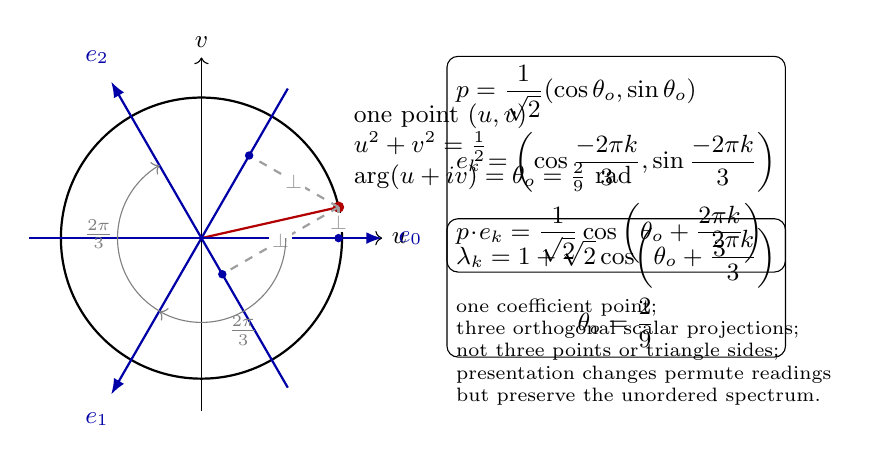
\begin{tikzpicture}[
  scale=1.02,
  every node/.style={font=\small},
  heading/.style={-{Latex[length=2mm]}, thick, blue!65!black},
  projection/.style={dashed, gray!75, thick}
]
\coordinate (O) at (0,0);
\pgfmathsetmacro{\thetaDeg}{(2/9)*180/pi}
\pgfmathsetmacro{\stepDeg}{360/3}
\def\radius{1.75}
\draw[thick] (O) circle (\radius);
\draw[->] (-2.15,0)--(2.25,0) node[right] {\(u\)};
\draw[->] (0,-2.15)--(0,2.25) node[above] {\(v\)};
\coordinate (P) at ({\radius*cos(\thetaDeg)},{\radius*sin(\thetaDeg)});
\fill[red!70!black] (P) circle (2pt);
\draw[thick, red!70!black] (O)--(P);
\node[above right=1mm of P, align=left]
  {one point \((u,v)\)\\
   \(u^2+v^2=\frac12\)\\
   \(\arg(u+iv)=\theta_o=\frac29\ {\rm rad}\)};
\foreach \idx in {0,1,2}{
  \pgfmathsetmacro{\headingAngle}{-\idx*\stepDeg}
  \pgfmathsetmacro{\projectionLength}
    {\radius*cos(\thetaDeg-\headingAngle)}
  \coordinate (F\idx) at
    ({\projectionLength*cos(\headingAngle)},
     {\projectionLength*sin(\headingAngle)});
  \draw[heading]
    ({-2.15*cos(\headingAngle)},{-2.15*sin(\headingAngle)})
    --({2.25*cos(\headingAngle)},{2.25*sin(\headingAngle)})
    node[pos=1.08] {\(e_{\idx}\)};
  \draw[projection] (P)--(F\idx)
    node[midway,fill=white,inner sep=1pt,font=\scriptsize] {\(\perp\)};
  \fill[blue!65!black] (F\idx) circle (1.5pt);
}
\draw[->,gray] (1.05,0) arc[start angle=0,end angle=-120,radius=1.05];
\node[gray] at (.52,-1.15) {\(\frac{2\pi}{3}\)};
\draw[->,gray] (-.52,-.91) arc[start angle=-120,end angle=-240,radius=1.05];
\node[gray] at (-1.28,.05) {\(\frac{2\pi}{3}\)};
\node[draw,rounded corners,align=left,anchor=west] at (3.05,.92)
  {\(\displaystyle
    p=\frac1{\sqrt2}(\cos\theta_o,\sin\theta_o)\)\\[3pt]
   \(\displaystyle
    e_k=\left(\cos\frac{-2\pi k}{3},
              \sin\frac{-2\pi k}{3}\right)\)\\[3pt]
   \(\displaystyle
    p\!\cdot\!e_k
    =\frac1{\sqrt2}\cos\left(
      \theta_o+\frac{2\pi k}{3}\right)\)};
\node[draw,rounded corners,align=center,anchor=west] at (3.05,-.62)
  {\(\displaystyle
    \lambda_k=1+\sqrt2\cos\!\left(
      \theta_o+\frac{2\pi k}{3}\right)\)\\[3pt]
   \(\displaystyle\theta_o=\frac29\)};
\node[align=left,anchor=west,font=\scriptsize] at (3.05,-1.42)
  {one coefficient point;\\
   three orthogonal scalar projections;\\
   not three points or triangle sides;\\
   presentation changes permute readings\\
   but preserve the unordered spectrum.};
\end{tikzpicture}
\caption{Three \(C_3\) scalar projections of one selected coefficient point.
The point angle is calculated directly from \(\theta_o=2/9\) radians.  The
three axes are generated at \(2\pi/3\) separation, and each dashed segment is
the perpendicular from the same point to its corresponding projection axis.
These are three cyclic scalar readings, not three independent coefficient
points and not a spatial triangle.  A presentation change may permute the
ordered readings but preserves the unordered spectrum.}
\label{fig:c3-spectral-projections}
\end{figure}

\Needspace{7\baselineskip}
\section{The Exact \texorpdfstring{\(206\)}
\label{sec:13}{206}-to-\texorpdfstring{\(409\)}{409} Construction}
The intrinsic middle-to-minimum ratio is greater than \(206\) and less than \(207\). This section first proves that interval without measured input. It then uses the one-event/two-preserved-face recovery record to construct the finite count \(409\). The spectrum supplies \(206\); the recovery record supplies the two-face structure needed to combine two \(206\)-element supports. Figure \(\ref{fig:observer-betweenness}\) summarizes observer-rooted middle placement, while Figure \(\ref{fig:two-face-409}\) separately summarizes free amalgamation over the common three-root carrier.

\Needspace{5\baselineskip}
\subsection{Exact Determination of \texorpdfstring{\(206\)}{206}}
With the local Taylor variable

\begin{equation*}
\begin{adjustbox}{max width=\linewidth,center}
$\displaystyle
x:=\theta_o=\frac29,
$
\end{adjustbox}
\end{equation*}
one has

\begin{equation*}
\begin{adjustbox}{max width=\linewidth,center}
$\displaystyle
\lambda_{\min}
=
1-\frac{\cos x}{\sqrt2}
-\frac{\sqrt6}{2}\sin x,
$
\end{adjustbox}
\end{equation*}
\begin{equation*}
\begin{adjustbox}{max width=\linewidth,center}
$\displaystyle
\lambda_{\mathrm{mid}}
=
1-\frac{\cos x}{\sqrt2}
+\frac{\sqrt6}{2}\sin x.
$
\end{adjustbox}
\end{equation*}
% LAYOUT_ONLY_GUARD:PELL_FIRST_CERTIFICATE_CHAIN
\Needspace{18\baselineskip}
Because \(0<x<1\), the alternating Taylor theorem gives finite rational upper and lower bounds for \(\sin x\) through degree nine and for \(\cos x\) through degree eight. The exact Pell certificates

\begin{equation*}
\begin{adjustbox}{max width=\linewidth,center}
$\displaystyle
2(470832)^2-(665857)^2=-1,
\qquad
2(1136689)^2-(1607521)^2=1
$
\end{adjustbox}
\end{equation*}
% LAYOUT_ONLY_GUARD:PELL_BOUND_GIVE
\Needspace{7\baselineskip}
give

\begin{equation*}
\begin{adjustbox}{max width=\linewidth,center}
$\displaystyle
\frac{470832}{665857}
<
\frac1{\sqrt2}
<
\frac{1136689}{1607521},
$
\end{adjustbox}
\end{equation*}
% LAYOUT_ONLY_GUARD:PELL_SECOND_CERTIFICATE_CHAIN
\Needspace{16\baselineskip}
while

\begin{equation*}
\begin{adjustbox}{max width=\linewidth,center}
$\displaystyle
4(1046629)^2-6(854569)^2=-2,
\qquad
4(4656965)^2-6(3802396)^2=4
$
\end{adjustbox}
\end{equation*}
% LAYOUT_ONLY_GUARD:PELL_BOUND_GIVE
\Needspace{7\baselineskip}
give

\begin{equation*}
\begin{adjustbox}{max width=\linewidth,center}
$\displaystyle
\frac{1046629}{854569}
<
\frac{\sqrt6}{2}
<
\frac{4656965}{3802396}.
$
\end{adjustbox}
\end{equation*}
Sign-aware rational interval propagation yields

\begin{equation*}
\begin{adjustbox}{max width=\linewidth,center}
$\displaystyle
206\lambda_{\min}^2
<
\lambda_{\mathrm{mid}}^2
<
207\lambda_{\min}^2.
$
\end{adjustbox}
\end{equation*}
Since \(\lambda_{\min}>0\),

\begin{equation}
\label{eq:206-interval}
\begin{adjustbox}{max width=\linewidth,center}
$\displaystyle
\boxed{
206
<
R_{\mathrm{mid}/\min}^{\mathrm{int}}
=
\left(
\frac{\lambda_{\mathrm{mid}}}{\lambda_{\min}}
\right)^2
<
207.
}
$
\end{adjustbox}
\end{equation}
Consequently,

\begin{equation*}
\begin{adjustbox}{max width=\linewidth,center}
$\displaystyle
\boxed{
n_{\mathrm{mid}}
:=
\left\lfloor
R_{\mathrm{mid}/\min}^{\mathrm{int}}
\right\rfloor
=206,
}
$
\end{adjustbox}
\end{equation*}
and \(\rho_{\mathrm{mid}}=R_{\mathrm{mid}/\min}^{\mathrm{int}}-206\in(0,1)\). No decimal and no measured muon value participates in this result.

\Needspace{5\baselineskip}
\subsection{Two Supports Attached to the Preserved Faces}
The carried record supplies one event, its two preserved faces, and

\begin{equation*}
\begin{adjustbox}{max width=\linewidth,center}
$\displaystyle
(n_{\mathrm{post}},n_{\mathrm{route}})=(2,1).
$
\end{adjustbox}
\end{equation*}
% LAYOUT_ONLY_GUARD:ROOT_CARRIER_SEQUENCE
\Needspace{18\baselineskip}
Attach two \(206\)-element supports to the two preserved faces. Let

\begin{equation*}
\begin{adjustbox}{max width=\linewidth,center}
$\displaystyle
C=C_{\mathrm{root}}=\{r_0,r_1,r_2\},
\qquad
|C|=3,
$
\end{adjustbox}
\end{equation*}
% LAYOUT_ONLY_GUARD:ROOT_SUPPORT_DEFINITION
\Needspace{13\baselineskip}
be the common \(C_3\) root carrier. Let \(U_{\mathrm{dir}}\) and \(U_{\mathrm{route}}\) be disjoint \(203\)-element sets, each disjoint from \(C\), and define

\begin{equation*}
\begin{adjustbox}{max width=\linewidth,center}
$\displaystyle
\Gamma_{\mathrm{dir}}
=
C\sqcup U_{\mathrm{dir}},
\qquad
\Gamma_{\mathrm{route}}
=
C\sqcup U_{\mathrm{route}}.
$
\end{adjustbox}
\end{equation*}
Then

\begin{equation*}
\begin{adjustbox}{max width=\linewidth,center}
$\displaystyle
|\Gamma_{\mathrm{dir}}|
=
|\Gamma_{\mathrm{route}}|
=
3+203
=206,
\qquad
\Gamma_{\mathrm{dir}}\cap\Gamma_{\mathrm{route}}=C.
$
\end{adjustbox}
\end{equation*}
In plain terms, two 206-element supports are attached to the two preserved faces. They are not \(206\) physical events.

The subtraction term has independent provenance: \(3=|C|\) is the cardinality of the common \(C_3\) root carrier. It is not obtained from \(n_{\mathrm{post}}+n_{\mathrm{route}}=2+1\), despite the numerical equality. The face counts distinguish two aspects of one event; they do not supply the overlap removed in the amalgamation.

\Needspace{5\baselineskip}
\subsection{The Free Pushout}
Form the free pushout

\begin{equation*}
\begin{adjustbox}{max width=\linewidth,center}
$\displaystyle
\Gamma_{\mathrm{scr}}
=
\Gamma_{\mathrm{dir}}
\amalg_C
\Gamma_{\mathrm{route}},
$
\end{adjustbox}
\end{equation*}
which identifies precisely the two copies of each element of \(C\) and introduces no other relation. At least three reductions are required because duplicated common roots would double-count the same-event carrier. At most three are permitted because freeness introduces no relation among the \(406\) non-root elements and non-erasure forbids deleting them. Therefore

\begin{equation}
\label{eq:pushout-409}
\begin{adjustbox}{max width=\linewidth,center}
$\displaystyle
\boxed{
|\Gamma_{\mathrm{scr}}|
=
206+206-|C|
=
206+206-3
=409.
}
$
\end{adjustbox}
\end{equation}
Equation \(\eqref{eq:pushout-409}\) is the complete count; the two face counts do not supply its subtraction term.

The alternative \(412\) double-counts the common roots. The alternative \(406\) requires additional identifications or erasures. Only \(409\) preserves same-event identity, freeness, and non-erasure.

\Needspace{5\baselineskip}
\subsection{The Finite-Screen Factor}
For a completed count \(N\ge3\), equal completed units and one-winding closure force the successor cycle to a regular \(N\)-gon on a unit-diameter circle, up to an overall rotation and carried orientation. Each side has length \(\sin(\pi/N)\), so

\begin{equation*}
\begin{adjustbox}{max width=\linewidth,center}
$\displaystyle
\pi_L(N)=N\sin\frac{\pi}{N},
\qquad
s_N=\frac{N\sin(\pi/N)}{\pi}.
$
\end{adjustbox}
\end{equation*}
At \(N=409\),

\begin{equation}
\label{eq:screen-factor}
\begin{adjustbox}{max width=\linewidth,center}
$\displaystyle
\boxed{
s_{409}
=
\frac{409\sin(\pi/409)}{\pi},
\qquad
0<s_{409}<1.
}
$
\end{adjustbox}
\end{equation}
The exact factor used below is Eq. \(\eqref{eq:screen-factor}\).

\Needspace{5\baselineskip}
\subsection{Observer-Rooted Middle Placement}
The middle-only action is fixed before the finite factor is applied. The lawful ancestry chain and the intrinsic rank chain are

\begin{equation*}
\begin{adjustbox}{max width=\linewidth,center}
$\displaystyle
A\prec B\prec D,
\qquad
\min\prec\operatorname{mid}\prec\max.
$
\end{adjustbox}
\end{equation*}
Here \(D\) is the endpoint label in the ancestry chain; it is not the geometric filled-share invariant denoted by the same letter in Section 4. The geometric use has type

\begin{equation*}
\begin{adjustbox}{max width=\linewidth,center}
$\displaystyle
D_{\mathrm{geom}}=\frac{\pi}{3\sqrt2},
$
\end{adjustbox}
\end{equation*}
whereas the ancestry use is the terminal label in the ordered relational chain. The completed four-cell context and the independently established active coefficient also admit the typed count composite

\begin{equation*}
\begin{adjustbox}{max width=\linewidth,center}
$\displaystyle
4m
=
4\left(\frac1{2\pi}\right)
=
\frac2\pi.
$
\end{adjustbox}
\end{equation*}
This is neither an equality with \(D_{\mathrm{geom}}\) nor a redefinition of either use of \(D\). The two readings meet only at the typed completed four-cell relational location: one describes the geometric filled share, while the other names an ancestry endpoint inside the four-cell observer construction.

The first chain has the unique interior vertex \(B\), and the second has the unique middle rank. A lawful observer readout is a bijective, betweenness-preserving map

\begin{equation*}
\begin{adjustbox}{max width=\linewidth,center}
$\displaystyle
\mathcal R:
\{A,B,D\}
\longrightarrow
\{\min,\operatorname{mid},\max\}.
$
\end{adjustbox}
\end{equation*}
It must therefore carry the unique interior source element to the unique middle target:

\begin{equation}
\label{eq:observer-middle}
\begin{adjustbox}{max width=\linewidth,center}
$\displaystyle
\boxed{
\mathcal R(B)=\operatorname{mid}.
}
$
\end{adjustbox}
\end{equation}
Equation \(\eqref{eq:observer-middle}\) fixes the unique middle placement without changing the intrinsic spectrum.

Reversal may exchange the two endpoints, but it fixes the unique middle. This is observer-rooted asymmetry in its operative form: the intrinsic unordered spectrum is unchanged, while a lawful report depends on the observer's rooted ancestry and betweenness position. The finite-screen action below is therefore selected by observer-rooted betweenness, not by a particle label or by choosing a displayed spectral sector.

The factor acts once, after quadratic-support formation, and only on the middle rank:

\begin{equation*}
\begin{adjustbox}{max width=\linewidth,center}
$\displaystyle
\boxed{
(q_{\min},q_{\mathrm{mid}},q_{\max})
\longmapsto
(q_{\min},s_{409}q_{\mathrm{mid}},q_{\max}).
}
$
\end{adjustbox}
\end{equation*}
% LAYOUT_ONLY_GUARD:STANDALONE_THUS
\Needspace{7\baselineskip}
Thus

\begin{equation*}
\begin{adjustbox}{max width=\linewidth,center}
$\displaystyle
\boxed{
R_{\mathrm{mid}/\min}^{\mathrm{scr}}
=
s_{409}R_{\mathrm{mid}/\min}^{\mathrm{int}},
\qquad
R_{\max/\min}^{\mathrm{scr}}
=
R_{\max/\min}^{\mathrm{int}}.
}
$
\end{adjustbox}
\end{equation*}
Because \(s_{409}>0\), division by it recovers the intrinsic middle ratio. The construction has produced \(206\), \(409\), and \(s_{409}\) without using a measured muon or tau value.


% ALT TEXT: Four cells are shown inside one dashed relational-system boundary. A is the origin, with arrows A to B, A to C, and B to D; C and D are co-present at the same depth, giving A greater than B greater than the tied pair C equals D. A note says that one system cell carries the separately established observer/reference role but that this theorem does not identify that cell with B. Below, the strict restriction A before B before D maps to minimum before middle before maximum, forcing R of B to equal middle. Another note records 4m equals 2 over pi and warns that ancestry D is not the geometric filled share D.
\begin{figure}[t]
\centering
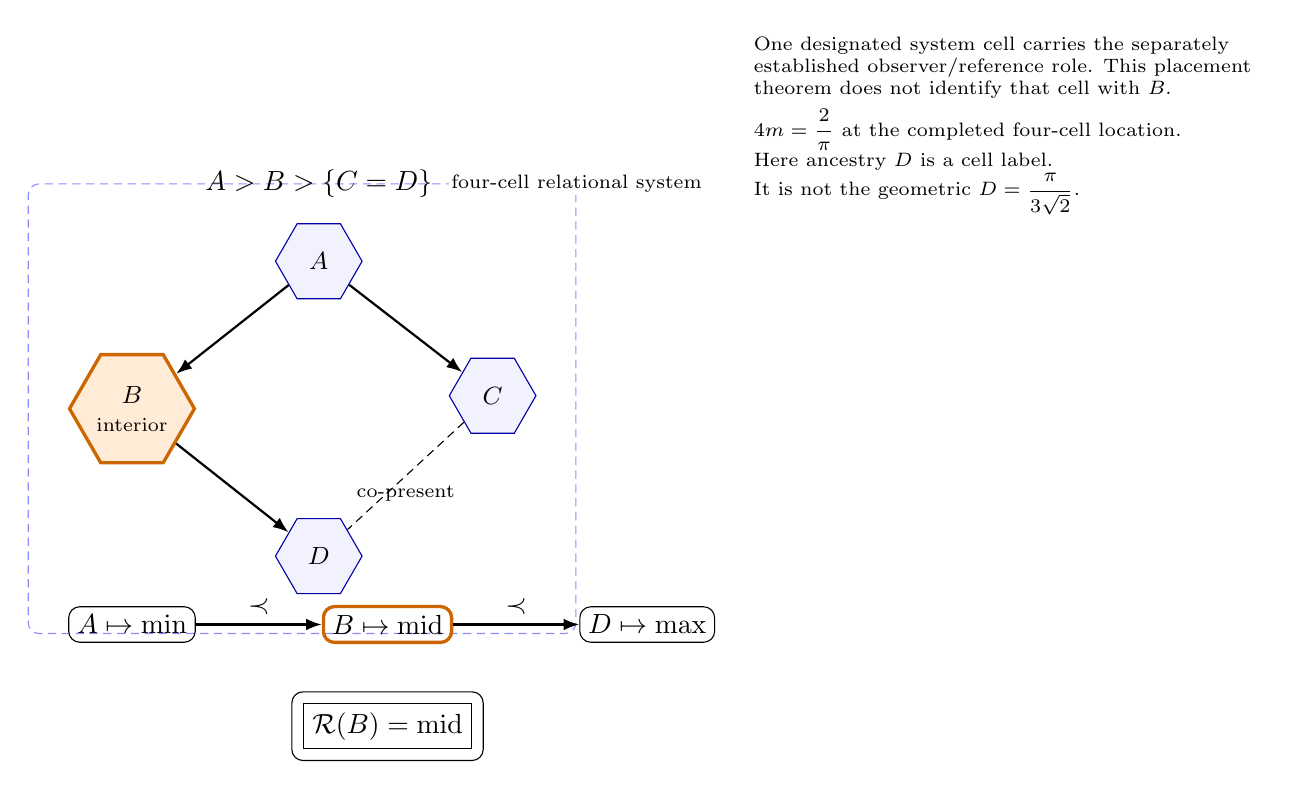
\begin{tikzpicture}[
  node distance=8mm and 16mm,
  cell/.style={regular polygon,regular polygon sides=6,draw=blue!65!black,
    fill=blue!5,minimum size=11mm,inner sep=1pt,font=\small},
  interior/.style={regular polygon,regular polygon sides=6,
    draw=orange!80!black,fill=orange!16,very thick,
    minimum size=13mm,inner sep=1pt,font=\small,align=center},
  rank/.style={draw,rounded corners,minimum width=16mm,inner sep=3pt},
  arrow/.style={-{Latex[length=2mm]},thick}
]
\node[cell] (A) {\(A\)};
\node[interior, below left=10mm and 15mm of A] (B)
  {\(B\)\\[-1pt]\scriptsize interior};
\node[cell, below right=10mm and 15mm of A] (C) {\(C\)};
\node[cell, below right=10mm and 15mm of B] (D) {\(D\)};
\draw[arrow] (A)--(B);
\draw[arrow] (A)--(C);
\draw[arrow] (B)--(D);
\draw[densely dashed] (C)--node[below,font=\scriptsize]{co-present}(D);
\node[draw=blue!45,densely dashed,rounded corners,
  fit=(A)(B)(C)(D),inner sep=5mm] (system) {};
\node[font=\scriptsize,fill=white,inner sep=1pt] at (system.north east)
  {four-cell relational system};
\node[above=2mm of A] {\(A>B>\{C=D\}\)};
\node[rank, below=18mm of B] (amin) {\(A\mapsto\min\)};
\node[rank, right=of amin,draw=orange!80!black,very thick]
  (bmid) {\(B\mapsto\operatorname{mid}\)};
\node[rank, right=of bmid] (dmax) {\(D\mapsto\max\)};
\draw[arrow] (amin)--node[above]{\(\prec\)}(bmid);
\draw[arrow] (bmid)--node[above]{\(\prec\)}(dmax);
\node[draw,rounded corners,below=6mm of bmid,inner sep=4pt]
  {\(\boxed{\mathcal R(B)=\operatorname{mid}}\)};
\node[align=left,font=\scriptsize,anchor=west] at (5.4,1.72)
  {One designated system cell carries the separately\\
   established observer/reference role.  This placement\\
   theorem does not identify that cell with \(B\).\\[3pt]
   \(4m=\dfrac2\pi\) at the completed four-cell location.\\
   Here ancestry \(D\) is a cell label.\\
   It is not the geometric \(D=\dfrac{\pi}{3\sqrt2}\).};
\end{tikzpicture}
\caption{Observer-rooted ancestry and middle placement.  The observer is the
separately established role of one cell within the relational system, not an
external eye or frame; this diagram does not assign that role to \(B\).  The
invariant lineage arrows are \(A\to B\), \(A\to C\), and \(B\to D\), with
\(C\) and \(D\) co-present.  Betweenness on the restricted chain
\(A\prec B\prec D\) forces the ancestry-interior element \(B\) to the middle
rank under the lawful observer readout.  The ancestry label \(D\) and the
geometric filled-share symbol \(D\) are distinguished by type; the displayed
four-cell composite does not identify their numerical values.}
\label{fig:observer-betweenness}
\end{figure}

% ALT TEXT: Two recoverably distinct preserved presentations of one event, Gamma sub dir and Gamma sub route, each have 206 elements and overlap in one common three-root carrier. Free amalgamation gives 206 plus 206 minus 3 equals 409. The resulting regular-screen factor is then shown acting exactly once, after quadratic-support formation, only on the observer-selected middle entry of the three-rank tuple.
\begin{figure}[t]
\centering
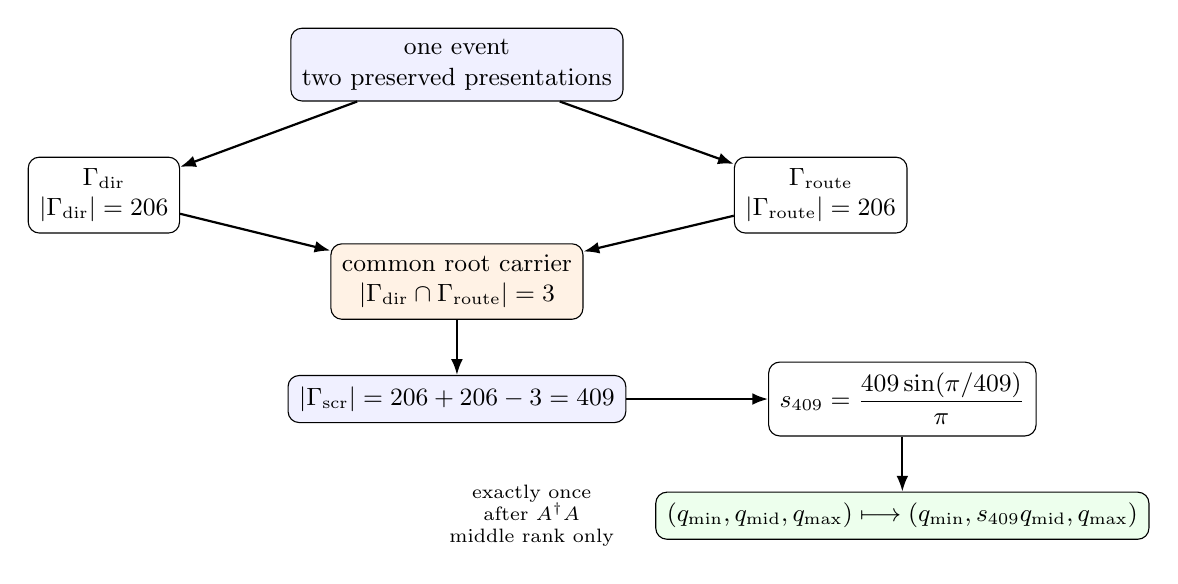
\begin{tikzpicture}[
  node distance=7mm and 14mm,
  box/.style={draw,rounded corners,align=center,inner sep=4pt,font=\small},
  arrow/.style={-{Latex[length=2mm]},thick}
]
\node[box,fill=blue!6] (event) {one event\\two preserved presentations};
\node[box,below left=of event] (dir)
  {\(\Gamma_{\rm dir}\)\\ \(|\Gamma_{\rm dir}|=206\)};
\node[box,below right=of event] (route)
  {\(\Gamma_{\rm route}\)\\ \(|\Gamma_{\rm route}|=206\)};
\node[box,below=18mm of event,fill=orange!10] (root)
  {common root carrier\\
   \(|\Gamma_{\rm dir}\cap\Gamma_{\rm route}|=3\)};
\draw[arrow] (event)--(dir);
\draw[arrow] (event)--(route);
\draw[arrow] (dir)--(root);
\draw[arrow] (route)--(root);
\node[box,below=of root,fill=blue!6] (screen)
  {\(\displaystyle|\Gamma_{\rm scr}|=206+206-3=409\)};
\draw[arrow] (root)--(screen);
\node[box,right=18mm of screen] (factor)
  {\(\displaystyle s_{409}
    =\frac{409\sin(\pi/409)}{\pi}\)};
\draw[arrow] (screen)--(factor);
\node[box,below=of factor,fill=green!7] (action)
  {\(\displaystyle
   (q_{\min},q_{\rm mid},q_{\max})
   \longmapsto
   (q_{\min},s_{409}q_{\rm mid},q_{\max})\)};
\draw[arrow] (factor)--(action);
\node[font=\scriptsize,align=center,left=4mm of action]
  {exactly once\\after \(A^\dagger A\)\\middle rank only};
\end{tikzpicture}
\caption{Two-face free amalgamation and the \(409\)-screen action.  The two
\(206\)-element sets are recoverably distinct preserved presentations of the
same event, not independent physical events.  They share one three-root
subobject.  The resulting factor acts exactly once, after quadratic-support
formation, and only on the observer-selected middle rank.}
\label{fig:two-face-409}
\end{figure}

\Needspace{7\baselineskip}
\section{Charged-Lepton Mass Ratios and the Electron Standard}
\label{sec:14}
The preceding sections produced a strictly ordered internal support triple and one finite correction on its middle member. This section attaches downstream charged-lepton reporting names and introduces one conventional scale. The mathematics fixes the ratios before the external electron record enters.

% LAYOUT_ONLY_HEADING_GUARD:DOWNSTREAM_REPORTING_ROLES
\Needspace{10\baselineskip}
\subsection{Downstream Reporting Roles}
% LAYOUT_ONLY_GUARD:REPORTING_ROLE_MAP
\Needspace{10\baselineskip}
For reporting, define the bijective role map

\begin{equation*}
\begin{adjustbox}{max width=\linewidth,center}
$\displaystyle
\min\longmapsto e,
\qquad
\mathrm{mid}\longmapsto\mu,
\qquad
\max\longmapsto\tau.
$
\end{adjustbox}
\end{equation*}
This is a downstream naming convention over already derived ranks. It does not claim that laboratory masses selected the ordering, and it does not make a displayed sector intrinsically electron, muon, or tau.

The screened support triple is

\begin{equation*}
\begin{adjustbox}{max width=\linewidth,center}
$\displaystyle
Q_{\mathrm{scr}}
=
(q_e,q_\mu,q_\tau)
=
\left(
q_{\min},
s_{409}q_{\mathrm{mid}},
q_{\max}
\right).
$
\end{adjustbox}
\end{equation*}
Its two ratios are already fixed:

\begin{equation*}
\begin{adjustbox}{max width=\linewidth,center}
$\displaystyle
\frac{q_\mu}{q_e}
=
s_{409}
\left(
\frac{\lambda_{\mathrm{mid}}}{\lambda_{\min}}
\right)^2,
\qquad
\frac{q_\tau}{q_e}
=
\left(
\frac{\lambda_{\max}}{\lambda_{\min}}
\right)^2.
$
\end{adjustbox}
\end{equation*}
No dimensional datum is needed for these results.

\Needspace{5\baselineskip}
\subsection{One External Comparison Standard}
The recorded 2022 CODATA electron mass-energy equivalent \cite{CODATA2022} is

\begin{equation*}
\begin{adjustbox}{max width=\linewidth,center}
$\displaystyle
M_e^{\mathrm{std}}c_{\mathrm{SI}}^2
=
0.51099895069(16)\ {\rm MeV}.
$
\end{adjustbox}
\end{equation*}
MeV is an energy unit used to report the mass-energy equivalent. It is not treated as a mass unit or as theory-native structure.

% LAYOUT_ONLY_GUARD:ELECTRON_STANDARD_MAP
\Needspace{10\baselineskip}
Let \(\mathcal B\) be a positive reporting map that preserves every support ratio and sends \(q_e=q_{\min}\) to the admitted electron standard:

\begin{equation*}
\begin{adjustbox}{max width=\linewidth,center}
$\displaystyle
\mathcal B(q_e)=M_e^{\mathrm{std}},
\qquad
\frac{\mathcal B(q)}{\mathcal B(q_e)}
=
\frac{q}{q_e}.
$
\end{adjustbox}
\end{equation*}
These requirements determine the map pointwise:

\begin{equation*}
\begin{adjustbox}{max width=\linewidth,center}
$\displaystyle
\boxed{
\mathcal B(q)
=
\frac{M_e^{\mathrm{std}}}{q_e}\,q
=
\frac{M_e^{\mathrm{std}}}{m\lambda_{\min}^2}\,q.
}
$
\end{adjustbox}
\end{equation*}
% LAYOUT_ONLY_GUARD:ELECTRON_SCALE_RECOVERY_SEQUENCE
\Needspace{18\baselineskip}
The one positive scale

\begin{equation*}
\begin{adjustbox}{max width=\linewidth,center}
$\displaystyle
\mathcal S_e
:=
\frac{M_e^{\mathrm{std}}}{m\lambda_{\min}^2}
$
\end{adjustbox}
\end{equation*}
% LAYOUT_ONLY_GUARD:SUPPORT_RECOVERY_LEADIN
\Needspace{8\baselineskip}
gives \(\mathcal B(q)=\mathcal S_e q\), and the internal support is recovered by

\begin{equation*}
\begin{adjustbox}{max width=\linewidth,center}
$\displaystyle
q=\frac{\mathcal B(q)}{\mathcal S_e}.
$
\end{adjustbox}
\end{equation*}
A change of reporting unit rescales the electron standard, \(\mathcal S_e\), and all three dimensional outputs together. It leaves the dimensionless ratios, rank ordering, \(206\), \(409\), and \(s_{409}\) unchanged.

\Needspace{5\baselineskip}
\subsection{Exact Relative Report}
The complete relative charged-lepton report is

\begin{equation}
\label{eq:mass-ratio-report}
\begin{adjustbox}{max width=\linewidth,center}
$\displaystyle
\boxed{
\left(
M_e,M_\mu,M_\tau
\right)_{\mathrm{report}}
=
M_e^{\mathrm{std}}
\left(
1,\;
s_{409}
\left(
\frac{\lambda_{\mathrm{mid}}}{\lambda_{\min}}
\right)^2,\;
\left(
\frac{\lambda_{\max}}{\lambda_{\min}}
\right)^2
\right).
}
$
\end{adjustbox}
\end{equation}
Equation \(\eqref{eq:mass-ratio-report}\) is the complete exact relative report.

Equivalently,

\begin{equation*}
\begin{adjustbox}{max width=\linewidth,center}
$\displaystyle
\boxed{
M_e^{\mathrm{report}}
=
M_e^{\mathrm{std}},
}
$
\end{adjustbox}
\end{equation*}
\begin{equation*}
\begin{adjustbox}{max width=\linewidth,center}
$\displaystyle
\boxed{
M_\mu^{\mathrm{out}}
=
M_e^{\mathrm{std}}
\frac{409\sin(\pi/409)}{\pi}
\left(
\frac{
1-\frac{\cos(2/9)}{\sqrt2}
+\frac{\sqrt6}{2}\sin(2/9)
}{
1-\frac{\cos(2/9)}{\sqrt2}
-\frac{\sqrt6}{2}\sin(2/9)
}
\right)^2,
}
$
\end{adjustbox}
\end{equation*}
\begin{equation*}
\begin{adjustbox}{max width=\linewidth,center}
$\displaystyle
\boxed{
M_\tau^{\mathrm{out}}
=
M_e^{\mathrm{std}}
\left(
\frac{
1+\sqrt2\cos(2/9)
}{
1-\frac{\cos(2/9)}{\sqrt2}
-\frac{\sqrt6}{2}\sin(2/9)
}
\right)^2.
}
$
\end{adjustbox}
\end{equation*}
These exact symbolic expressions are the primary result.

For numerical diagnosis,

\begin{equation*}
\begin{adjustbox}{max width=\linewidth,center}
$\displaystyle
s_{409}
\left(
\frac{\lambda_{\mathrm{mid}}}{\lambda_{\min}}
\right)^2
=
206.768282732054172011291935636779\ldots,
$
\end{adjustbox}
\end{equation*}
\begin{equation*}
\begin{adjustbox}{max width=\linewidth,center}
$\displaystyle
\left(
\frac{\lambda_{\max}}{\lambda_{\min}}
\right)^2
=
3477.472837104598532313001225522648\ldots.
$
\end{adjustbox}
\end{equation*}
% LAYOUT_ONLY_GUARD:STANDALONE_THUS
\Needspace{7\baselineskip}
Thus

\begin{equation*}
\begin{adjustbox}{max width=\linewidth,center}
$\displaystyle
\left(
M_e,M_\mu,M_\tau
\right)_{\mathrm{report}}
=
M_e^{\mathrm{std}}
\left(
1,\;
206.768282732054172011291935636779\ldots,\;
3477.472837104598532313001225522648\ldots
\right).
$
\end{adjustbox}
\end{equation*}
Using the central electron standard gives the diagnostic mass-energy equivalents

\begin{equation*}
\begin{adjustbox}{max width=\linewidth,center}
$\displaystyle
M_e c_{\mathrm{SI}}^2
=
0.51099895069(16)\ {\rm MeV},
$
\end{adjustbox}
\end{equation*}
\begin{equation*}
\begin{adjustbox}{max width=\linewidth,center}
$\displaystyle
M_\mu^{\mathrm{out}}c_{\mathrm{SI}}^2
=
105.658375512052928326006945941653\ldots\ {\rm MeV},
$
\end{adjustbox}
\end{equation*}
\begin{equation*}
\begin{adjustbox}{max width=\linewidth,center}
$\displaystyle
M_\tau^{\mathrm{out}}c_{\mathrm{SI}}^2
=
1776.984970813427147785657684886757\ldots\ {\rm MeV}.
$
\end{adjustbox}
\end{equation*}
% LAYOUT_ONLY_GUARD:PROPAGATED_UNCERTAINTIES
\Needspace{13\baselineskip}
Propagating only the parenthetical uncertainty of the admitted electron standard through the two fixed ratios gives

\begin{equation*}
\begin{adjustbox}{max width=\linewidth,center}
$\displaystyle
\boxed{
M_\mu^{\mathrm{out}}c_{\mathrm{SI}}^2
=
105.658375512(33)\ {\rm MeV}.
}
$
\end{adjustbox}
\end{equation*}
\begin{equation*}
\begin{adjustbox}{max width=\linewidth,center}
$\displaystyle
\boxed{
M_\tau^{\mathrm{out}}c_{\mathrm{SI}}^2
=
1776.98497081(56)\ {\rm MeV}.
}
$
\end{adjustbox}
\end{equation*}
These parenthetical uncertainties contain only the propagated electron-standard uncertainty. They include neither theoretical uncertainty nor finite-screen-model uncertainty. The longer values above remain computational diagnostics.

Only the electron standard is an experimental derivation input. No measured muon or tau value determines the intrinsic spectrum, rank ordering, \(206\), \(409\), \(s_{409}\), or either ratio.

\Needspace{5\baselineskip}
\subsection{Post-Exposure Muon Consistency Comparison}
Only after the complete mass-ratio derivation is fixed do we compare its middle ratio with the 2022 CODATA recommended adjusted value \cite{CODATA2022},

\begin{equation*}
\begin{adjustbox}{max width=\linewidth,center}
$\displaystyle
R_{\mu/e}^{\mathrm{CODATA}}
=
206.7682827(46).
$
\end{adjustbox}
\end{equation*}
The difference is

\begin{equation}
\label{eq:muon-post-exposure}
\begin{adjustbox}{max width=\linewidth,center}
$\displaystyle
\boxed{
R_{\mu/e}^{\mathrm{out}}
-
R_{\mu/e}^{\mathrm{CODATA}}
=
3.2054172011\ldots\times10^{-8},
}
$
\end{adjustbox}
\end{equation}
which is

\begin{equation*}
\begin{adjustbox}{max width=\linewidth,center}
$\displaystyle
\boxed{
0.0069683\ldots
}
$
\end{adjustbox}
\end{equation*}
of CODATA's quoted standard uncertainty. The quoted uncertainty is CODATA's uncertainty only; no theoretical or finite-screen-model uncertainty has been assigned.

Equation \(\eqref{eq:muon-post-exposure}\) is a downstream comparison, not a construction equation. This comparison is not a blind held-out prediction. The \(409\) construction was developed after exposure to the muon result. No muon or tau datum is an algebraic operand, and no continuous numerical parameter is fitted. The electron supplies the reporting scale, while the post-muon-exposure development of the \(409\) construction is disclosed explicitly. The comparison has no backward role in the spectrum, the integer counts, or the finite-screen factor.

The result is a relative three-entry report anchored by one admitted electron scale. It is not an absolute prediction of the electron mass. These limitations do not alter the exact derivation of the ratios.


\Needspace{7\baselineskip}
\section{Independent Koide Validation}
\label{sec:15}
The charged-lepton report is complete before this section begins. Koide's relation \cite{KOIDE1983} did not determine the spectral phase, the three amplitudes, their rank, the quadratic-support law, \(206\), \(409\), the finite-screen factor, or the electron reporting scale. It is a post-derivation validation and not an input to any preceding construction.

Here \emph{independent} means that Koide's relation was not used as a construction input. It does not mean that the final Koide quotient is algebraically independent of the derived radius and support law.

\Needspace{5\baselineskip}
\subsection{Exact Intrinsic Consequence}
Consider the already derived positive-amplitude family in the form

\begin{equation*}
\begin{adjustbox}{max width=\linewidth,center}
$\displaystyle
\lambda_k
=
1+\eta\cos\left(
\theta+\frac{2\pi k}{3}
\right),
\qquad
k\in\mathbb Z/3\mathbb Z.
$
\end{adjustbox}
\end{equation*}
The standard three-phase trigonometric sums give

\begin{equation*}
\begin{adjustbox}{max width=\linewidth,center}
$\displaystyle
\sum_k
\cos\left(
\theta+\frac{2\pi k}{3}
\right)
=0,
$
\end{adjustbox}
\end{equation*}
and

\begin{equation*}
\begin{adjustbox}{max width=\linewidth,center}
$\displaystyle
\sum_k
\cos^2\left(
\theta+\frac{2\pi k}{3}
\right)
=\frac32.
$
\end{adjustbox}
\end{equation*}
Therefore

\begin{equation*}
\begin{adjustbox}{max width=\linewidth,center}
$\displaystyle
\sum_k\lambda_k=3,
$
\end{adjustbox}
\end{equation*}
and

\begin{equation*}
\begin{adjustbox}{max width=\linewidth,center}
$\displaystyle
\sum_k\lambda_k^2
=
3+\frac32\eta^2.
$
\end{adjustbox}
\end{equation*}
The quadratic-support law gives \(q_k=m\lambda_k^2\). Within the positive-amplitude chamber, \(\sqrt{q_k}=\sqrt m\,\lambda_k\), so the common coefficient cancels from the intrinsic Koide quotient:

\begin{equation*}
\begin{adjustbox}{max width=\linewidth,center}
$\displaystyle
Q_{\mathrm{int}}
:=
\frac{\sum_k q_k}
{\left(\sum_k\sqrt{q_k}\right)^2}
=
\frac{\sum_k\lambda_k^2}
{\left(\sum_k\lambda_k\right)^2}
=
\frac{3+\frac32\eta^2}{9}.
$
\end{adjustbox}
\end{equation*}
Consequently,

\begin{equation}
\label{eq:koide-unscreened}
\begin{adjustbox}{max width=\linewidth,center}
$\displaystyle
\boxed{
Q_{\mathrm{int}}=\frac23
\iff
\eta^2=2.
}
$
\end{adjustbox}
\end{equation}
At the selected phase \(\theta_o=2/9\), all three amplitudes are positive, and the independently derived rooted radius gives \(\eta^2=2\). Hence

\begin{equation*}
\begin{adjustbox}{max width=\linewidth,center}
$\displaystyle
\boxed{
Q_{\mathrm{int}}=\frac23
}
$
\end{adjustbox}
\end{equation*}
exactly before finite-screen rendering. This exact composite is phase-independent within the positive-amplitude chamber. It does not independently validate the selection \(\theta_o=2/9\), the amplitude hierarchy, \(206\), or \(409\); and Koide's relation was not used to construct any of them.

Equation \(\eqref{eq:koide-unscreened}\) is an exact manuscript composite of promoted identities, not a new authority statement.

\Needspace{5\baselineskip}
\subsection{Screened Koide Quotient}
The reported spectrum applies the finite-screen factor only to the middle quadratic support. Its scale-free quotient is therefore

\begin{equation}
\label{eq:koide-screened}
\begin{adjustbox}{max width=\linewidth,center}
$\displaystyle
\boxed{
Q_{\mathrm{scr}}
=
\frac{
\lambda_{\min}^2
+s_{409}\lambda_{\mathrm{mid}}^2
+\lambda_{\max}^2
}{
\left(
\lambda_{\min}
+\sqrt{s_{409}}\lambda_{\mathrm{mid}}
+\lambda_{\max}
\right)^2
}.
}
$
\end{adjustbox}
\end{equation}
Equation \(\eqref{eq:koide-screened}\) is evaluated only after the mass-ratio report has closed.

The electron comparison scale and the common coefficient \(m\) cancel. Controlled evaluation of this exact expression gives

\begin{equation*}
\begin{adjustbox}{max width=\linewidth,center}
$\displaystyle
Q_{\mathrm{scr}}
=
0.666667566724259522274262656024415\ldots,
$
\end{adjustbox}
\end{equation*}
and

\begin{equation*}
\begin{adjustbox}{max width=\linewidth,center}
$\displaystyle
Q_{\mathrm{scr}}-\frac23
=
9.00057592855607595989357748742\ldots
\times10^{-7}.
$
\end{adjustbox}
\end{equation*}
Equivalently,

\begin{equation*}
\begin{adjustbox}{max width=\linewidth,center}
$\displaystyle
\frac{Q_{\mathrm{scr}}-2/3}{2/3}
=
1.35008638928341139398403662311\ldots
\times10^{-6}.
$
\end{adjustbox}
\end{equation*}
The full algebraic departure from \(2/3\) in the reported spectrum is induced by the middle-rank finite-screen rendering. The derived report is therefore Koide-consistent at approximately the \(1.35\)-ppm level, but the screened quotient is not an exact identity.

This validation would fail if Koide's relation were used to select \(2/9\), adjust \(s_{409}\), choose \(206\) or \(409\), alter the rank assignment, or fit either mass ratio. It would also fail if the screened agreement were reported as exact equality.


\Needspace{7\baselineskip}
\section*{Conclusion}
\addcontentsline{toc}{section}{Conclusion}
This paper began from relational distinguishability and followed the consequences of that admission through positive count, persistence, conserving closure, and the derived FCC/rhombic-dodecahedral presentation. The bookkeeping matrices used along the way organize independently established quantities; their rectangular arrangement does not generate scientific authority, and no matrix algebra is used to obtain the result.

The spectral construction begins from the rooted one-cell record. Its rank-two cyclic projector fixes the one-pass action aperture, whose phase generates six presentations of one \(D_3\)-orbit. Quotienting presentation choice leaves one intrinsic unordered three-amplitude spectrum. Observer-rooted asymmetry enters only at readout: the lawful report depends on rooted ancestry and betweenness, while the unordered intrinsic spectrum remains presentation invariant. The observer does not change an intrinsic mass. The counting adjoint and complete retained incidence book then force

\begin{equation*}
\begin{adjustbox}{max width=\linewidth,center}
$\displaystyle
M_{\mathrm{read}}(A)
=
\frac1{2\pi}A^\dagger A,
$
\end{adjustbox}
\end{equation*}
and the exact intrinsic minimum, middle, and maximum support ratios.

% LAYOUT_ONLY_GUARD:CONCLUSION_MIDDLE_RATIO
\Needspace{20\baselineskip}
The middle ratio satisfies

\begin{equation*}
\begin{adjustbox}{max width=\linewidth,center}
$\displaystyle
206
<
\left(
\frac{\lambda_{\mathrm{mid}}}{\lambda_{\min}}
\right)^2
<
207,
$
\end{adjustbox}
\end{equation*}
so its integer part is \(206\). The one-event/two-preserved-face recovery record then supports two \(206\)-element sets with one independently established common three-root carrier. Their free pushout forces

\begin{equation*}
\begin{adjustbox}{max width=\linewidth,center}
$\displaystyle
409=206+206-3.
$
\end{adjustbox}
\end{equation*}
% LAYOUT_ONLY_GUARD:CONCLUSION_SCREEN_FACTOR
\Needspace{7\baselineskip}
The regular-screen factor

\begin{equation*}
\begin{adjustbox}{max width=\linewidth,center}
$\displaystyle
s_{409}
=
\frac{409\sin(\pi/409)}{\pi}
$
\end{adjustbox}
\end{equation*}
acts once on the already formed middle quadratic support.

The exact relative charged-lepton report is

\begin{equation*}
\begin{adjustbox}{max width=\linewidth,center}
$\displaystyle
\boxed{
\left(
M_e,M_\mu,M_\tau
\right)_{\mathrm{report}}
=
M_e^{\mathrm{std}}
\left(
1,\;
s_{409}
\left(
\frac{\lambda_{\mathrm{mid}}}{\lambda_{\min}}
\right)^2,\;
\left(
\frac{\lambda_{\max}}{\lambda_{\min}}
\right)^2
\right).
}
$
\end{adjustbox}
\end{equation*}
The electron record supplies the one conventional scale. It does not replace the internal coefficient, and no measured muon or tau value enters the derivation. The principal result is therefore the two exact dimensionless ratios together with their unique one-scale reporting conversion.

Before finite-screen rendering, the positive intrinsic amplitude family and quadratic-support law give the exact composite \(Q_{\mathrm{int}}=2/3\), because the independently derived radius has \(\eta^2=2\). This consequence does not select the phase or hierarchy. Only after the mass report is complete is the screened Koide functional evaluated. Its full departure from \(2/3\) is induced by the middle-rank finite-screen rendering and is approximately \(1.35\) parts per million. Koide is independent in the logical sense that it is not a derivational input; the final quotient is not claimed to be algebraically independent of the derived radius and support law.

The scope remains controlled. The result is not an absolute derivation of the electron mass, not a blind held-out prediction, not a derivation of SI units, and not a general completion of particle physics. The \(409\) construction was developed after exposure to the muon result, although no muon or tau datum is an algebraic operand and no continuous numerical parameter is fitted. It is a closure-first derivation of a charged-lepton mass-ratio structure from a count-based relational construction, with every empirical input, presentation choice, recovery record, and validation step kept in its proper logical order.


\Needspace{7\baselineskip}
\section*{Declarations}
\addcontentsline{toc}{section}{Declarations}
\textbf{Funding}

This research received no external funding.

\textbf{Competing interests}

The author declares no competing interests.

\textbf{Data availability}

No new experimental datasets were generated or analyzed in this work.


\bibliographystyle{unsrtnat}
\bibliography{references}
\end{document}
